%%%%%%%%%%%%%%%%%%%%%%%%%%%%%%%%%%%%%%%%%%%%%%%%%%%%%%%%%%%%%%%%%
%
% Project     : Bachelorarbeit
% Title       : Machbarkeitsanalyse für eine ressourcenorientierte Schnittstelle zur Verarbeitung grundlegender Probleme der Informatik
% File        : doc.tex Rev. 01
% Date        : 01.03.2015
% Author      : Raffael Santschi
%
%%%%%%%%%%%%%%%%%%%%%%%%%%%%%%%%%%%%%%%%%%%%%%%%%%%%%%%%%%%%%%%%%

%%%%%%%%%%%%%%%%%%%%%%%%%%%%%%%%%%%%%%%%%%%%%%%%%%%%%%%%%%%%%%%%%
%
% Project     : Bachelorarbeit
% Title       : Machbarkeitsanalyse für eine ressourcenorientierte Schnittstelle zur Verarbeitung grundlegender Probleme der Informatik
% File        : header.tex Rev. 01
% Date        : 01.03.2015
% Author      : Raffael Santschi
%
%%%%%%%%%%%%%%%%%%%%%%%%%%%%%%%%%%%%%%%%%%%%%%%%%%%%%%%%%%%%%%%%%

\documentclass[10pt,ngerman,pointlessnumbers]{scrreprt}

%***********************************************************************
% include some libs
%***********************************************************************
\usepackage[utf8]{inputenc}
\usepackage{listings}
\usepackage{color}
\usepackage{fancyhdr}
\usepackage{rotating}
\usepackage{mathptmx}
%\usepackage{helvet}
%\usepackage[scaled]{uarial}
%\renewcommand*\familydefault{\sfdefault} %% Only if the base font of the document is to be sans serif
\usepackage[T1]{fontenc}
\usepackage{ngerman}
\usepackage{textcomp}
\usepackage[squaren]{SIunits}
\usepackage{graphicx}
\usepackage{subfigure}
\usepackage{url}
\usepackage{geometry}
\usepackage[absolute]{textpos}
\usepackage{makeidx}
\usepackage{colortbl}
\usepackage{pdflscape}
\usepackage{pdfpages}
\usepackage{tabularx}
\usepackage{lmodern}
\usepackage{longtable}
\usepackage{array}
\usepackage{float}
\usepackage{scrhack}
\usepackage[plainpages=false]{hyperref}
\usepackage{wallpaper} %\ThisTileWallPaper{}
\usepackage[super,square]{natbib} %für BibTeX Literaturverzeichnis
\usepackage{amsmath}
\usepackage[section]{placeins}
\usepackage{booktabs}
\usepackage{todonotes}
\usepackage{slashbox}



%***********************************************************************
% various styles
%***********************************************************************	

%create index
\makeindex

%define pagestyle
\pagestyle{fancy}

%use sans-serif font 
%\renewcommand{\familydefault}{\sfdefault}

%define page margin
\geometry{a4paper, top=30mm, left=30mm, right=30mm, bottom=30mm,headsep=10mm,footskip=10mm}

%textpos parameter
%\setlength{\TPHorizModule}{30mm}
%\setlength{\TPVertModule}{\TPHorizModule}
%\textblockorigin{10mm}{10mm} % start everything near the top-left corner

%increase size of subusubseciont that is not equal to paragraph
\setkomafont{subsubsection}{\large}

%horizontal lines for titlepage 
\newcommand{\HRule}{\rule{\linewidth}{0.5mm}}

%reference to source items inlc source number
\newcommand{\srcref}[1]{\nameref{src:#1} \cite{#1}}

%own commands
\newcommand{\selfmade}[1]{(eigene Darstellung#1)}
\newcommand{\resultAssignment}[1]{#1}
\newcommand{\myTitle}[0]{Machbarkeitsanalyse für eine ressourcenorientierte Schnittstelle zur Verarbeitung grundlegender Probleme der Informatik}
\newcommand{\releaseDate}[0]{21. Januar 2015 }


%header / footer 
\renewcommand{\headrulewidth}{0.3pt}
\renewcommand{\footrulewidth}{0.3pt}
\setlength{\headheight}{35pt} 

\fancyhead[LO,RE]{} %clear headings for contents 
\fancyhead[RO,LE]{\nouppercase{\rightmark}} %right odd pages and left even pages
%\fancyhead[C]{\bfseries \myTitle~\\[0.2cm]} %right odd pages and left even pages
\fancyhead[LO,RE]{\MakeUppercase{\leftmark} ~\\[0.2cm]} %left odd pages and right even pages
\fancyfoot[LE,RO]{\thepage} %page numbering
\fancyfoot[C]{} %clear centered page numbering 

%define some colors
\definecolor{darkgreen}{RGB}{31, 135, 68}
\definecolor{gray}{rgb}{0.85,0.85,0.85}
\definecolor{darkgray}{rgb}{0.4,0.4,0.4}
%listing colors
\definecolor{lgray}{RGB}{250,250,250}
\definecolor{lgreen}{RGB}{63,127,95}
\definecolor{lred}{RGB}{127,0,85}
\definecolor{lblue}{RGB}{42,0,255}

% footnote layout optimization
\deffootnote[1.25em]{1.25em}{1.25em}{\textsuperscript{\normalfont\thefootnotemark\,}}

%***********************************************************************
% listing
%***********************************************************************

\lstset{		
		basicstyle=\small\ttfamily,
		frame=single,
		numbers=left,	
		numberstyle=\tiny,
		%firstnumber=auto,
		numberblanklines=true,
		captionpos=b,
		extendedchars=true,
		float=ht,
		showtabs=false,
		tabsize=2,
		showspaces=false,
		showstringspaces=false,
		breaklines=true,
		%prebreak=\Righttorque,
		backgroundcolor=\color{lgray},
		keywordstyle=\color{lred}\bfseries, 
		commentstyle=\color{lgreen}\ttfamily,
%		morekeywords={printstr, printhexln},
		stringstyle=\color{lblue},
		xleftmargin=0.5cm,
		xrightmargin=0.5cm
}

% Trennmuster
\hyphenation{Qualitäts-an-for-der-ung}
\hyphenation{Eintritts-wahr-schein-lichkeit}

\lstloadlanguages{Java}

%\lstdefinelanguage{xc}{
%     keywords={printstr, printhexln, attributes, class, classend, do, empty, endif, endwhile, fail, function, functionend, if, implements, in, inherit, inout, not, of, operations, out, return, set, then, types, while, use},
%     keywordstyle=\color{lred}\bfseries,
%     ndkeywords={},
%     ndkeywordstyle=\color{yellow}\bfseries,
%     identifierstyle=\color{black},
%     sensitive=false,
%     comment=[l]{//},
%     commentstyle=\color{lgreen}\ttfamily,
%     string=[l]{"},
%     stringstyle=\color{lblue}\ttfamily
%  }

\colorlet{punct}{red!60!black}
\definecolor{background}{HTML}{EEEEEE}
\definecolor{delim}{RGB}{20,105,176}
\colorlet{numb}{magenta!60!black}

\lstdefinelanguage{json}{
    basicstyle=\normalfont\ttfamily,
    numbers=left,
    stepnumber=1,
    numbersep=8pt,
    showstringspaces=false,
    breaklines=true,
    literate=
     *{0}{{{\color{numb}0}}}{1}
      {1}{{{\color{numb}1}}}{1}
      {2}{{{\color{numb}2}}}{1}
      {3}{{{\color{numb}3}}}{1}
      {4}{{{\color{numb}4}}}{1}
      {5}{{{\color{numb}5}}}{1}
      {6}{{{\color{numb}6}}}{1}
      {7}{{{\color{numb}7}}}{1}
      {8}{{{\color{numb}8}}}{1}
      {9}{{{\color{numb}9}}}{1}
      {:}{{{\color{punct}{:}}}}{1}
      {,}{{{\color{punct}{,}}}}{1}
      {\{}{{{\color{delim}{\{}}}}{1}
      {\}}{{{\color{delim}{\}}}}}{1}
      {[}{{{\color{delim}{[}}}}{1}
      {]}{{{\color{delim}{]}}}}{1}
}

\def\signed #1{{\leavevmode\unskip\nobreak\hfil\penalty50\hskip2em
    \hbox{}\nobreak\hfil(#1)%
    \parfillskip=0pt \finalhyphendemerits=0 \endgraf}}

\newsavebox\mybox
\newenvironment{myQuote}[1]
{\savebox\mybox{#1}\begin{quote}}
{\signed{\usebox\mybox}\end{quote}}



\begin{document}
%\bibliographystyle{plainnat}
%\bibliographystyle{alphadin}
\bibliographystyle{alphadin}


\title{Bachelorarbeit}
\author{Raffael Santschi}


%%%%%%%%%%%%%%%%%%%%%%%%%%%%%%%%%%%%%%%%%%%%%%%%%%%%%%%%%%%%%%%%%
%
% Project     : Bachelorarbeit
% Title       : Machbarkeitsanalyse für eine ressourcenorientierte Schnittstelle zur Verarbeitung grundlegender Probleme der Informatik
% File        : titlepage.tex Rev. 01
% Date        : 01.03.2015
% Author      : Raffael Santschi
%
%%%%%%%%%%%%%%%%%%%%%%%%%%%%%%%%%%%%%%%%%%%%%%%%%%%%%%%%%%%%%%%%%

\begin{titlepage}

% Logo
\ThisTileWallPaper{\paperwidth}{\paperheight}{images/logos/SoE.pdf} % {images/logos/*.pdf}
% Wählen Sie aus folenden pdf Files: ICP, IDP, IEFE, IMES, IMPE, IMS, INE, InES, InIT, KSR, SoE, ZAMP, ZAV, ZIL, ZPP, ZSN

\begin{minipage}[b]{0.117\textwidth}
\hskip 0.05cm
\end{minipage}
\begin{minipage}[b]{0.91\textwidth}
\begin{tiny}.\end{tiny}\vskip 2.8cm
	{\huge
	
	% Projekt Name
	\textbf{\underline{Bachelorarbeit Informatik}}\\
	
	% Projekt Titel
	
	Machbarkeitsanalyse für eine ressourcenorientierte Schnittstelle zur Verarbeitung grundlegender Probleme der Informatik
	\vskip 0.5cm}
	
	\begin{minipage}[b]{0.27\textwidth}
	\hrule\vskip 0.5cm
		\textbf{Autor}\\
		\\
		\\
		\\
	\end{minipage}
	\begin{minipage}[b]{0.03\textwidth}
	\hskip 0.5cm
	\end{minipage}
	\begin{minipage}[b]{0.7\textwidth}
	\hrule\vskip 0.5cm
		Raffael Santschi\\
		santsraf@students.zhaw.ch\\
		Student im 8. Semester\\
		\\
	\end{minipage}
	
	\begin{minipage}[b]{0.27\textwidth}
	\hrule\vskip 0.5cm
		\textbf{Hauptbetreuung}\\
		\\
		\\
	\end{minipage}
	\begin{minipage}[b]{0.03\textwidth}
	\hskip 0.5cm
	\end{minipage}
	\begin{minipage}[b]{0.7\textwidth}
	\hrule\vskip 0.5cm
		Munen Alain M. Lafon\\
		lafo@zhaw.ch\\
		\\
	\end{minipage}

	\begin{minipage}[b]{0.27\textwidth}
	\hrule\vskip 0.5cm
		\textbf{Experte}\\
		\\
		\\
	\end{minipage}
	\begin{minipage}[b]{0.03\textwidth}
	\hskip 0.5cm
	\end{minipage}
	\begin{minipage}[b]{0.7\textwidth}
	\hrule\vskip 0.5cm
		Silvan Spross\\
		silvan.spross@gmail.com\\
		\\
	\end{minipage}
	
	\begin{minipage}[b]{0.27\textwidth}
	\hrule\vskip 0.5cm
		\textbf{Abgabedatum}
	\end{minipage}
	\begin{minipage}[b]{0.03\textwidth}
	\hskip 0.5cm
	\end{minipage}
	\begin{minipage}[b]{0.7\textwidth}
	\hrule\vskip 0.5cm
		23.07.2015
	\end{minipage}

\end{minipage}
\vskip 0.5cm


\end{titlepage}

\setcounter{page}{1}
%\include{content/Kontakt}
%%%%%%%%%%%%%%%%%%%%%%%%%%%%%%%%%%%%%%%%%%%%%%%%%%%%%%%%%%%%%%%%%
%
% Project     : Bachelorarbeit
% Title       : Machbarkeitsanalyse für eine ressourcenorientierte Schnittstelle zur Verarbeitung grundlegender Probleme der Informatik
% File        : abstract.tex Rev. 01
% Date        : 01.03.2015
% Author      : Raffael Santschi
%
%%%%%%%%%%%%%%%%%%%%%%%%%%%%%%%%%%%%%%%%%%%%%%%%%%%%%%%%%%%%%%%%%

\thispagestyle{empty}


\newpage
\thispagestyle{empty}
\chapter*{Abstract}\label{abstract}
Bei einigen Problemen der Informatik werden Approximierungsalgorithmen verwenden, um eine Lösung in nützlicher Frist zu erhalten. Ziel dieser Arbeit ist eine Machbarkeitanalyse für eine 
generische Schnittstelle zur Lösung solcher Probleme. Die Schnittstelle sollte keinerlei Kenntnisse der theoretischen Informatik oder der jeweiligen Probleme voraussetzen. Dazu wurden fünf 
Probleme mit hoher Laufzeitkomplexität ausgewählt, welche nicht nur von wissenschaftlich Interesse sind. Die Problemfelder wurden auf ihre Ein- und Ausgabeparameter analysiert und die 
dazugehörigen Algorithmen betrachtet. Im späteren Verlauf der Arbeit wurde ein sechstes Problem dazugenommen, welches eine leichte Abwandlung eines bereits ausgewählten Problems ist. 
Damit konnte geprüft werden, ob sich die Implementierung der beiden Probleme generischer umsetzen lässt als bei den anderen Problemen.\\

Beim Erstellen des Konzepts wurden die Gemeinsamkeiten des Berechnungsablaufs betrachtet. Um mehr Freiheiten bei der Implementierung zu haben und eine grosse Benutzerfreundlichkeit zu 
garantieren, wurde die Nutzer- und Algorithmus-Domäne voneinander entkoppelt. Dies bot die Möglichkeit, jeweils eine andere Domänensprache zu verwenden. Zwischen den beiden Domänen 
kamen pre- und post-Aktionen zum Einsatz, welche die Datenaufbereitung für den Algorithmus beziehungsweise den Nutzer durchführten.\\

Vor der Umsetzung wurde eine Nutzwertanalyse zur Auswahl eines geeigneten Datenbanksystems durchgeführt. Nach einer Vorselektierung standen eine relationale, eine objektorientierte und 
eine dokumentorientierte Datenbank zur Auswahl. Beim Vergleich wies das dokumentorientierte Datenbanksystem mit seiner Flexibilität einen grossen Vorteil auf. Diese Flexibilität ermöglichte eine 
schnelle und unkomplizierte Implementierung und bietet dies auch für kommende Erweiterung.\\

Als Prototyp wurde ein REST API implementiert, welches die Funktionalität zur Berechnung der sechs vorher definierten Probleme bereitstellt. Hinter einem dieser Probleme wurde ein 
Algorithmus implementiert, womit der ganze Prozess getestet werden konnte. Bei den anderen Problemen wurde anhand der Recherche Ein- und Ausgabeschemata der Algorithmen definiert.\\

Das Konzept für die Schnittstelle konnte für alle sechs Probleme angewandt und der Ablauf konnte generisch gehalten werden. Das Auswahlverfahren der Probleme hat sich bewährt, die Probleme 
zeigen unterschiedliche Ausprägungen in ihrer Parametern und Lösungsweise. Einige Probleme können mit dem gleichen generischen Algorithmus gelöst werden. Zwei der Probleme, welche 
beide aus dem Bereich "`Netzwerk Design"' stammen, benötigen sehr unterschiedliche Herangehensweisen. Die Schnittstelle bietet genug Flexibilität, um ganz unterschiedliche Probleme zu behandeln und 
verschiedene Algorithmen anzusteuern. Die Machbarkeitsstudie ist als erfolgreich zu betrachten.


\includepdf{images/Erklaerung_BA.pdf} % Entsprechendes auskommentieren
% \newpage

%Inhaltsverzeichnis
\tableofcontents
\newpage



%\textbf{}
%\setcounter{page}{1}
%\pagenumbering{arabic}

%\include{content/howtoLaTeX} % Für das Schlussdokument auskommentieren

%%%%%%%%%%%%%%%%%%%%%%%%%%%%%%%%%%%%%%%%%%%%%%%%%%%%%%%%%%%%%%%%%
%
% Project     : Bachelorarbeit
% Title       : Machbarkeitsanalyse für eine ressourcenorientierte Schnittstelle zur Verarbeitung grundlegender Probleme der Informatik
% File        : uebersicht.tex Rev. 01
% Date        : 01.03.2015
% Author      : Raffael Santschi
%
%%%%%%%%%%%%%%%%%%%%%%%%%%%%%%%%%%%%%%%%%%%%%%%%%%%%%%%%%%%%%%%%%

\chapter{Problemabgrenzung}\label{chap.projektuebersicht}
Die Übersicht dient dem Zweck einen generellen Überblick über das Dokument zu verschaffen. Sie beinhaltet die Ausganglage, das Ziel dieser Arbeit, die Aufgabenstellung, die erwarteten 
Resultate und die Nicht-Ziele. Zusätzlich wird der Aufbau dieses Dokumentes erklärt.

\section{Ausgangslage}\label{ausganglage}
Bei einigen Problemen der Informatik kann deterministisch die exakte Lösung nicht in Polynomialzeit berechnet werden. Um in sinnvoller Zeit eine brauchbare Lösung zu erhalten, müssen diese 
Probleme im Allgemeinen mit Hilfe von Approximierungsalgorithmen angegangen werden. Zu dieser Kategorie gehören zum Beispiel das Problem des Handlungsreisenden oder das Rucksack 
Problem. Praktische Anwendung finden solche Probleme beispielsweise in der Logistik, bei der Routenplanung und beim Verladen von Fracht.

Die bekannten Approximierungsalgorithmen haben verschiedene Ausprägungen und auch unterschiedliche Eingabeparameter. Es gibt keine Schnittstelle für die Benutzung von diesen 
Algorithmen, welche keine detaillierte Kenntnis der darunterliegenden Probleme und Algorithmen erfordert. Eine Schnittstelle mit dieser Eigenschaft kann die Handhabung solcher Probleme 
enorm erleichtern.

\section{Ziele der Arbeit}\label{ziele}
In der Arbeit soll ein Konzept für eine Schnittstelle zur Lösung verschiedener grundlegender Probleme der Informatik erarbeitet werden. Diese Schnittstelle soll basierend auf den Erkenntnissen 
einer Analyse über die Gemeinsamkeiten dieser Approximierungsalgorithmen aufgebaut werden. Dadurch soll es einem Benutzer ermöglicht werden seine jeweiligen Probleme, beispielsweise die 
effizienten Verpackung von Gegenständen, ohne ein Verständnis der darunterliegenden Probleme der Informatik anzugehen.

Bei der Erarbeitung der Schnittstelle stehen eine geeignete Persistenz-Lösung und sowie Datenstrukturen für Ein- und Ausgabe im Vordergrund.

\section{Aufgabenstellung}\label{aufgabenstellung}
Folgende Punkte werden in der Bachelorarbeit behandelt:
\begin{enumerate}
\item Recherche von real auftretenden Problemen, welche ausschliesslich durch den Einsatz von Algorithmen mit hoher Laufzeitkomplexität gelöst werden können. Einarbeiten und Analyse in 
die ausgewählten Algorithmen.
\item Ist-Analyse der verwendeten Datenstrukturen für die Algorithmen.
\item Anforderungsanalyse einer Schnittstelle für die ausgewählten Algorithmen.
\item Erarbeiten eines Konzeptes für die Implementierung der Schnittstelle sowie einer zugehörigen Persistenz-Schicht.
\item Implementierung eines Prototypen für die Schnittstelle und der Persistenz-Schicht.
\item Automatisiertes Testen der Schnittstelle.
\end{enumerate}

\section{Erwartete Resultate}\label{erwartete_resultate}
Folgende Punkte werden als Resultate der Bachelorarbeit erwartet:
\begin{enumerate}
\item Übersicht der Probleme mit den dazugehörigen Algorithmen und Beschreibung der Algorithmen mit ihren Kerneigenschaften.
      \begin{enumerate}
        \item Ausführungen zum Einfluss der Parameter der jeweiligen Probleme auf die Komplexität.
      \end{enumerate}
\item Übersicht über die verwendeten Datenstrukturen als Input / Output der Probleme.
\item Anforderungskatalog an die Schnittstelle.
\item Konzept einer generellen Schnittstelle zur Lösung der komplexen Probleme und Datendiagramm des Datenspeichers.
\item Prototypische Implementation der Schnittstelle und des Datenspeichers.
\item Automatische Tests mit dem dazugehörigen Testprotokoll.
\end{enumerate}

\section{Nicht-Ziele}\label{nicht_ziele}
Folgende Punkte wurden mit dem Auftraggeber als Nicht-Ziele definiert und sind somit nicht Teil dieses Projekts:
\begin{itemize}
\item Der Sicherheitsaspekt einer Schnittstelle wird in diesem Projekt nicht behandelt.
\item Es werden keine Algorithmen implementiert.
\item Die Hochrechnung von Ausführungszeiten einzelner Probleme ist nicht Teil dieser Arbeit.
\end{itemize}

\section{Dokumentstruktur}\label{document_structure}
Dieses Dokument spiegelt die geleistete Arbeit wieder und ist in einzelne Kapitel unterteilt.
\begin{itemize}
\item Projektplanung: Schritte für die Erstellung des Projektplanes
\item Theoretische Grundlagen: Beschreibung der wichtigsten verwendeten Begriffe und Theorien, welche für das Verstehen der Arbeit notwendig sind
\item Analyse und Auswahl der Probleme: Erläuterung der Problemauswahl und Beschreibung der einzelnen Probleme
\item Anforderungsdokument: System- und Kontextabgrenzung, \glossarmark{Stakeholder}, getroffene Annahmen und der Anforderungskatalog mit Use Cases und Anforderungen
\item Konzept: Übersicht über das ganze System, Nutzwertanalyse der verschiedenen Datenbanktypen und die Konzeptbeschreibung der Schnittstelle
\item Umsetzung: Erkenntnisse aus dem ersten Durchstich, Implementierung des Prototyps und Beschreibung der Entwicklungsumgebung
\item Tests: Erläuterung der Test-Methoden und das Test Protokoll
\end{itemize}

Im Anhang sind das Glossar, in welchem die blau markierten Begriffe im Dokument erklärt werden, und alle Verzeichnisse zu finden. Falls es zu einem Begriff eine gängige Abkürzung gibt, 
wird diese beim ersten Auftauchen des Wortes in Klammern geschrieben und danach verwendet, im Glossar finden sich dann beide Einträge.
%%%%%%%%%%%%%%%%%%%%%%%%%%%%%%%%%%%%%%%%%%%%%%%%%%%%%%%%%%%%%%%%%
%
% Project     : Bachelorarbeit
% Title       : Machbarkeitsanalyse für eine ressourcenorientierte Schnittstelle zur Verarbeitung grundlegender Probleme der Informatik
% File        : projektplanung.tex Rev. 01
% Date        : 01.03.2015
% Author      : Raffael Santschi
%
%%%%%%%%%%%%%%%%%%%%%%%%%%%%%%%%%%%%%%%%%%%%%%%%%%%%%%%%%%%%%%%%%

\chapter{Projektplanung}\label{chap.projektplanung}
Dieses Kapitel handelt von der Projektplanung und den verschiedenen Arbeitspaketen für dieses Projekt.

\section{Meilensteine}\label{meilensteine}
Folgende Meilensteine wurden für dieses Projekt festgelegt:

\begin{table}[ht]
\centering
  \begin{tabular}{ l | r }
	\hline
	\rowcolor{gray}
	\textbf{Projektstart}			&	\textbf{23.01.2015}\\ \hline
	Anforderungsdokument fertig		&	28.02.2015	\\ \hline
	Wissen über Probleme aufgebaut		&	19.04.2015	\\ \hline
	Erster \gls{vertikaler_durchstich}		& 	26.04.2015	\\ \hline
	Architektur festgelegt			&	03.05.2015	\\ \hline
	Prototyp fertig				&	29.05.2015	\\ \hline
	Dokumentation fertig			&	12.06.2015	\\ \hline
	Dokumentation korrigiert			&	26.06.2015	\\ \hline
	Präsentation					&	08.07.2015 \\ \hline
  \end{tabular}
   \caption{Meilensteine}\label{table:milestones}
\end{table}

\section{Arbeitspakete}\label{arbeitspakete}
Das Projekt beinhaltet sieben Arbeitspakete:
\begin{itemize}
\item Planung
\item Analyse und Auswahl der Probleme
\item Requirement Engineering
\item Konzept
\item Umsetzung Prototyp
\item Testing
\item Dokumentation
\end{itemize}

\subsection{Planung}\label{planung}
In der Planungsphase wird geschaut, was in dem Projekt erreicht werden muss und wie diese Tätigkeiten auf die vorhandene Zeit aufgeteilt werden. Es wird auch das erste Mal mit dem 
Stakeholder geredet und erste Abmachungen getroffen.

\subsection{Analyse und Auswahl der Probleme}\label{analyse_auswahl_probleme}
Ein sehr wichtiges Paket ist die Analyse und die Auswahl der Probleme. Es ist wichtig, dass die Probleme möglichst vielfälltig gewählt werden und sie gut analysiert werden, damit das Konzept 
mit den erhobenen Daten sauber geplant werden kann.

\subsection{Requirement Engineering}\label{rqe}
Bei der Erstellung eines neuen Systems ist es immer wichtig, dass die Grundanforderungen bekannt sind. Um die Anforderungen zu erfassen, wird der Stakeholder befragt, was seine Wünsche 
sind. Oft werden bei der Anforderungsanalyse einige Anforderungen nicht aufgelistet, sondern einfach vorausgesetzt, sogennante \glspl{basisfaktor}, diese Anforderungen müssen dann vom 
Engineer erfasst werden. Der Anforderungskatalog wird nach der Vollendung nochmals mit dem Stakeholder in einem Review angeschaut. (siehe dazu auch \cite{req_eng_book})

\subsection{Konzept}\label{ref_backend}
Das Hauptziel dieser Arbeit ist ein Konzept, welches generisch ist und viele verschiedene Probleme mit wenig Aufwand verarbeiten kann. Die Architektur muss gut durchdacht werden und die 
Möglichkeiten gegeneinander abgewägt werden. Schlussendlich muss eine Konzept entstehen, welches in einem Prototyp umsetzbar ist.

\subsection{Umsetzung Prototyp}\label{eng_prototyp}
In diesem Arbeitspaket werden die Anforderungen mit dem festgelegten Konzept umgesetzt. Die Schnittstelle wird entworfen, die ersten Tests werden durchgeführt und Unstimmigkeiten in den 
Anforderungen werden mit dem Stakeholder geklärt.

\subsection{Testing}\label{testing}
Das Projekt benötigt automatische Tests, welche erstellt und überprüft werden müssen. Die Tests sollten einen Grossteil des Projekts abdecken und bei einer Anpassung oder Erweiterung des 
Codes Sicherheit bieten.

\subsection{Dokumentation}\label{dokumentation}
Die Dokumentation wird das ganze Projekt hindurch aktuell gehalten. Für das Erfassen dieses Dokuments wird \LaTeX\ und das \LaTeX-Template der ZHAW \cite{zhaw_latex_template} mit ein 
paar kleinen Anpassungen verwendet.

\section{Zeitplan}\label{zeitplan}
Der Zeitplan gibt eine grobe Übersicht, wann an dem Projekt gearbeitet werden kann und wann die verschiedenen Tätigkeiten fertig sein sollten. Die Angaben sind nur Richtwerte, da neben dem 
Projekt noch berufliche Verpflichtungen und andere Tätigkeiten Zeit benötigen.

\subsection{Geplante Abwesenheiten}
\begin{table}[ht]
\centering
  \begin{tabular}{ l | r }
	\hline
	\rowcolor{gray}
	\textbf{Abwesenheit}					&	\textbf{Start - Ende}	\\ \hline
	Ferien								&	07.02.2015 - 15.02.2015	\\ \hline
	Seminararbeiten						&	06.04.2015 - 19.04.2015	\\ \hline
	Modulprüfungen und Vorträge Seminararbeit		&	15.06.2015 - 28.06.2015	\\ \hline
  \end{tabular}
   \caption{Geplante Abwesenheiten}\label{table:holidays}
\end{table}

\begin{landscape}
\thispagestyle{empty}
\subsection{Projektplan}\label{projektplan}
Der Zeitplan basierend auf den Arbeitspaketen und den geplanten Abwesenheiten sieht wie folgt aus:
\begin{figure}[h]
\centering
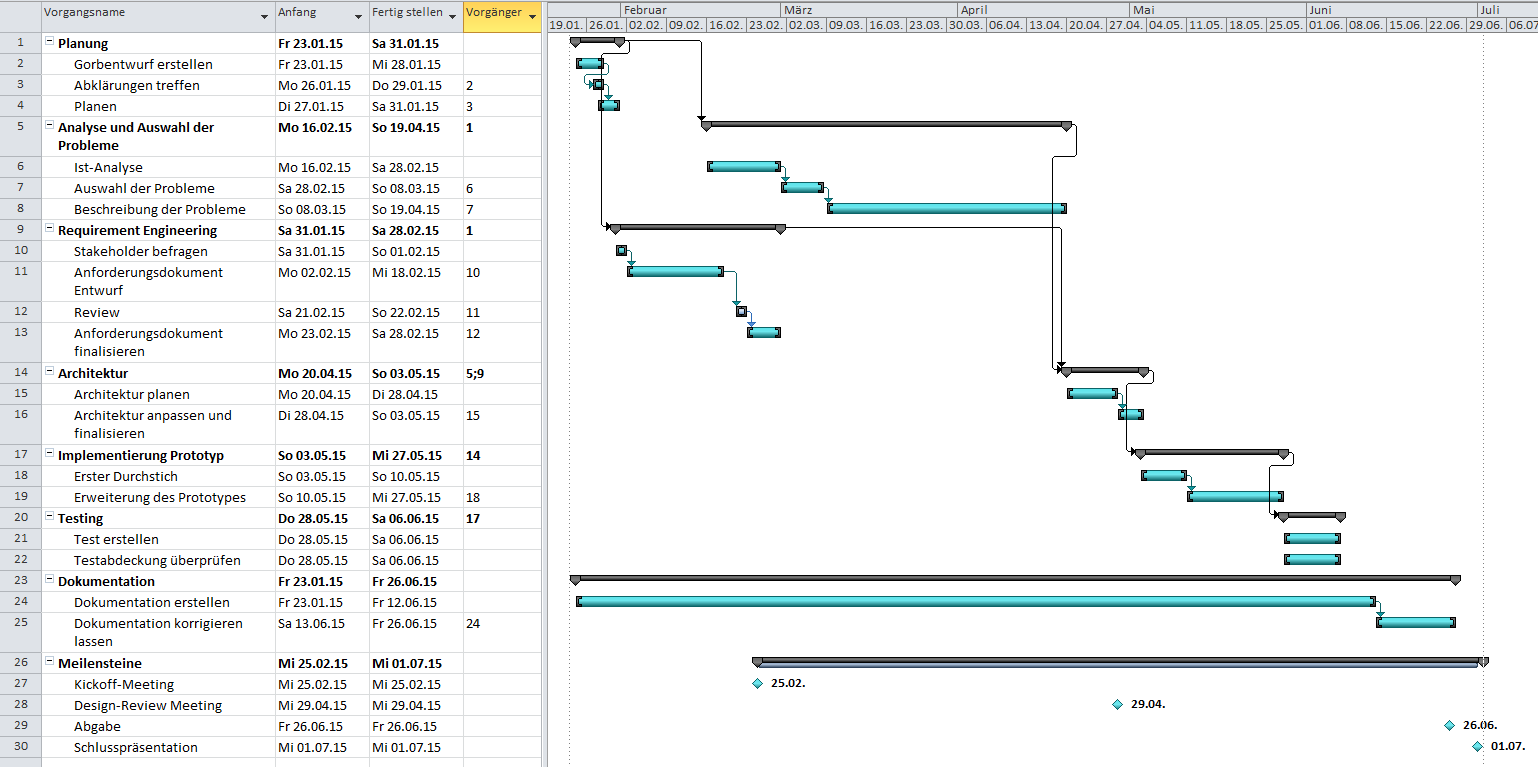
\includegraphics[scale=0.5]{images/project/projectplan.png}
\caption[Projektplan]{Projektplan \selfmade{}}
\label{fig:psp}
\end{figure}

\end{landscape}

\subsection{Zeitschätzung auf Arbeitspaketebene}
\begin{table}[ht]
\centering
  \begin{tabular}{ l | c | c }
	\hline
	\rowcolor{gray}
	\textbf{Arbeitspaket}					&	\textbf{Schätzung (h)}	& \textbf{Tatsächlich (h)}	\\ \hline
	Requirement Engineering					&	20			& 30	\\ \hline
	Reale Optimierungsprobleme suchen			&	50			& 70	\\ \hline
	Wissensaufbau Algorithmen				&	70			& 50	\\ \hline
	Konzept Planung						&	60			& 70	\\ \hline
	Prototyp Entwicklung					&	50			& 80	\\ \hline
	Tests								&	10			& 20	\\ \hline
	Dokumentation						&	120			& 100	\\ \hline \hline
	Total								&	380			& 420	\\ \hline
  \end{tabular}
   \caption{Zeitschätzung auf Arbeitspaketebene}\label{table:time_estimation}
\end{table}

\subsubsection{Erklärung der Abweichungen}
Das Requirement Engineering und Testen wurde unterschätzt, die Zeit floss jedoch vorallem in Detailarbeiten. Bei der Suche von realen Optimierungsprobleme wurde mehr Zeit beansprucht, als
ursprünglich geplant. Während der Suche konnte jedoch bereits Wissen über die Algorithmen aufgebaut werden, was dazu führte, dass in diesem Bereich weniger Zeit benötigt wurde. Als 
Evaluation des gewählten Konzept wurde ein \gls{vertikaler_durchstich} durchgeführt, was sich in der benötigten Zeit wiederspiegelt. Die Entwicklung des Prototyps war aufwändiger 
als gedacht, was daran lag, dass sechs statt fünf Probleme umgesetzt wurden. Die Dokumentation benötigte nicht so viel Zeit, jedoch ist dieser Punkt auch etwas ungenau zu 
messen, da in den anderen Paketen auch bereits Dokumentation entsteht.

%%%%%%%%%%%%%%%%%%%%%%%%%%%%%%%%%%%%%%%%%%%%%%%%%%%%%%%%%%%%%%%%%
%
% Project     : Bachelorarbeit
% Title       : Machbarkeitsanalyse für eine ressourcenorientierte Schnittstelle zur Verarbeitung grundlegender Probleme der Informatik
% File        : einleitung.tex Rev. 01
% Date        : 01.03.2015
% Author      : Raffael Santschi
%
%%%%%%%%%%%%%%%%%%%%%%%%%%%%%%%%%%%%%%%%%%%%%%%%%%%%%%%%%%%%%%%%%

\chapter{Einleitung}\label{chap.einleitung}
Die Einleitung dient dazu, wichtige Informationen zum Verständnis der Arbeit zu erläutern. Es werden die Komplexitätsklassen der Theoretischen Informatik und die verschiedenen Algorithmentypen erklärt.

\section{Komplexitätsklassen der Theoretischen Informatik}\label{cat_theo_inf}
In der Theoretischen Informatik wird zwischen verschiedenen Komplexitätsklassen unterschieden. In diesem Kapitel werden nur auf die Komplexitätsklassen NP, P, NP-schwer und NP-vollständig eingegangen, weitere Klassen wie zum Beispiel RP (Random Polynomial) oder ZPP (Zero-Error, Probabilistic, Polynomial) werden nicht erläutert, da sie nicht zum Verständnis der Arbeit notwendig sind. Die nachfolgenden Erklärungen sind aus \cite{hopcroft2011einfuehrung} und \cite{slides_p_np} abgeleitet.

\begin{figure}[h]
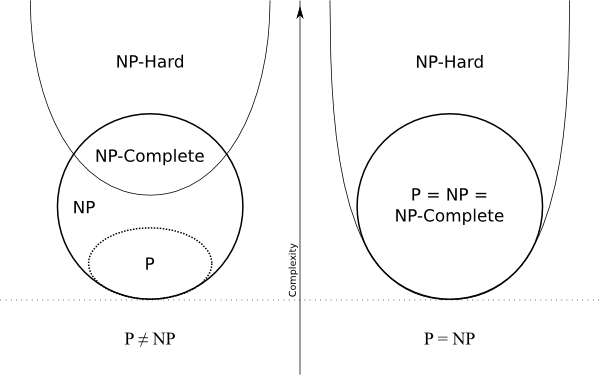
\includegraphics[scale=0.7]{images/einleitung/p_np_np-complete_np-hard.png}
\caption[Übersicht der Komplexitätsklassen ($P!=NP$ und $P=NP$)]{Übersicht der Komplexitätsklassen ($P \neq NP$ und $P=NP$) (Grafik entnommen aus \cite{pic_p_np})}
\label{fig:complexity_overview}
\end{figure}

Die Abbildung \ref{fig:complexity_overview} zeigt die Aufteilung der verschiedenen Komplexitätsklassen für die beiden Fälle $P \neq NP$ und $P=NP$. Momentan wird davon ausgegangen, dass $P \neq NP$ ist und somit die linke Aufteilung stimmt. Keine der beiden Behauptungen konnte bis jetzt bewiesen werden. Der letzte Versuche $P \neq NP$ zu beweisen wurde von Vinay Deolalikar im Jahr 2010 unternommen \cite{p_neq_np_paper}. In diesem Versuch wurden jedoch zwei Fehler entdeckt (siehe \cite{p_neq_np_paper_blog}) und somit bleibt der Beweis weiter offen.

\subsection{NP}\label{np}
Falls die Korrektheit einer Lösung zu einem Problem in polynomialer Zeit überprüft werden kann, also ein Polynomialzeit-Verifizierer vorhanden ist, liegt das Problem in NP.

\subsection{P}\label{p_complet}
Probleme, welche in polynomialer Zeit lösbar sind, gehören zu der Klasse der P-vollständigen Probleme. In polynomialer Zeit lösbar heisst, dass die Laufzeitkomplexität in einem Polynom mit der Form $n^k$, wobei n die Eingabelänge und k eine Konstante ist, dargestellt werden kann.

\subsection{NP-schwer}\label{np_hard}
Probleme, welche nicht in polynomialer Zeit lösbar sind, das heisst eine Laufzeitkomplexität höher als polynomial haben, zum Beispiel $k^n$ (exponentiell) oder $n!$ (faktoriell), gehören zu den NP-schweren Problemen. Um zu beweisen, dass das Problem NP-schwer ist, wird versucht ein anderes bekanntes NP-schweres Problem auf dieses Problem zu reduzieren. Mit diesem Beweis wird gezeigt, dass das Problem mindestens so schwer wie das andere Problem ist.

\subsection{NP-vollständig}\label{np_complet}
Stephen Cook hat mit dem Beweis der NP-Vollständigkeit des SAT-Problems (siehe \cite{cook_complexity}), die Ausgangslage für den Beweise der NP-Vollständigkeit vieler weiteren Probleme bereit gestellt. Damit ein Problem als NP-vollständig gilt, müssen folgende zwei Punkte erfüllt sein:
\begin{itemize}
	\item Ein Polynomialzeit-Verifizierer für das Problem ist vorhanden.
	\item Ein anderes bekanntes NP-vollständiges Problem ist auf dieses Problem reduzierbar.
\end{itemize}

\section{Algorithmentypen}\label{algo_types}

\subsection{Backtracking Algorithmen}\label{backtracking_algos}
Beim Backtracking geht es darum, sich einer Lösung eines Problems schrittweise zu nähern. Bei jedem neuen Schritt wird geprüft, ob es noch eine gültige Lösung darstellt. Falls dies nicht der Fall ist, wird der letzte Schritt rückgängig gemacht und es wird ein anderer Weg eingeschlagen. In \cite{backtracking} wird dieses Verfahren an Hand des Damenproblems aufgezeigt.

\subsection{Greedy Algorithmen}\label{greedy_algos}
Greedy Algorithmen liefern oft eine schnelle Lösung, welche aber meist nicht optimal ist. Die Algorithmen entscheiden bei jedem Schritt, was die aktuell beste Möglichkeit ist. Da sie nicht alle Möglichkeiten betrachten, finden sie oft nur ein lokales Minimum bzw. Maximum. In \autoref{fig:greedy_algo} ist in grün der Weg des Greedy Algorithmus zu sehen. Der Algorithmus entscheidet sich für die 12 auf der zweiten Ebene, da diese in dem Moment als beste Lösung gilt. Mit dem violetten Pfad könnte jedoch einen viel höheren Wert erzielen werden.

\begin{figure}[h]
\centering 
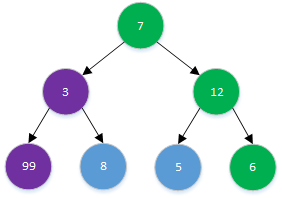
\includegraphics[scale=1]{images/einleitung/greedy_algo.png}
\caption[Suchablauf eines Greedy Algorithmus]{Suchablauf eines Greedy Algorithmus (Eigene Darstellung, Daten entnommen aus: \cite{pic_greedy_algo})}
\label{fig:greedy_algo}
\end{figure}

\subsection{Evolutionäre Algorithmen}\label{ea_algos}
Evolutionäre Algorithmen nähern sich einer optimalen Lösung an. Sie basieren auf Kombinationen (Generationen) von Objekten und einer Fitnessfunktion zur Bewertung der einzelnen Generationen. Ein Ablauf eines Evolutionären Algorithmus sieht meist wie folgt aus:
\begin{enumerate}
	\item Initialisierung: Die erste Generation wird meist zufällig erzeugt
	\item Iteration durch folgende Schritte bis die Lösung den gewünschten Wert erreicht hat:
     	\begin{enumerate}
		\item Evaluation: Mit Hilfe der Fitnessfunktion wird die erstellte Generation bewertet
         		\item Selektion: Auswahl von Objekten (Individuen) für die Rekombination
         		\item Rekombination: Erstellen einer neuen Generation durch die Kombination der ausgewählten Individuen
         		\item Mutation: Veränderung der Eigenschaften (Gene) der Nachfahren
      	\end{enumerate}
\end{enumerate}
Die Mutation und Rekombination kann positive, negative oder neutrale Eigenschaften haben. Wie in der Natur überlebt der Stärkste und somit wird die Lösung immer besser.

%%%%%%%%%%%%%%%%%%%%%%%%%%%%%%%%%%%%%%%%%%%%%%%%%%%%%%%%%%%%%%%%%
%
% Project     : Bachelorarbeit
% Title       : Machbarkeitsanalyse für eine ressourcenorientierte Schnittstelle zur Verarbeitung grundlegender Probleme der Informatik
% File        : probleme.tex Rev. 01
% Date        : 01.03.2015
% Author      : Raffael Santschi
%
%%%%%%%%%%%%%%%%%%%%%%%%%%%%%%%%%%%%%%%%%%%%%%%%%%%%%%%%%%%%%%%%%

\chapter{Analyse und Auswahl der Probleme \resultAssignment{[R1]}}\label{chap.problemauswahl}
In diesem Kapitel werden verschiedene Probleme und das dazugehörige Auswahlverfahren erläutert, welche für die Erstellung der Schnittstelle betrachtet wurden.

\section{Auswahl der Probleme}\label{cat_theo_inf}
Da es in der Welt unzählige Probleme mit hoher Laufzeitkomplexität gibt, musste ein geeignetes Verfahren herausgefunden werden, mit dem verschiedene Typen dieser Probleme für die 
Schnittstelle evaluiert werden konnten. Dafür wurde eine Kategorisierung der Probleme gesucht, auf welche sich gestützt werden konnte. 'Computers and Intractability' \cite{garey1979computers} 
von Micheal Garey und David S. Johnson  ist in der Informatik ein viel zitiertes Buch und war im Jahr 2006 laut einer Studie von CiteSeer das meist zitierteste Buch der Informatik 
\cite{citeseer_algo_buch}. In diesem Buch werden verschiedene NP-vollständige und NP-schwere Probleme vorgestellt und in Kategorien unterteilt. Diese Kategorien (siehe Auflistung unten) 
werden auch benutzt, um die zu analysierenden Problem auszuwählen.

\begin{itemize}
	\item Graphentheorie
	\item Netzwerk Design
	\item Sets und Partitionen
	\item Speicher und Wiederherstellung
	\item Sequenzierung und Planung
	\item Mathematisches Programmieren
	\item Algebra und Zahlentheorie
	\item Spiele und Puzzles
	\item Logik
	\item Automaten und Sprachtheorie
	\item Programm Optimierung
	\item Sonstiges
	\item Offene Probleme
\end{itemize}

Im Rahmen dieser Arbeit konnten nicht alle Probleme angeschaut werden, deshalb wurde geschaut, ob es Probleme gibt, welche in der Realität auftreten und nicht nur rein wissenschaftliche 
Probleme sind. Aus diesen Problemen wurden dann fünf ausgewählt, bei der Auswahl wurde auch geachtet, dass die Probleme aus unterschiedlichen Kategorien kommen, jedoch wurden auch 
zwei aus der gleichen Kategorie ausgewählt, um zu analysieren wie sich diese zwei im Gegensatz zu den anderen verhalten. Die ausgewählten Probleme werden im folgenden Abschnitt 
genauer erläutert und für die weiteren Schritte der Erstellung der Schnittstelle berücksichtigt. Durch dieses Vorgehen konnte eine hohe Diversität von Problemen sichergestellt werden, 
was bei der Erstellung der Anforderungen und Architetkur hilfreich war.

\subsection{Hierarchie der Reduktion}\label{hierarchy_reduction}
Wie bereits in der Einleitung beschrieben, muss für den Beweis der NP-Vollständigkeit ein bekanntes NP-vollständiges Problem auf das Bestehende reduziert werden können. In \autoref{fig:hierarchy_reduction} ist die Hierarchie bis zu den ausgewählten Problemen aufgezeigt.

\begin{figure}[h]
\centering 
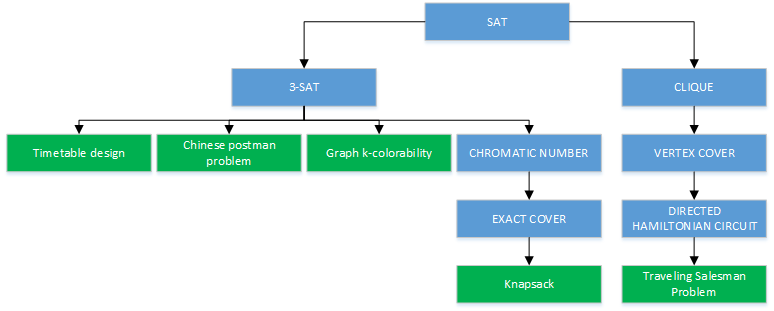
\includegraphics[scale=0.8]{images/visio/problem_hierarchy.png}
\caption[Hierarchie der Reduktion zum Beweis der NP-Vollständigkeit]{Hierarchie der Reduktion zum Beweis der NP-Vollständigkeit (Eigene Darstellung, Daten entnommen aus: \cite{garey1979computers})}
\label{fig:hierarchy_reduction}
\end{figure}

\newpage
\subsection{Graphentheorie}\label{graph_theory}

	\subsubsection{Färbung (Graphtheorie)}\label{colarability_graph_theory}
	Die Färbung in der Graphtheorie ist ein NP-vollständiges Problem. Dies wurde durch die Reduktion des 3-SAT Problemes bewiesen.

	\paragraph{Beschreibung}
	Englischer Name: Graph k-colorability

	Bei diesem Problem geht es darum die Knoten eines Graphens so zu färben, dass keine zwei benachbarten Knoten die gleiche Farbe tragen. Ein Graph heisst k-färbbar, wenn die Färbung mit k Farben korrekt durchgeführt werden kann. Dieses Problem ist für $k = 2$ in polynomieller Zeit lösbar, für $k \ge 2$ jedoch nicht mehr, dies jedoch auch nur mit gewiesen Einschränkungen (siehe \cite{garey1979computers}).

	\paragraph{Beispiel}
	Gegeben sei ein Graph mit 10 Knoten mit einer vorgegebenen Konfiguration (siehe \autoref{fig:graph_faerbung}).\\
	Gesucht ist die Färbung der Knoten, damit keine zwei benachbarten Knoten die gleiche Farbe haben, bzw. die minimale Anzahl Farben ($k$), welche verwendet werden müssen, damit die Bedingung erfüllt ist. Der Graph \ref{fig:graph_faerbung_incorrect} zeigt eine ungültige Lösung mit zwei Farben. Durch einen Algorithmus kann ermittelt werden, dass dieser Graph mindestens drei Fraben (siehe \ref{fig:graph_faerbung_correct}) benötigt, um die Bedingung zu erfüllen. Somit ist $k=3$.
\begin{figure}[ht]
\centering
\subfigure[Inkorrekte Färbung]{
  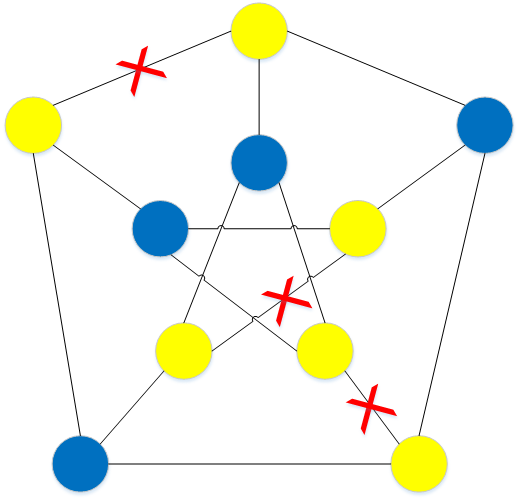
\includegraphics[scale=0.5]{images/visio/graph_faerbung_incorrect.png}
  \label{fig:graph_faerbung_incorrect}
}
\subfigure[Korrekte Färbung]{
  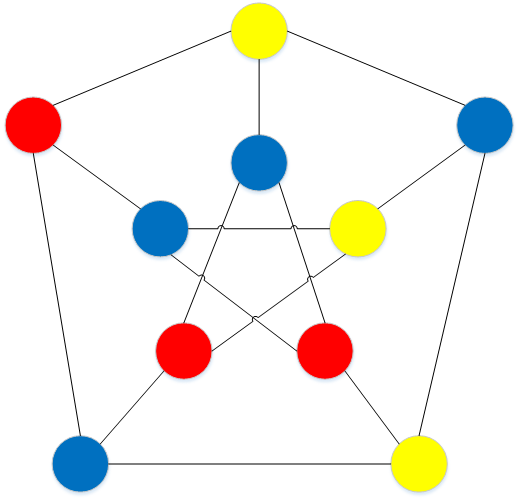
\includegraphics[scale=0.5]{images/visio/graph_faerbung_correct.png}
  \label{fig:graph_faerbung_correct}
}
\label{fig:graph_faerbung}
\caption[Kanten Färbung eines Graphen mit 10 Knoten]{Kanten Färbung eines Graphen mit 10 Knoten \selfmade{}}
\end{figure}

	\paragraph{Eingabe- und Ausgabedaten}\mbox{}\\
	Eingabedaten: Knoten mit ihren Verbindungen zu anderen Knoten\\
	Ausgabedaten: Knoten mit ihrer Färbung und $k$ (Anzahl benötigter Farben)

	\paragraph{Einfluss der Probleme auf die Komplexität}\mbox{}\\
	Bei der Knotenfärbung steigert sich die Komplexität mit Anzahl Kanten, die Knoten sind nur relevant, da sie neue Kanten aufspannen. Das die Komplexität nur von der Anzahl Kanten abhängt, zeigt auch die Formel zur Berechnung des Maximum von $k$: $k \le \frac{1}{2} + \sqrt{2m + \frac{1}{4}}$ (wobei m für die Anzahl Kanten steht) (siehe \cite{seminar_rainer_graph}). Um so grösser $k$ um so häufiger tretten Kollisionen auf und um so mehr Varianten müssen ausprobiert werden.

	\paragraph{Bekannte Algorithmen}
	(siehe \cite{seminar_algo_graph}, \cite{krumke2012graphentheoretische} und \cite{seminar_rob_graphen})
	\begin{itemize}
		\item Spalten-Generierungs-Ansatz
		\item Sequentielles Färben (Sequential Coloring)
		\item \intromark{Backtracking Algorithmus}
		\item \intromark{Greedy Algorithmus}
		\item Johnson-Algorithmus
	\end{itemize}	

	\paragraph{Bekannte reale Probleme}	
	Es gibt diverse reale Probleme, welche mit der Knotenfärbung gelöst werden können, hier sind nur einige davon aufgelistet:
	\begin{itemize}
		\item Stundenplan: Anhand der eingegebenen Daten wird ein Konfliktmatrix erstellt und diese dann in ein Färbungsproblem umgewandelt. Die Anzahl benötigten Farben sind dann die Anzahl der verschiedenen Perioden, welche es benötigt, um eine Stundenplan ohne Konflikte zu erstellen. \cite{ieee_exam_table_graph_coloring} \cite{time_table_graph_coloring}
		\item Frequenzverteilung (Mobilfunk): Im Mobilfunkt hat jede Antenne einen Frequenzbereich, im Graph werden die Antennen miteinander verwunden, bei denen die Reichweite überschneidet. Den Farben kann dann eine Frequenz zu gewiesen werden und das Resultat ist eine Konfliktfreie Mobilnetzabdeckung. \cite{seminar_rob_graphen}
		\item Färben von Landkarten: Die Länder sind die Knoten, die Kanten die Verbindung zu den Nachbarländern und die erreichnete Farbe ist die Einfärbung auf der Landkarte. \cite{seminar_rob_graphen}
	\end{itemize}

\newpage
\subsection{Netzwerk Design}\label{network_design}

	\subsubsection{Problem des Handlungsreisenden}\label{tsp}
	Das Problem des Handlungsreisenden ist ein NP-vollständiges Problem. Dies wurde durch die Reduktion des Hamiltonkreisproblemes bewiesen.

	\paragraph{Beschreibung}
	Englischer Name: Traveling Salesman Problem\\
	Beim Problem des Handlungsreisenden geht es darum mit einer optimalen Route von einem Ausgangspunkt verschiedene Wegpunkte abzufahren und wieder zum Ausgangspunkt zurück zu kehren. Es gibt verschiedene Ausprägungen des Problems, es kann zum Beispiel bestimmt werden, dass die Verbindung zwischen zwei Punkten hin und zurück gleich lang sind, was die Komplexität halbiert. Mit der Erhöhung der Anzahl Wegpunkte nimmt die Komplexität mit $O(n!)$ zu. Bei zehn Wegpunkten und ungleichen Hin- und Zurückwege sind das bereit über dreieinhalb Millionen Möglichkeiten.

	\paragraph{Beispiel} Gegeben seien vier Wegpunkte (A, B, C, D), der Startpunkt sei A.\\
	Gesucht ist die optimale Route, welche alle Wegpunkte beinhaltet und wieder bei A endet.\\
	Die Abbildung \ref{fig:tsp_example} zeigt alle möglichen Lösung mit ihren errechneten Werten. Die Route A-D-C-B-A ist mit einem Wert von 16 die beste Route. Weiter ist zu sehen, dass schon bei 4 Wegpunkten 6 Möglichkeiten vorhanden sind.
\begin{figure}[h]
\centering
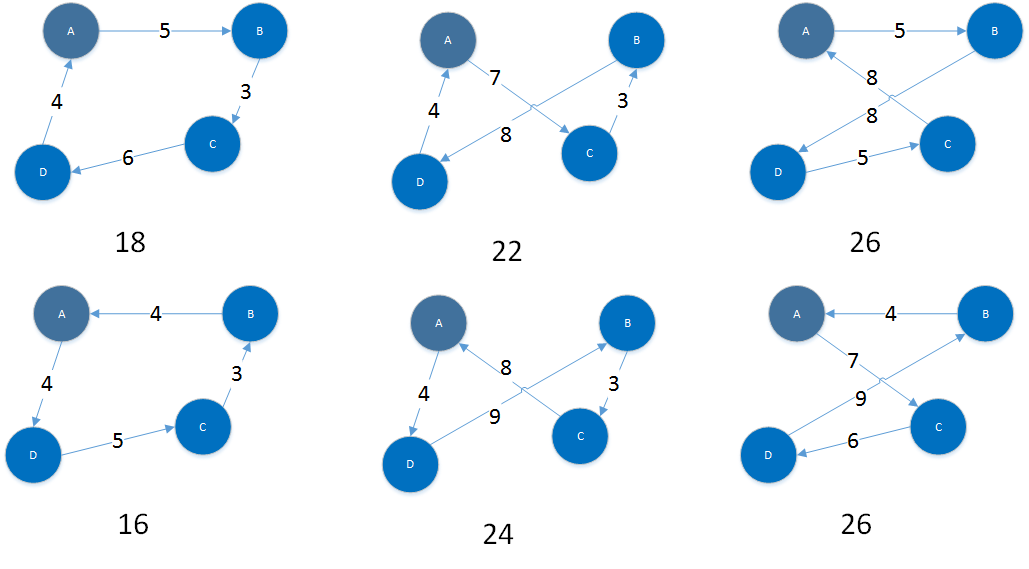
\includegraphics[scale=0.6]{images/visio/tsp.png}
\caption[Problem des Handlungsreisenden mit 4 Wegpunkten]{Problem des Handlungsreisenden mit 4 Wegpunkten \selfmade{}}
\label{fig:tsp_example}
\end{figure}

	\paragraph{Eingabe- und Ausgabedaten}\mbox{}\\
	Eingabedaten: Startpunkt und Wegpunkte, welche passiert werden müssen\\
	Ausgabedaten: Reihenfolge der Wegpunkte für eine optimale Route

	\paragraph{Einfluss der Probleme auf die Komplexität}\mbox{}\\
	Die Komplexität beim Problem des Handlungsreisenden wird durch die Anzahl Wegpunkte bestimmt.

	\paragraph{Bekannte Algorithmen}\cite{tsp_algorithmen} \cite{tsp_semesterarbeit}
	\begin{itemize}
		\item Nearest-Neighbor
		\item 2Opt
		\item Christofides
	\end{itemize}

	\subsubsection{Briefträgerproblem}\label{chinese_postman}
	Das Briefträgerproblem ist ein NP-vollständiges Problem. Dies wurde durch die Reduktion des 3-SAT Problemes bewiesen.

	\paragraph{Beschreibung}
	Englischer Name: Chinese postman problem\\
	Das Briefträgerproblem ist ähnlich wie das Problem des Handlungsreisenden, jedoch geht es darum jede Kante mindestens ein Mal abzufahren. Die Knoten stellen Kreuzungen dar, die Kanten sind Strassen. Die minimale Länge kann mit Hilfe des \glossarmark{Eulerischenkreises} relativ einfach berechnet werden. Falls der Graph die Kriterien des \glossarmark{Eulerischenkreises} nicht erfüllt, werden alle Knoten mit ungeraden Anzahl von Kanten mit einem anderen solchen Knoten über die kürzeste Route verbunden werden. Die minimal Läng ist dann alle Strecke und die Hilfsstrecken zusammen gezählt.
	\cite{pearson2004decision}

	\paragraph{Beispiel} Gegeben sei der Graph mit den Punkten A bis H und den blau eingezeichneten Verbindungen.\\
Gesucht ist eine Route mit dem kürzesten Weg, welche jede Kante mindestens ein Mal abfährt. \cite{pearson2004decision}\\
Die grün eingezeichneten Verbindungen sind Hilfslinien, um den Graph in einen \glossarmark{Eulerischenkreis} zu verwandeln. Eine mögliche Lösung mit der minimal Länge von 1000 ist die Route A-D-C-G-H-C-A-B-D-F-B-E-F-H-F-B.
\begin{figure}[h]
\centering
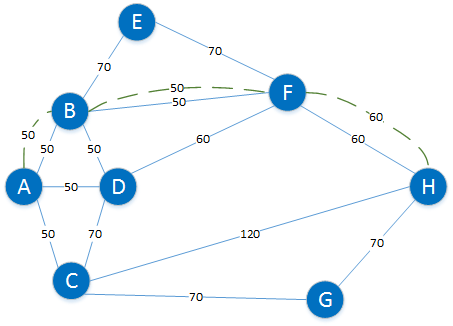
\includegraphics[scale=0.8]{images/visio/chinese_postman.png}
\caption[Beispiel für ein Briefträgerproblem]{Beispiel für ein Briefträgerproblem \selfmade{}}
\label{fig:chinese_postman_example}
\end{figure}

	\paragraph{Eingabe- und Ausgabedaten}\mbox{}\\
	Eingabedaten: Startpunkt und Knoten mit ihren Verbindungen zu anderen Knoten\\
	Ausgabedaten: Reihenfolge der Knoten für eine minimale Strecke

	\paragraph{Einfluss der Probleme auf die Komplexität}\mbox{}\\
	Wie bei der Knotenfärbung spielt hier die Anzal Kanten die Hauptrolle bei der Komplexität, die Anzahl Knoten und ob eine Graph bereits \glossarmark{eulersch} ist, spielen eine geringere Rolle.

	\paragraph{Bekannte Algorithmen}\mbox{}\\
	Briefträgeralgorithmus (Chinese postman algorithm)

\subsection{Sequenzierung und Planung}\label{sequencing_scheduling}

	\subsubsection{Stundenplan Design}\label{tsp}
	Das Erstellen eines Stundenplanes ist ein NP-vollständiges Problem. Dies wurde durch die Reduktion des 3-SAT Problemes bewiesen.

	\paragraph{Beschreibung}
	Englischer Name: Timetable design\\
	Die Erstellung von Stundenplänen ist ein sehr komplexes Problem, basierend auf Fächer, Lehrer, Klassen und Klassenzimmern wird versucht eine optimale Verteilung der Stunden zu erreichen. Die wichtigste Bedingung (hard constraints) ist, dass ein Lehrer zur selben Zeit nur jeweils 1 Fach unterrichtet und für die Klasse und das Klassenzimmer gilt dasselbe. Zusätzlich gibt es dann noch beliebig weitere Kriterien (soft constraints), wie zum Beispiel das eine Klasse nie mehr als 9 Lektionen pro Tag haben soll oder ein Lehrer nie mehr als 5 Lektionen am Stuck unterrichten sollte. Bei der Erstellung von Stundenplänen spricht man von hard constraints und soft constraints. Ein hard constraint ist im Gegensatz zu eine soft constraint unabdingbar, das heisst, es ist nicht möglich, dass ein Lehrer zwei verschiedene Fächer gleichzeitig unterrichtet, jedoch könnte er mehr als 5 Lektionen hintereinander unterrichten. \cite{Abramson92aparallel} \cite{Abramson91constructingschool} \cite{framework_timetabling} \cite{time_table_constraint_opti_ea}

	\paragraph{Beispiel} Gegeben seien die Fächer, Lehrer, Klassen und Klassenzimmer aus den Tabellen \ref{table:eg_subject}, \ref{table:eg_teacher}, \ref{table:eg_schoolclasses} und \ref{table:eg_schoolroom}.\\
Gesucht ist ein Stundenplan, bei welchem es keine Kollisionen für Lehrer, Klassen und Klassenzimmer gibt.

\begin{table}[ht]
\centering
  \begin{tabular}{ l | l }
	\hline
	\rowcolor{gray}
	\textbf{Fachname}	& \textbf{Kürzel}\\ \hline
	Mathematik		& M\\ \hline
	Deutsch		& D\\ \hline
	Englisch		& E\\ \hline
	Französisch		& F\\ \hline
	Sport			& Sp
  \end{tabular}
   \caption{Schulfächer}\label{table:eg_subject}
\end{table}

\begin{table}[ht]
\centering
  \begin{tabular}{ l | l }
	\hline
	\rowcolor{gray}
	\textbf{Lehrername} 	& \textbf{Ausbildung}\\ \hline
	Angst				& Deutsch, Mathematik, Sport\\ \hline
	Arm				& Sport\\ \hline
	Bernasconi			& Deutsch, Mathematik, Französisch\\ \hline
	Müller				& Deutsch, Mathematik, Englisch, Französisch\\ \hline
	Pfister				& Englisch, Franszösisch
  \end{tabular}
   \caption{Lehrer}\label{table:eg_teacher}
\end{table}

\begin{table}[ht]
\centering
  \begin{tabular}{ l | l }
	\hline
	\rowcolor{gray}
	\textbf{Klassenname} 	& \textbf{Benötigte Fächer}\\ \hline
	Tja13				& Deutsch, Mathematik, Sport\\ \hline
	Tja12				& Deutsch, Mathematik, Sport, Französisch\\ \hline
	Tja11				& Deutsch, Mathematik, Sport, Französisch, Englisch\\ \hline
	Tja10				& Deutsch, Mathematik, Sport, Französisch, Englisch
  \end{tabular}
   \caption{Klassen}\label{table:eg_schoolclasses}
\end{table}

\begin{table}[ht]
\centering
  \begin{tabular}{ l }
	\hline
	\rowcolor{gray}
	\textbf{Zimmername}\\ \hline
	Zimmer 101\\ \hline
	Zimmer 103\\ \hline
	Zimmer 201\\ \hline
	Turnhalle
  \end{tabular}
   \caption{Klassenzimmer}\label{table:eg_schoolroom}
\end{table}

\FloatBarrier
In der \autoref{table:timetable_1} sieht man eine mögliche Lösung zu dieser Problemstellung, dabei wurde beachtet, dass die Lehrer möglichst gleich viele Stunden unterrichten und die Schüler keine doppelten Freistunden haben. Es ist jedoch auffällig, dass das Zimmer 201 sehr schlecht ausgenützt ist, in der zweiten Variante (siehe \autoref{table:timetable_2}), wurden die Stunden der Klasse Tja11 so verschoben, dass das Zimmer 201 nicht mehr benötigt wird. Das hat jedoch zur Folge, dass die Klasse Tja11 nun eine doppelte Freistunde hat. Die Eingabedaten sind in diesem Beispiel noch sehr überschaubar, doch es gibt schon bereits enorm viele verschiedenen Möglichkeite und Ausprägungen.

\begin{table}[ht]
\centering
  \begin{tabular}{ l | l | l | l | l }
	\hline
	\rowcolor{gray}
	\textbf{Uhrzeit} 	& \textbf{Turnhalle}	& \textbf{Zimmer 101} 	& \textbf{Zimmer 103}	&  \textbf{Zimmer 201}\\ \hline
	0800-0900		& Sp / Tja13 / Arm		& D / Tja11 / Müller		& 				& \\ \hline
	0900-1000		& Sp / Tja13 / Arm		& M / Tja11 / Müller		& F / Tja12 / Pfister		& \\ \hline
	1000-1100		& Sp / Tja12 / Arm		& D / Tja10 / Bernasconi	& M / Tja13 / Angst		& F / Tja11 / Müller\\ \hline
	1100-1200		& Sp / Tja12 / Arm		& M / Tja10 / Angst		& D / Tja13 / Bernasconi	& E / Tja11 / Pfister\\ \hline \hline
	1300-1400		& Sp / Tja11 / Angst	& F / Tja10 / Bernasconi	& D / Tja12 / Müller		& \\ \hline
	1400-1500		& Sp / Tja11 / Angst	& E / Tja10 / Pfister		& M / Tja12 / Bernasconi	& \\ \hline
	1500-1600		& Sp / Tja10 / Angst	& 				& 				& \\ \hline
	1600-1700		& Sp / Tja10 / Angst	& 				& 				& \\ \hline
  \end{tabular}
   \caption{Möglicher Stundenplan - Variante 1}\label{table:timetable_1}
\end{table}

\begin{table}[ht]
\centering
  \begin{tabular}{ l | l | l | l }
	\hline
	\rowcolor{gray}
	\textbf{Uhrzeit} 	& \textbf{Turnhalle}	& \textbf{Zimmer 101} 	& \textbf{Zimmer 103}	\\ \hline
	0800-0900		& Sp / Tja13 / Arm		& D / Tja11 / Müller		& 				\\ \hline
	0900-1000		& Sp / Tja13 / Arm		& M / Tja11 / Müller		& F / Tja12 / Pfister		\\ \hline
	1000-1100		& Sp / Tja12 / Arm		& D / Tja10 / Bernasconi	& M / Tja13 / Angst		\\ \hline
	1100-1200		& Sp / Tja12 / Arm		& M / Tja10 / Angst		& D / Tja13 / Bernasconi	\\ \hline \hline
	1300-1400		& Sp / Tja11 / Angst	& F / Tja10 / Bernasconi	& D / Tja12 / Müller		\\ \hline
	1400-1500		& Sp / Tja11 / Angst	& E / Tja10 / Pfister		& M / Tja12 / Bernasconi	\\ \hline
	1500-1600		& Sp / Tja10 / Angst	& F / Tja11 / Müller		& 				\\ \hline
	1600-1700		& Sp / Tja10 / Angst	& E / Tja11 / Pfister		& 				\\ \hline
  \end{tabular}
   \caption{Möglicher Stundenplan - Variante 2}\label{table:timetable_2}
\end{table}

\FloatBarrier
	Eine sehr gut ausgearbeitete Software ist 'Units' \cite{unit_express}, sie liefert umfangreiche Funktionen zur Erstellung von Stundenplänen und hat einen sehr ausgeklügelten Optimierungsalgorithmus.

	\paragraph{Eingabe- und Ausgabedaten}\mbox{}\\
	Eingabedaten: Fächer, Lehrer, Klassen und Klassenzimmer mit verschiedenen Einschränkungen und Zusatzinformationen\\
	Ausgabedaten: Einteilung der Fächer mit den dazugehörigen Klassen, Lehrern und Zimmer auf verschiedene Tage und Uhrzeiten, welche keine Konflikte enthält

	\paragraph{Einfluss der Probleme auf die Komplexität}\mbox{}\\
	Beim Stundenplanproblem sind es nicht etwa alle 4 Liste, welche einen hohen Einfluss auf die Komplexität haben, es sind nur die Anzahl Stunden, welche verplant werden müssen. Die Anzahl Möglichkeiten berechnet sich in, abgesehen von allfälligen Einschränkungen, so: $(Anzahl Räume * Anzahl Zeitfenster * Anzahl Lehrer)^{Anzahl Veranstaltungen}$ (vergleiche \cite{scheduling_komplex}).

	\paragraph{Bekannte Algorithmen}
	(siehe \cite{framework_timetabling})
	\begin{itemize}
		\item \intromark{Backtracking Algorithmus}
		\item \intromark{Evolutionäre Algorithmen}
		\item Constraint Logic Programming
	\end{itemize}	

	\paragraph{Bekannte ähnliche Probleme}	
	Es gibt diverse andere Planungsprobleme, welche auf dem gleichen Konzept basieren, jedoch unterschiedliche Eingabedaten und Beschränkungen haben:
	\begin{itemize}
		\item Spielplan
		\item Prüfungsplan
		\item Schichtenplanung
	\end{itemize}

\newpage
\subsection{Mathematisches Programmieren}\label{mathematical_programming}

	\subsubsection{Rucksack Problem}\label{knapsack}
	Das Rucksack Problem ist ein NP-vollständiges Problem. Dies wurde durch die Reduktion des Problemes der exakten Überdeckung bewiesen.

	\paragraph{Beschreibung}
	Englischer Name: Knapsack\\
	Beim Rucksack Problem geht es um einen Container, symbolisch der Rucksack, mit einer Gewichtsschranke, desweiteren gibt es noch Objekte, welche in den Container gepackt werden können. Diese Objekte besitzen ein Gewicht und einen Profit. Das Ziel ist es den grösst möglichen Profit zu erlangen, ohne die Gewichtsschranke zu überschreiten. \cite{knapsack_desc_web}

	\paragraph{Beispiel} Gegeben sei ein Rackete mit der Gewichtsschranke 645kg und die Objekte in Tabelle \ref{table:knapsack_objects}.\\
Gesucht ist die Objektauswahl mit dem grössten Profit, welche die Gewichtsschranke nicht überschreitet.\\
In diesem Beispiel wäre die optimale Lösung 1, 2, 3 und 5. \cite{knapsack_desc_web}

\begin{table}[ht]
\centering
  \begin{tabular}{ c | r | r }
	\hline
	\rowcolor{gray}
	\textbf{Objekt-Nr.}	&	\textbf{Gewicht in kg}	&	\textbf{Profit}\\ \hline
	1			&	153			&	232\\ \hline
	2			&	54			&	73\\ \hline
	3			&	191			&	201\\ \hline
	4			&	66			&	50\\ \hline
	5			&	239			&	141\\ \hline
	6			&	137			&	79\\ \hline
	7			&	148			&	48\\ \hline
	8			&	249			&	38
  \end{tabular}
   \caption{Knapsack Objekte mit Gewicht und Profit}\label{table:knapsack_objects}
\end{table}

	\paragraph{Eingabe- und Ausgabedaten}\mbox{}\\
	Eingabedaten: Gewichtsschranke und Elemente mit Gewicht und Nutzwert\\
	Ausgabedaten: Zusammenstellung von den Elementen mit höchstem Nutzwert

	\paragraph{Einfluss der Probleme auf die Komplexität}\mbox{}\\
	Die Komplexität des Rucksack Problem hängt von der Anzahl Objekten ab, die Gewichtsschranke trägt nicht zur Komplexität bei.

	\paragraph{Bekannte Algorithmen}
	\begin{itemize}
		\item \intromark{Backtracking Algorithmus}
		\item \intromark{Greedy Algorithmus}
		\item Algorithmus von Nemhauser und Ullmann \cite{knapsack_desc_web}
	\end{itemize}	

	\paragraph{Bekannte reale Probleme}	
	Es gibt diverse reale Probleme, welche mit der dem Rucksack Problem gelöst werden können \cite{kellerer2004knapsack}, hier sind nur einige davon aufgelistet:
	\begin{itemize}
		\item Ausschneiden von verschiedenen Stücken aus einem grossen Stück Metal oder Holz: Optimale Nutzung der Fläche(n), damit am Schluss genug Einzelstücke für das Herstellen des Endprodukt vorhanden sind.
		\item Kreditvergabe: Optimale Ausnutzung des Kreditbudget mit der Vergabe von Krediten an Kunden, welche eine Kredit über eine gewisse Höhe haben möchte und eine bestimmte Risikoeinstufung haben.
	\end{itemize}


\newpage
\subsection{Logik}\label{logic}
Die hier aufgeführten Probleme sind nur zur Vollständigkeit aufgelistet und beschrieben, sie werden nicht für die weiteren Schritte der Schnittstelle verwendet. Sie sind die Grundpfeiler der NP-Vollständigkeit, durch sie konnten zahlreiche Probleme als NP-schwer oder NP-vollständig deklariert werden.

	\subsubsection{Erfüllbarkeitsproblems der \glossarmark{Aussagenlogik} (SAT)}\label{sat}
	Das Erfüllbarkeitsproblem der Aussagenlogik ist ein NP-vollständiges Problem. Dies wurde durch Stephen A. Cook in den 1970er Jahre bewiesen \cite{cook_complexity}.

	\paragraph{Beschreibung}
	Englischer Name: Satisfiability (SAT)\\
	Beim Erfüllbarkeitsproblem der \glossarmark{Aussagenlogik} geht es darum zu überprüfen, ob eine beliebige aussagenlogische Formel erfüllbar ist.	

	\paragraph{Beispiel} Gegeben sei eine aussagenlogische Formel \ref{eq:aussagenlogik}.\\
	Gesucht ist die Antwort auf die Erfüllbarkeit dieser Formel.\\
	Die \autoref{table:sat_results} zeigt, dass die Formel für die Kombinationen 3, 4 und 8 erfüllbar ist.

	\begin{equation}
   		(A \vee B) \wedge C
  		 \label{eq:aussagenlogik}
	\end{equation}

\begin{table}[ht]
\centering
  \begin{tabular}{ c | c | c | c | c | c}
	\hline
	\rowcolor{gray}
	\textbf{Kombination-Nr.}	&	\textbf{A}	&	\textbf{B} 	& 	\textbf{C} 	&	$A \vee B$	&	\textbf{Resultat}\\ \hline
	1			&	wahr	& 	falsch	& 	falsch	&	wahr		&	falsch\\ \hline
	2			&	wahr	& 	wahr	& 	falsch	&	wahr		&	falsch\\ \hline
	\textbf{3}		&	wahr	& 	falsch	& 	wahr	&	wahr		&	\textbf{wahr}\\ \hline
	\textbf{4}		&	wahr	& 	wahr	& 	wahr	&	wahr		&	\textbf{wahr}\\ \hline
	5			&	falsch	& 	falsch	& 	falsch	&	falsch		&	falsch\\ \hline
	6			&	falsch	& 	wahr	& 	falsch	&	wahr		&	falsch\\ \hline
	7			&	falsch	& 	falsch	& 	wahr	&	falsch		&	falsch\\ \hline
	\textbf{8}		&	falsch	& 	wahr	& 	wahr	&	wahr		&	\textbf{wahr}\\ \hline
  \end{tabular}
   \caption{Wahrheitstabelle zur aussagenlogischen Formel}\label{table:sat_results}
\end{table}

\newpage
	\subsubsection{3-SAT}\label{3sat}
	Das 3-SAT Problem ist ein NP-vollständiges Problem. Dies wurde durch die Reduktion des SAT Problemes bewiesen.

	\paragraph{Beschreibung}
	Englischer Name: 3-Satisfiability (3-SAT)\\
	Das 3-SAT Problem ist eine Spezialfall des SAT Problems, es dürfen maximal 3 Literale in einer Klausel enthalten sein.

	\paragraph{Beispiel} Gegeben sei eine 3-SAT Formel \ref{eq:aussagenlogik_3sat}.\\
	Gesucht ist die Antwort auf die Erfüllbarkeit dieser Formel.\\
	Die \autoref{table:3sat_results} beweisst, dass die Formel erfüllbar ist, lediglich für die Kombinationen 5, 11, 13 und 15 ist sie nicht korrekt.

	\begin{equation}
   		(A \wedge B \wedge C) \vee (B \wedge \neg C \wedge D)
  		 \label{eq:aussagenlogik_3sat}
	\end{equation}

\begin{table}[ht]
\centering
  \begin{tabular}{ c | c | c | c | c | c | c | c}
	\hline
	\rowcolor{gray}
	\textbf{Kombination-Nr.}	& \textbf{A}	& \textbf{B} 	& \textbf{C} & \textbf{D}  & $A \wedge B \wedge C$ & $B \wedge \neg C \wedge D$	& \textbf{Resultat}\\ \hline
	\textbf{1}			& wahr	& falsch	& falsch	& wahr	& wahr			 & wahr				& \textbf{wahr}\\ \hline
	\textbf{2}			& wahr	& wahr	& falsch	& wahr	& wahr			 & wahr 				& \textbf{wahr}\\ \hline
	\textbf{3}			& wahr	& falsch	& wahr	& wahr	& wahr			 & wahr				& \textbf{wahr}\\ \hline
	\textbf{4}			& wahr	& wahr	& wahr	& wahr	& wahr			 & wahr				& \textbf{wahr}\\ \hline
	5				& falsch	& falsch	& falsch	& wahr	& falsch			 & wahr				& falsch\\ \hline
	\textbf{6}			& falsch	& wahr	& falsch	& wahr	& wahr			 & wahr				& \textbf{wahr}\\ \hline
	\textbf{7}			& falsch	& falsch	& wahr	& wahr	& wahr			 & wahr 				& \textbf{wahr}\\ \hline
	\textbf{8}			& falsch	& wahr	& wahr	& wahr	& wahr			 & wahr 				& \textbf{wahr}\\ \hline
	\textbf{9}			& wahr	& falsch	& falsch	& falsch	& wahr			 & wahr				& \textbf{wahr}\\ \hline
	\textbf{10}			& wahr	& wahr	& falsch	& falsch	& wahr			 & wahr 				& \textbf{wahr}\\ \hline
	11				& wahr	& falsch	& wahr	& falsch	& wahr			 & falsch				& falsch\\ \hline
	\textbf{12}			& wahr	& wahr	& wahr	& falsch	& wahr			 & wahr				& \textbf{wahr}\\ \hline
	13				& falsch	& falsch	& falsch	& falsch	& falsch			 & wahr				& falsch\\ \hline
	\textbf{14}			& falsch	& wahr	& falsch	& falsch	& wahr			 & wahr				& \textbf{wahr}\\ \hline
	15				& falsch	& falsch	& wahr	& falsch	& wahr			 & falsch 				& falsch\\ \hline
	\textbf{16}			& falsch	& wahr	& wahr	& falsch	& wahr			 & wahr 				& \textbf{wahr}\\ \hline
  \end{tabular}
   \caption{Wahrheitstabelle zur 3-SAT Formel}\label{table:3sat_results}
\end{table}

\newpage
\subsection{Übersicht Eingabe- und Ausgabedaten \resultAssignment{[R2]}}\label{overview_input_output}
Die Eingabe- und Ausgabedaten der Probleme sind sehr unterschiedlich und weisen unterschiedliche Komplexität auf. Um einen besseren Überblick zu erhalten, wurden sie in der \autoref{table:input_output} zusammengefasst.
\begin{table}[ht]
\centering
  \begin{tabular}{ p{3.5cm} | p{6cm} | p{6cm} }
	\hline
	\rowcolor{gray}
	\textbf{Problem}				& \textbf{Eingabedaten}								& \textbf{Ausgabedaten}\\ \hline
	Färbung (Graphtheorie)			& \begin{enumerate}
								\item Knoten mit ihren Verbindungen zu anderen Knoten
							   \end{enumerate}				
							&  \begin{enumerate}
								\item Knoten mit ihrer Färbung
								\item $k$ (Anzahl benötigter Farben)
							   \end{enumerate}	\\ \hline
	Problem des Handlungsreisenden		& \begin{enumerate}
								\item Startpunkt
								\item Wegpunkte, welche passiert werden müssen
							   \end{enumerate}				
							&  \begin{enumerate}
								\item Wegpunkte in der Reihenfolge der optimalen Route
								\item Länge der Strecke
							   \end{enumerate}	\\ \hline
	Briefträgerproblem	 			& \begin{enumerate}
								\item Startpunkt
								\item Knoten mit ihren Verbindungen zu anderen Knoten
							   \end{enumerate}				
							&  \begin{enumerate}
								\item Knoten in der Reihenfolge der minimalen Strecke
								\item Länge der Strecke
							   \end{enumerate}	\\ \hline
	Stundenplan Design				& \begin{enumerate}
								\item Fächer
								\item Lehrer
								\item Klassen
								\item Klassenzimmer
								\item Stundenplan Rahmenbedingungen
							   \end{enumerate}				
							&  \begin{enumerate}
								\item  Einteilung der Fächer mit den dazugehörigen Klassen, Lehrern und Zimmer auf verschiedene Tage und Uhrzeiten, welche keine Konflikte enthält
							   \end{enumerate}	\\ \hline
	Rucksack Problem				& \begin{enumerate}
								\item Gewichtsschranke
								\item Elemente mit Gewicht und Nutzwert
							   \end{enumerate}				
							&  \begin{enumerate}
								\item Zusammenstellung von den Elementen mit höchstem Nutzwert
								\item Nutzwert
							   \end{enumerate}	\\ \hline
  \end{tabular}
   \caption{Eingabe- und Ausgabedaten der ausgewählten Probleme}\label{table:input_output}
\end{table}

\newpage
\subsection{Beispiel für den Einfluss der Parameter auf die Komplexität \resultAssignment{[R1a]}}\label{example_complexity_knapsack}
Bei den Problemen wurde der Einfluss der Parameter auf die Komplexität der Probleme erwähnt, um dies zu verdeutlichen wurde ein praktisches Beispiel anhand des Rucksack Problemes gemacht.

\subsubsection{Ausgangslage}
Das Rucksackproblem hat zwei Eingabeparameter, zum einen die Gewichtsschranke und zum anderen die Elemente. Im Beispiel wurden verschiedene Anzahl Elemente verwendet und dies mit unterschiedlichen Gewichtsschranken kombiniert. Zum Vergleich wurde die Zeit gestoppt, welche der Brute Force Algorithmus benötigt, um die optimale Lösung herauszufinden.

\subsubsection{Resultat}
Die Berechnungzeit ist ungenau und bei jedem Versuch unterschiedlich, jedoch bestätigt das Resultat die Theorie, dass die Komplexität durch die Anzahl an Elemente beeinflusst wird. Die verschiedenen Berechnungszeiten wurden in der \autoref{table:example_complexity_knapsack} festgehalten. Mit einer höheren Gewichtsschranke bleibt die Berechnungszeit in etwa gleich, bei einer Erhöung der Anzahl Elemente nimmt die Komplexität jedoch sehr schnell zu.

\begin{table}[ht]
\centering
  \begin{tabular}{ l | r | r | r | r | r }
	\hline
	\rowcolor{gray}
	\backslashbox{Gewichtsschranke:}{Anzahl an Elemente:}	& \textbf{10}	& \textbf{15} 	& \textbf{18}	& \textbf{20}	& \textbf{22}\\ \hline
	\textbf{10}							& 4ms			& 23ms		& 129ms		& 1079ms		& 7267ms 	\\ \hline
	\textbf{100}							& 1ms			& 16ms		& 149ms		& 1761ms		& 6054ms	\\ \hline
	\textbf{1000}						& 1ms			& 7ms			& 595ms		& 1038ms		& 6331ms	\\ \hline
	\textbf{10000}						& 1ms			& 7ms			& 48ms		& 583ms		& 7174ms	\\ \hline
  \end{tabular}
   \caption[Berechnungszeiten zu verschiedenen Eingabeparametern für das Rucksack Problem]{Berechnungszeiten zu verschiedenen Eingabeparametern für das Rucksack Problem \selfmade{}}
   \label{table:example_complexity_knapsack}
\end{table}

In \autoref{fig:example_complexity_knapsack} kann man die exponentielle Steigerung der Berechnungsdauer mit zu nehmenden Elementen sehr schön sehen.

\begin{figure}[h]
\centering
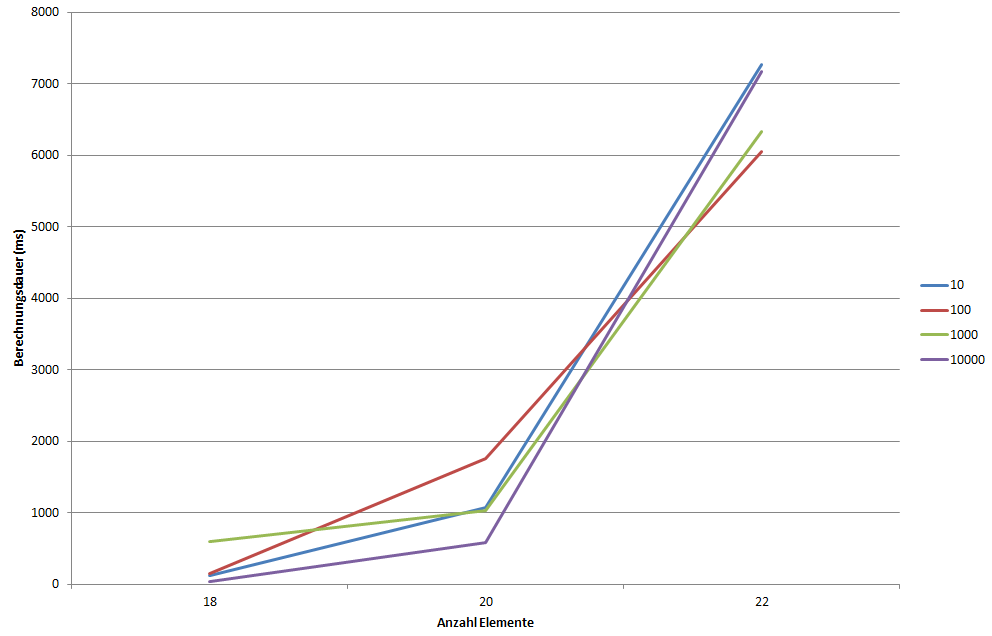
\includegraphics[scale=0.65]{images/excel/knapsack_complexity_example.png}
\caption[Berechnungszeiten für das Rucksack Problem mit verschiedenen Eingabeparametern im Vergleich]{Berechnungszeiten für das Rucksack Problem mit verschiedenen Eingabeparametern im Vergleich \selfmade{}}
\label{fig:example_complexity_knapsack}
\end{figure}

%%%%%%%%%%%%%%%%%%%%%%%%%%%%%%%%%%%%%%%%%%%%%%%%%%%%%%%%%%%%%%%%%
%
% Project     : Bachelorarbeit
% Title       : Machbarkeitsanalyse für eine ressourcenorientierte Schnittstelle zur Verarbeitung grundlegender Probleme der Informatik
% File        : anforderungsdokument.tex Rev. 01
% Date        : 01.03.2015
% Author      : Raffael Santschi
%
%%%%%%%%%%%%%%%%%%%%%%%%%%%%%%%%%%%%%%%%%%%%%%%%%%%%%%%%%%%%%%%%%

\chapter{Anforderungsdokument \resultAssignment{[R3]}}\label{chap.anforderungsdokument}

Das Anforderungsdokument legt die Basis für die Implementation. Es ist für den Verlauf des Projekts wichtig, dass zu Beginn die Anforderungen aufgestellt werden. Bei der 
Erstellung des Anforderungsdokuments werden verschiedene Betrachtungsweisen aufgezeigt und die Anforderungen an das System in verschiedenen Detailstufen angeschaut.


\section{Übersicht}\label{anf_uebersicht}

In diesem Abschnitt  wird die System- und Kontextabgrenzung dargelegt, die Systemumgebung beschrieben, die getroffenen Annahmen festgehalten und die verschiedenen \gls{stakeholder} mit 
ihren Erwartungen aufgelistet.

\subsection{System- und Kontextabgrenzung}\label{systemabgrenzung}
Der Systemkontext umfasst alle Aspekte, die für die Anforderungen des geplanten Systems relevant sind und nicht im Rahmen der Entwicklung dieses System gestaltet werden können.
\cite{req_eng_book} 

\begin{figure}[h]
\centering
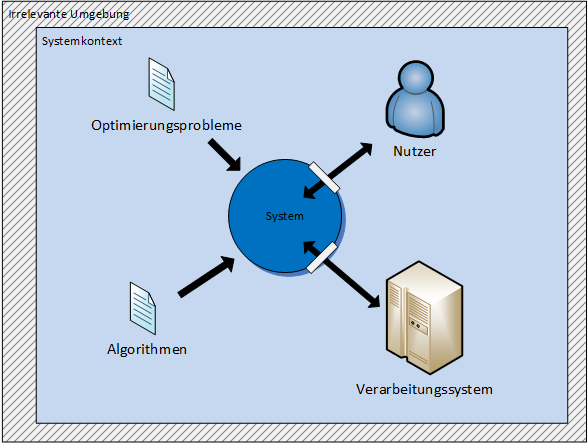
\includegraphics[scale=0.8]{images/visio/systemkontext.png}
\caption[Systemkontext]{Systemkontext \selfmade{}}
\label{fig:systemkontext}
\end{figure}

Der Systemkontext (siehe Abbildung \ref{fig:systemkontext}) zeigt, dass das System relevanten Schnittstellen zu den Nutzern und zum Verarbeitungssystem hat. Das System muss Daten 
für das Verarbeitungssystem zur Verfügung stellen und auch solche annehmen. Zudem wird das System von den Nutzern, Optimierungsproblemen und den dazugehörigen Algorithmen 
beeinflusst.

\FloatBarrier
\subsection{Systemumgebung}\label{systemumgebung}
Die Systemumgebung (siehe Abbildung \ref{fig:systemumgebung}) definiert die Ausgangslage für das Projekt. Am Anfang des Projekts war bekannt, dass Nutzer und ein Verarbeitungssystem 
Dienste des zu erstellenden Systems beziehen wird. Die genaue Ausprägung dieser Dienste werden in diesem Kapitel behandelt.

\begin{figure}[h]
\centering
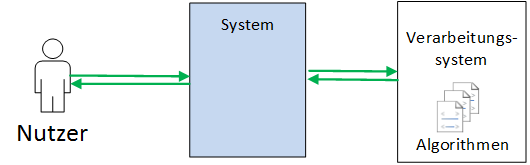
\includegraphics[scale=0.8]{images/visio/systemumgebung.png}
\caption[Systemumgebung]{Systemumgebung \selfmade{}}
\label{fig:systemumgebung}
\end{figure}

\FloatBarrier
\subsection{Annahmen}\label{annahmen}
Zwischen dem Endnutzer und dem zu erstellenden System existiert noch eine Sicherheitsschicht, welcher nicht Teil dieser Arbeit ist. Später wird dieses Projekt allenfalls um diese Sicherheitsschicht 
erweitert oder eine übergeordnete Schnittstelle erstellt, welche diese anspricht. 

Je nach Implementierung der Algorithmen ist das Ansteuern und die Aufbereitung der Daten unterschiedlich. Eine Referenzimplementierung zu jedem Problem zu finden, stellte sich als schwierig 
heraus. Deshalb wurden die Ein- und Ausgabe-Schemata der Algorithmen aus der Literaturrecherche abgeleitet.

\newpage
\subsection{Stakeholder}\label{stakeholder}
Die \gls{stakeholder}-Analyse dient dem Erfassen aller Nutzergruppen, die Einfluss auf das Projekt haben können. Zudem ermöglicht sie die Erfassung aller Gruppen, die potenziell 
Anforderungen an das Projekt stellen. In \autoref{table:stakeholder} wurden die \gls{stakeholder} dieses Projekts zusammengetragen und ihre Erwartungen, ihre 
Einstellung und ihr Einfluss gegenüber dem Projekt festgehalten. Da es sich um eine Machbarkeitsanalyse handelt, befinden sich nur der Auftraggeber und ein einzelner potenzieller Kunde in der 
Auflistung.

\begin{table}[ht]
\centering
  \begin{tabular}{ p{5cm} | p{5cm} | p{1.5cm} | p{1.5cm} }
	\hline
	\rowcolor{darkgray}
	\textbf{Name}					&	\textbf{Erwartung}	&	\textbf{Einstellung} 	&	\textbf{Einfluss}	\\ \hline
	\rowcolor{gray}
								&				&	-Positiv \mbox{-Neutral} \mbox{-Negativ} 	&	-Hoch \mbox{-Mittel} \mbox{-Niedrig} \\ \hline
	\textbf{Phil Hofmann} (Vorsteher der Geschäftsführung der 200ok GmbH)						
								&	Phil ist der Auftraggeber in diesem Projekt. Er erwartet von der Machbarkeitsanalyse Informationen für ein mögliches Projekt zur 
									Umsetzung der Gesamtidee.
												& 	Positiv		&	Hoch		\\ \hline
	\textbf{Potenzieller Kunde}
								&	Er wünscht sich eine einfache Abwicklung für seine Probleme, er möchte sich nicht mit Algorithmen und 
									theoretischer Informatik herumschlagen.
												& 	Positiv		&	Hoch		\\ \hline
  \end{tabular}
   \caption{Liste der \gls{stakeholder}}\label{table:stakeholder}
\end{table}

\newpage
\section{Anforderungen}\label{sec.anfoderungen}
Zum Erfassen der Anforderungen an das System wurden zuerst verschiedene Use Cases definiert, mit deren Hilfe anschliessend der Anforderungskatalog erstellt werden konnte.

\subsection{Use Cases}\label{use_cases}
Das Use Case Diagramm (siehe Abbildung \ref{fig:use_case}) zeigt einen Akteur, ein System und sechs Use Cases, welche für diese Arbeit relevant sind.
\begin{figure}[h]
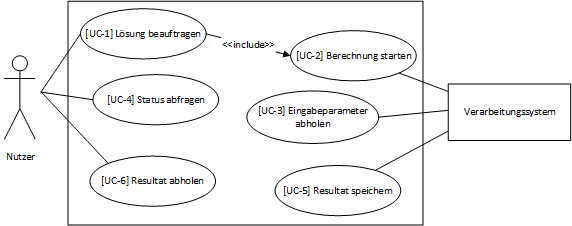
\includegraphics{images/anforderungen/use_cases.png}
\caption[Use-Case Diagramm]{Use-Case Diagramm \selfmade{}}
\label{fig:use_case}
\end{figure}

Alle Use Cases wurden anhand der folgenden Vorlage (siehe Tabelle \ref{table:use_case_template}) spezifiziert. Diese Vorlage basiert auf Angaben von \cite{req_eng_book}.

\begin{table}[ht]
\centering
  \begin{tabular}{ l | p{10cm} }
	\hline
	\rowcolor{gray}
	\textbf{Bezeichner}&	\textbf{Eindeutiger Bezeichner}\\ \hline
	\textbf{Name}		&	Eindeutiger Name\\ \hline
	\textbf{Beschreibung}	&	Komprimierte Beschreibung\\ \hline
	\textbf{Auslösendes Ereignis} &	Angabe des Ereignisses, das den Use Case auslöst.\\ \hline
	\textbf{Akteure}		&	Auflistung der Akteure, die mit dem Use Case in Beziehung stehen.\\ \hline
	\textbf{Vorbedingung}	&	Eine Liste notwendiger Voraussetzungen, die erfüllt sein müssen, bevor die Ausführung des Use Case beginnen kann.\\ \hline
	\textbf{Nachbedingung}	&	Eine Liste von Zuständen, in denen sich das System unmittelbar nach der Ausführung des Hauptszenarios befindet.\\ \hline
	\textbf{Ergebnis}		&	Beschreibung der Ausgaben, die während der Ausführung des Use Case erzeugt werden.\\ \hline
	\textbf{Hauptszenario}	&	Beschreibung des Hauptszenarios eines Use Case\\ \hline
	\textbf{Alternativszenarien}	&	Beschreibung von Alternativszenarien des Use Case oder lediglich Angabe der auslösenden Ereignisse. 
					Hier gelten oftmals andere Nachbedingungen.\\ \hline
  \end{tabular}
   \caption{Vorlage für Use Case Spezifikation}\label{table:use_case_template}
\end{table}

\begin{table}[ht]
\centering
  \begin{tabular}{ l | p{10cm} }
	\hline
	\rowcolor{gray}
	\textbf{Bezeichner}	&	\textbf{UC-1}\\ \hline
	\textbf{Name}		&	Lösung beauftragen\\ \hline
	\textbf{Beschreibung}	&	Ein Nutzer möchte eine Lösung eines Problem mit spezifischen Parametern beauftragen.\\ \hline
	\textbf{Auslösendes Ereignis} &	Nutzer möchte ein Problem lösen.\\ \hline
	\textbf{Akteure}		&	Nutzer\\ \hline
	\textbf{Vorbedingung}	&	Das System bietet zur Lösung dieses Problems eine Schnittstelle.\\ \hline
	\textbf{Nachbedingung}	&	Das System hat die nötigen Informationen für die Lösung des Problems und der Nutzer erhält eine ID, mit welcher er den Status bzw. das Resultat 
						abfragen kann.\\ \hline
	\textbf{Ergebnis}		&	Erfassung der Informationen für die Lösung des Problems\\ \hline
	\textbf{Hauptszenario}	&	\begin{enumerate}
					\item Der Nutzer ruft die Funktion für das zu lösende Problem mit den Parametern auf.
					\item Das System speichert die Parameter für die weitere Verarbeitung.
					\item Der Nutzer erhält eine ID für das Abrufen des Status bzw. des Resultats.
					\end{enumerate}
					\\ \hline
	\textbf{Alternativszenarien}	&	\begin{enumerate}
					\item[3a] Der Nutzer erhält eine Fehlermeldung, wenn das Problem nicht korrekt erfasst werden konnte.
					\end{enumerate}
					\\ \hline
  \end{tabular}
   \caption{Use Case UC-1: Lösung beauftragen}\label{table:use_case_1}
\end{table}

\begin{table}[ht]
\centering
  \begin{tabular}{ l | p{10cm} }
	\hline
	\rowcolor{gray}
	\textbf{Bezeichner}	&	\textbf{UC-2}\\ \hline
	\textbf{Name}			&	Berechnung starten\\ \hline
	\textbf{Beschreibung}	&	Das System startet die Berechnung beim Verarbeitungssystem.\\ \hline
	\textbf{Auslösendes Ereignis} &	Nutzer möchte ein Problem lösen.\\ \hline
	\textbf{Akteure}		&	Verarbeitungssystem\\ \hline
	\textbf{Vorbedingung}	&	Die Informationen für die Lösung des Problems sind erfasst.\\ \hline
	\textbf{Nachbedingung}	&	Das Verarbeitungssystem beginnt mit der Berechnung.\\ \hline
	\textbf{Ergebnis}		&	Starten der Berechnung\\ \hline
	\textbf{Hauptszenario}	&	\begin{enumerate}
					\item Das System startet die Berechnung. 
					\item Das System übergibt eine ID für das Abrufen der abgelegten Daten.
					\end{enumerate}
					\\ \hline
	\textbf{Alternativszenarien}	&	\begin{enumerate}
					\item[2a] Das System speichert die Fehlermeldung, falls das Starten der Berechnung fehlschlägt.
					\end{enumerate}
					\\ \hline
  \end{tabular}
   \caption{Use Case UC-2: Berechnung starten}\label{table:use_case_2}
\end{table}

\begin{table}[ht]
\centering
  \begin{tabular}{ l | p{10cm} }
	\hline
	\rowcolor{gray}
	\textbf{Bezeichner}	&	\textbf{UC-3}\\ \hline
	\textbf{Name}			&	Eingabe Parameter abholen\\ \hline
	\textbf{Beschreibung}	&	Das Verarbeitungssystem benötigt für die Lösung des Problems die Eingabeparameter.\\ \hline
	\textbf{Auslösendes Ereignis}&	Das Verarbeitungssystem startet eine neue Berechnung.\\ \hline
	\textbf{Akteure}		&	Verarbeitungssystem\\ \hline
	\textbf{Vorbedingung}	&	Das Verarbeitungssystem wurde angestossen, das Problem zu lösen.\\ \hline
	\textbf{Nachbedingung}	&	Das Verarbeitungssystem hat die Eingabeparameter erhalten.\\ \hline
	\textbf{Ergebnis}		&	Erhalt von Eingabeparametern\\ \hline
	\textbf{Hauptszenario}	&	\begin{enumerate}
					\item Das Verarbeitungssystem fordert die Eingabeparameter für das zu lösende Problem an.
					\item Das System leitet die Eingabeparameter weiter.
					\item Das Verarbeitungssystem erhält die Eingabeparameter.
					\end{enumerate}
					\\ \hline
	\textbf{Alternativszenarien}	&	\begin{enumerate}
					\item[2a] Das System liefert eine Fehlermeldung zurück, falls keine Eingabeparameter vorhanden sind.
					\end{enumerate}
					\\ \hline
  \end{tabular}
   \caption{Use Case UC-3: Eingabe Parameter abholen}\label{table:use_case_3}
\end{table}


\begin{table}[ht]
\centering
  \begin{tabular}{ l | p{10cm} }
	\hline
	\rowcolor{gray}
	\textbf{Bezeichner}	&	\textbf{UC-4}\\ \hline
	\textbf{Name}			&	Status abfragen\\ \hline
	\textbf{Beschreibung}	&	Der Nutzer kann den Status einer Berechnung abfragen, da die Verarbeitung einige Zeit benötigt.\\ \hline
	\textbf{Auslösendes Ereignis}&	Der Nutzer möchte den Status der Berechnung wissen.\\ \hline
	\textbf{Akteure}		&	Nutzer\\ \hline
	\textbf{Vorbedingung}	&	Der Nutzer hat bereits eine Berechnung beauftragt und kennt die ID.\\ \hline
	\textbf{Nachbedingung}	&	Der Nutzer kennt den Status der Berechnung.\\ \hline
	\textbf{Ergebnis}		&	Kenntnis des Status\\ \hline
	\textbf{Hauptszenario}	&	\begin{enumerate}
					\item Der Nutzer fragt den Status einer Berechnung ab.
					\item Das System fragt den Status ab.
					\item Das System sendet den Status zurück.
					\item Der Nutzer erhält den Status.
					\end{enumerate}
					\\ \hline
	\textbf{Alternativszenarien}	&	\begin{enumerate}
					\item[3a] Das System sendet eine Fehlermeldung zurück, falls der Status nicht ermittelt werden kann.
					\end{enumerate}
					\\ \hline
  \end{tabular}
   \caption{Use Case UC-4: Status abfragen}\label{table:use_case_4}
\end{table}

\begin{table}[ht]
\centering
  \begin{tabular}{ l | p{10cm} }
	\hline
	\rowcolor{gray}
	\textbf{Bezeichner}	&	\textbf{UC-5}\\ \hline
	\textbf{Name}			&	Resultat speichern\\ \hline
	\textbf{Beschreibung}	&	Da die Aufrufe asynchron sind, muss das Ergebnis nach der Berechnung zwischengespeichert werden.\\ \hline
	\textbf{Auslösendes Ereignis}&	Das Verarbeitungssystem möchte das Resultat speichern.\\ \hline
	\textbf{Akteure}		&	Verarbeitungssystem\\ \hline
	\textbf{Vorbedingung}	&	Das Verarbeitungssystem hat ein Resultat berechnet.\\ \hline
	\textbf{Nachbedingung}	&	Das Resultat ist gespeichert.\\ \hline
	\textbf{Ergebnis}		&	Speicherung des Resultats\\ \hline
	\textbf{Hauptszenario}	&	\begin{enumerate}
					\item Das Verarbeitungssystem schickt das Resultat der Berechnung an das System.
					\item Das System erhält das Resultat.
					\item Das System speichert das Resultat.
					\item Das System quittiert das Erhalten des Resultats.
					\item Das Verarbeitungssystem erhält die Bestätigung.
					\end{enumerate}
					\\ \hline
	\textbf{Alternativszenarien}	&	\begin{enumerate}
					\item[4a] Das System liefert eine Fehlermeldung zurück, wenn das Resultat nicht korrekt gespeichert werden konnte.
					\end{enumerate}
					\\ \hline
  \end{tabular}
   \caption{Use Case UC-5: Resultat speichern}\label{table:use_case_5}
\end{table}

\begin{table}[ht]
\centering
  \begin{tabular}{ l | p{10cm} }
	\hline
	\rowcolor{gray}
	\textbf{Bezeichner}	&	\textbf{UC-6}\\ \hline
	\textbf{Name}			&	Resultat abholen\\ \hline
	\textbf{Beschreibung}	&	Der Nutzer holt das Resultat zu einem bestimmten Zeitpunkt ab.\\ \hline
	\textbf{Auslösendes Ereignis}&	Der Nutzer möchte das Resultat der Berechnung abholen.\\ \hline
	\textbf{Akteure}		&	Nutzer\\ \hline
	\textbf{Vorbedingung}	&	Der Nutzer hat bereits eine Berechnung beauftragt und kennt die ID.\\ \hline
	\textbf{Nachbedingung}	&	Der Nutzer hat das Resultat erhalten.\\ \hline
	\textbf{Ergebnis}		&	Erhalt des Resultats\\ \hline
	\textbf{Hauptszenario}	&	\begin{enumerate}
					\item Der Nutzer fragt das Resultat der Berechnung ab.
					\item Das System sucht das Resultat der Berechnung.
					\item Das System sendet das Resultat.
					\item Der Nutzer erhält das Resultat.
					\end{enumerate}
					\\ \hline
	\textbf{Alternativszenarien}	&	\begin{enumerate}
					\item[3a] Das System sendet eine Fehlermeldung, wenn kein Resultat vorhanden ist.
					\end{enumerate}
					\\ \hline
  \end{tabular}
   \caption{Use Case UC-6: Resultat abholen}\label{table:use_case_6}
\end{table}

\newpage
\FloatBarrier
\subsection{Anforderungen}\label{anforderungen}
Alle Anforderungen wurden anhand der folgenden Vorlage (siehe Tabelle \ref{table:req_template}) erfasst. Diese Vorlage basiert auf Angaben von \cite{req_eng_book} und wurde um 
eigene Attribute erweitert.

\begin{table}[ht]
\centering
  \begin{tabular}{ l | p{8cm} }
	\hline
	\rowcolor{gray}
	\textbf{Bezeichner}&	\textbf{Eindeutiger Identifikator}\\ \hline
	\textbf{Priorität} 		&	Must, Should, Nice to have\\ \hline
	\textbf{Anforderungstyp}	&	Funktionale Anforderung, Qualitätsanforderung, Randbedingung\\ \hline
	\textbf{Name} 			&	Eindeutiger, charakterisierender Name\\ \hline
	\textbf{Use Case} 		&	Referenz zum zugehörigen Use Case\\ \hline
	\textbf{Beschreibung} 	&	Beschreibung der Anforderung\\ \hline
	\textbf{Begründung} 		&	Bedeutung der Anforderung für das geplante System\\ \hline
	\textbf{Akzeptanz Kriterium}	&	Messbare Abnahmekriterien\\ \hline
	\textbf{Abhängigkeiten} 	&	Referenz zu anderen Anforderungen\\ \hline
  \end{tabular}
   \caption{Vorlage für Anforderungen}\label{table:req_template}
\end{table}


Die Beschreibung der Anforderungen wurden zusätzlich mit der Satzschablone in \autoref{fig:satzschablone}) aus \cite{req_eng_book} erstellt. Dies hat den Vorteil, dass die 
Anforderungen normiert und exakt daherkommen. Die Abstufungen \textit{muss}, \textit{sollte} und \textit{wird} werden verwendet, um die Wichtigkeit der Anforderungen auszudrücken.
\begin{figure}[h]
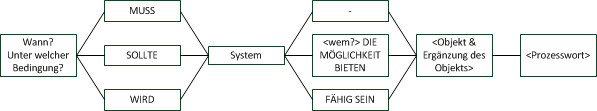
\includegraphics[scale=0.95]{images/anforderungen/satzschablone.png}
\caption[Satzschablone]{Satzschablone (Grafik entnommen aus \cite{req_eng_book})}
\label{fig:satzschablone}
\end{figure}


\newpage
\FloatBarrier
\subsubsection{Funktionale Anforderungen}\label{func_anforderungen}

\begin{table}[ht]
\centering
  \begin{tabular}{ l | p{8cm} }
	\hline
	\rowcolor{gray}
	\textbf{Bezeichner}&	\textbf{RE-F1}\\ \hline
	\textbf{Priorität} 		&	Must\\ \hline
	\textbf{Anforderungstyp}	&	Funktionale Anforderung\\ \hline
	\textbf{Name} 			&	Bereitstellung der Schnittstellen für Optimierungsprobleme\\ \hline
	\textbf{Use Case} 		&	\nameref{table:use_case_1}\\ \hline
	\textbf{Beschreibung} 	&	Das System muss dem Nutzer die Möglichkeit bieten, die Lösung verschiedener Optimierungsprobleme zu beauftragen.\\ \hline
	\textbf{Begründung} 		&	Die Schnittstellen ist die Anlaufstelle des Nutzers. Er beauftragt das System, eine Berechnung zu starten.\\ \hline
	\textbf{Akzeptanz Kriterium}	&	\begin{enumerate}
					\item Der Nutzer kann eine Schnittstelle für die bereitgestellten Berechnungsfunktionen ansprechen.
					\end{enumerate}
					\\ \hline
	\textbf{Abhängigkeiten} 	&	-\\ \hline
  \end{tabular}
   \caption{Anforderung RF-F1}\label{table:req_1}
\end{table}

\begin{table}[ht]
\centering
  \begin{tabular}{ l | p{8cm} }
	\hline
	\rowcolor{gray}
	\textbf{Bezeichner}&	\textbf{RE-F2}\\ \hline
	\textbf{Priorität} 		&	Must\\ \hline
	\textbf{Anforderungstyp}	&	Funktionale Anforderung\\ \hline
	\textbf{Name} 			&	Speicherung der Eingabeparameter\\ \hline
	\textbf{Use Case} 		&	\nameref{table:use_case_1}\\ \hline
	\textbf{Beschreibung} 	&	Falls eine Berechnung in Auftrag gegeben wurde, muss das System fähig sein, die Eingabeparameter abzuspeichern.\\ \hline
	\textbf{Begründung} 		&	Die Berechnung wird von einem anderen System ausgeführt. Damit diese auf die Parameter zugreifen können, müssen die Daten persistiert werden.\\ \hline
	\textbf{Akzeptanz Kriterium}	&	\begin{enumerate}
					\item Die Parameter sind persistiert.
					\item Es gibt eine Fehlermeldung, falls bei der Speicherung etwas fehlschlägt oder die Eingabeparameter nicht gültig sind.
					\end{enumerate}
					\\ \hline
	\textbf{Abhängigkeiten} 	&	\\ \hline
  \end{tabular}
   \caption{Anforderung RF-F2}\label{table:req_3}
\end{table}

\begin{table}[ht]
\centering
  \begin{tabular}{ l | p{8cm} }
	\hline
	\rowcolor{gray}
	\textbf{Bezeichner}&	\textbf{RE-F3}\\ \hline
	\textbf{Priorität} 		&	Must\\ \hline
	\textbf{Anforderungstyp}	&	Funktionale Anforderung\\ \hline
	\textbf{Name} 			&	Rückgabe einer ID bei Beauftragung\\ \hline
	\textbf{Use Case} 		&	\nameref{table:use_case_1}\\ \hline
	\textbf{Beschreibung} 	&	Falls eine Berechnung in Auftrag gegeben wurde, muss das System dem Ersteller eine ID zurückliefern.\\ \hline
	\textbf{Begründung} 		&	Die ID hilft dem Nutzer den Status der Berechnung abzuholen und wird am Schluss für das Resultat benötigt.\\ \hline
	\textbf{Akzeptanz Kriterium}	&	\begin{enumerate}
					\item Der Nutzer erhält nach dem Starten einer Berechnung eine ID.
					\end{enumerate}
					\\ \hline
	\textbf{Abhängigkeiten} 	&	\nameref{table:req_3}\\ \hline
  \end{tabular}
   \caption{Anforderung RF-F3}\label{table:req_2}
\end{table}

\begin{table}[ht]
\centering
  \begin{tabular}{ l | p{8cm} }
	\hline
	\rowcolor{gray}
	\textbf{Bezeichner}&	\textbf{RE-F4}\\ \hline
	\textbf{Priorität} 		&	Must\\ \hline
	\textbf{Anforderungstyp}	&	Funktionale Anforderung\\ \hline
	\textbf{Name} 			&	Start der Berechnung\\ \hline
	\textbf{Use Case} 		&	\nameref{table:use_case_2}\\ \hline
	\textbf{Beschreibung} 	&	Falls eine Berechnung in Auftrag gegeben wurde, muss das System fähig sein, die Berechnung beim Verarbeitungssystem zu starten.\\ \hline
	\textbf{Begründung} 		&	Der Nutzer kennt das Verarbeitungssystem nicht, das System muss dem Verarbeitungssystem den Start-Befehl geben.\\ \hline
	\textbf{Akzeptanz Kriterium}	&	\begin{enumerate}
					\item Der Befehl für den Start wird versendet und die ID dabei übergeben.
					\item Die Fehlermeldung bei einem Fehlversuch wird gespeichert.
					\end{enumerate}
					\\ \hline
	\textbf{Abhängigkeiten} 	&	\nameref{table:req_3}\\ \hline
  \end{tabular}
   \caption{Anforderung RF-F4}\label{table:req_4}
\end{table}

\begin{table}[ht]
\centering
  \begin{tabular}{ l | p{8cm} }
	\hline
	\rowcolor{gray}
	\textbf{Bezeichner}&	\textbf{RE-F5}\\ \hline
	\textbf{Priorität} 		&	Must\\ \hline
	\textbf{Anforderungstyp}	&	Funktionale Anforderung\\ \hline
	\textbf{Name} 			&	Abfrage der Eingabeparameter\\ \hline
	\textbf{Use Case} 		&	\nameref{table:use_case_3}\\ \hline
	\textbf{Beschreibung} 	&	Falls eine Berechnung in Auftrag gegeben wurde, muss das System dem Verarbeitungssystem die Möglichkeit bieten, die Eingabeparameter abzufragen.\\ \hline
	\textbf{Begründung}		&	Damit das Verarbeitungssystem die Berechnung durchführen kann, braucht es die Eingabeparameter.\\ \hline
	\textbf{Akzeptanz Kriterium}	&	\begin{enumerate}
					\item Das Verarbeitungssystem erhält die Eingabeparameter.
					\item Das Verarbeitungssystem erhält eine Fehlermeldung, falls keine Eingabeparameter vorhanden sind.
					\end{enumerate}
					\\ \hline
	\textbf{Abhängigkeiten} 	&	\nameref{table:req_3}\\ \hline
  \end{tabular}
   \caption{Anforderung RF-F5}\label{table:req_5}
\end{table}

\begin{table}[ht]
\centering
  \begin{tabular}{ l | p{8cm} }
	\hline
	\rowcolor{gray}
	\textbf{Bezeichner}&	\textbf{RE-F6}\\ \hline
	\textbf{Priorität} 		&	Should\\ \hline
	\textbf{Anforderungstyp}	&	Funktionale Anforderung\\ \hline
	\textbf{Name} 			&	Abfrage des Status\\ \hline
	\textbf{Use Case} 		&	\nameref{table:use_case_4}\\ \hline
	\textbf{Beschreibung} 	&	Falls eine Berechnung in Auftrag gegeben wurde, sollte das System dem Nutzer die Möglichkeit bieten, den Status der Berechnung abzufragen.\\ \hline
	\textbf{Begründung} 		&	Da die Verarbeitung asynchron läuft, weiss der Benutzer nicht, wann seine Berechnung fertig ist.\\ \hline
	\textbf{Akzeptanz Kriterium}	&	\begin{enumerate}
					\item Der Nutzer erhält einen Status seiner Berechnung.
					\end{enumerate}
					\\ \hline
	\textbf{Abhängigkeiten} 	&	\nameref{table:req_2}\\ \hline
  \end{tabular}
   \caption{Anforderung RF-F6}\label{table:req_6}
\end{table}

\begin{table}[ht]
\centering
  \begin{tabular}{ l | p{8cm} }
	\hline
	\rowcolor{gray}
	\textbf{Bezeichner}&	\textbf{RE-F7}\\ \hline
	\textbf{Priorität} 		&	Nice to have\\ \hline
	\textbf{Anforderungstyp}	&	Funktionale Anforderung\\ \hline
	\textbf{Name} 			&	Registrierung eines WebHooks für Statusänderungen\\ \hline
	\textbf{Use Case} 		&	\nameref{table:use_case_4}\\ \hline
	\textbf{Beschreibung} 	&	Falls eine Berechnung in Auftrag gegeben und dazu ein WebHook eingetragen wurde, sollte das System den Nutzer über eine Änderung des Status mittels 
						WebHook informieren.\\ \hline
	\textbf{Begründung} 		&	Da die Verarbeitung asynchron läuft, weiss der Benutzer nicht, wann seine Berechnung fertig ist. Um ein ständiges Pollen zu vermeiden, können 
							WebHooks verwenden werden.\\ \hline
	\textbf{Akzeptanz Kriterium}	&	\begin{enumerate}
					\item Der Nutzer wird über die Änderung des Status auf dem eingetragen WebHook informiert.
					\end{enumerate}
					\\ \hline
	\textbf{Abhängigkeiten} 	&	\nameref{table:req_2}\\ \hline
  \end{tabular}
   \caption{Anforderung RF-F7}\label{table:req_7}
\end{table}

\begin{table}[ht]
\centering
  \begin{tabular}{ l | p{8cm} }
	\hline
	\rowcolor{gray}
	\textbf{Bezeichner}&	\textbf{RE-F8}\\ \hline
	\textbf{Priorität} 		&	Must\\ \hline
	\textbf{Anforderungstyp}	&	Funktionale Anforderung\\ \hline
	\textbf{Name} 			&	Speicherung des Resultats\\ \hline
	\textbf{Use Case} 		&	\nameref{table:use_case_5}\\ \hline
	\textbf{Beschreibung} 	&	Nach der Berechnung muss das System dem Verarbeitungssystem die Möglichkeit bieten, das Resultat abspeichern zu können.\\ \hline
	\textbf{Begründung} 		&	Das Resultat muss, bis der Nutzer es abholt, zwischengespeichert werden.\\ \hline
	\textbf{Akzeptanz Kriterium}	&	\begin{enumerate}
					\item Das Verarbeitungssystem kann das Resultat abspeichern.
					\item Das Verarbeitungssystem erhält eine Fehlermeldung, falls das Speichern fehlgeschlagen ist.
					\end{enumerate}
					\\ \hline
	\textbf{Abhängigkeiten} 	&	\nameref{table:req_4}\\ \hline
  \end{tabular}
   \caption{Anforderung RF-F8}\label{table:req_8}
\end{table}

\begin{table}[ht]
\centering
  \begin{tabular}{ l | p{8cm} }
	\hline
	\rowcolor{gray}
	\textbf{Bezeichner}&	\textbf{RE-F9}\\ \hline
	\textbf{Priorität} 		&	Must\\ \hline
	\textbf{Anforderungstyp}	&	Funktionale Anforderung\\ \hline
	\textbf{Name} 			&	Abfrage des Resultats\\ \hline
	\textbf{Use Case} 		&	\nameref{table:use_case_6}\\ \hline
	\textbf{Beschreibung} 	&	Das System muss dem Nutzer die Möglichkeit bieten, das Resultat der Berechnung abzufragen.\\ \hline
	\textbf{Begründung} 		&	Der Nutzer möchte das Resultat der Berechnung wissen.\\ \hline
	\textbf{Akzeptanz Kriterium}	&	\begin{enumerate}
					\item Der Nutzer erhält das Resultat der Berechnung.
					\item Der Nutzer erhält eine entsprechende Fehlermeldung, wenn beim Bereitstellen des Resultats ein Fehler aufgetreten ist.
					\end{enumerate}
					\\ \hline
	\textbf{Abhängigkeiten} 	&	\nameref{table:req_2}\\ \hline
  \end{tabular}
   \caption{Anforderung RF-F9}\label{table:req_9}
\end{table}

\newpage
\FloatBarrier
\subsubsection{Qualitätsanforderung}\label{non_func_anforderungen}

\begin{table}[ht]
\centering
  \begin{tabular}{ l | p{8cm} }
	\hline
	\rowcolor{gray}
	\textbf{Bezeichner}&	\textbf{RE-NF1}\\ \hline
	\textbf{Priorität} 		&	Should\\ \hline
	\textbf{Anforderungstyp}	&	Qualitätsanforderung\\ \hline
	\textbf{Name} 			&	Prozess-agnostische Schnittstelle\\ \hline
	\textbf{Use Case} 		&	\nameref{table:use_case_1}\\ \hline
	\textbf{Beschreibung} 	&	Das System sollte fähig sein, die Lösung eines Problems so bereitzustellen, dass kein Wissen über den Verarbeitungsprozess erforderlich ist.\\ \hline
	\textbf{Begründung} 		&	Der Verarbeitungsprozess kann spezifisch und von Problem zu Problem unterschiedlich sein, der Nutzer sollte eine möglichst einfache 
							Schnittstelle dafür haben.\\ \hline
	\textbf{Akzeptanz Kriterium}	&	\begin{enumerate}
					\item Das Interface kann verwendet werden, ohne dass das Verarbeitungssystem bekannt ist.
					\end{enumerate}
					\\ \hline
	\textbf{Abhängigkeiten} 	&	-\\ \hline
  \end{tabular}
   \caption{Qualitätsanforderung RF-NF1}\label{table:req_nf_1}
\end{table}

\begin{table}[ht]
\centering
  \begin{tabular}{ l | p{8cm} }
	\hline
	\rowcolor{gray}
	\textbf{Bezeichner}&	\textbf{RE-NF2}\\ \hline
	\textbf{Priorität} 		&	Should\\ \hline
	\textbf{Anforderungstyp}	&	Qualitätsanforderung\\ \hline
	\textbf{Name} 			&	Entgegennahme generischer Eingabeparameter\\ \hline
	\textbf{Use Case} 		&	\nameref{table:use_case_1}\\ \hline
	\textbf{Beschreibung} 	&	Das System sollte in der Lage sein, unterschiedliche Ausprägungen von Eingabeparametern entgegenzunehmen.\\ \hline
	\textbf{Begründung} 		&	Da es bei den Problemen unterschiedliche Ausprägungen gibt, ist auf eine generische Deserialisierung der Eingabeparameter hinzuarbeiten.\\ \hline
	\textbf{Akzeptanz Kriterium}	&	\begin{enumerate}
					\item Unterschiedliche Ausprägungen eines Problems benutzen die gleiche API.
					\end{enumerate}
					\\ \hline
	\textbf{Abhängigkeiten} 	&	-\\ \hline
  \end{tabular}
   \caption{Qualitätsanforderung RF-NF2}\label{table:req_nf_2}
\end{table}

\begin{table}[ht]
\centering
  \begin{tabular}{ l | p{8cm} }
	\hline
	\rowcolor{gray}
	\textbf{Bezeichner}&	\textbf{RE-NF3}\\ \hline
	\textbf{Priorität} 		&	Should\\ \hline
	\textbf{Anforderungstyp}	&	Qualitätsanforderung\\ \hline
	\textbf{Name} 			&	Speicherung generischer Eingabeparameter\\ \hline
	\textbf{Use Case} 		&	\nameref{table:use_case_1}\\ \hline
	\textbf{Beschreibung} 	&	Das System sollte Eingabeparameter einheitlich abspeichern.\\ \hline
	\textbf{Begründung} 		&	Da es viele unterschiedliche Probleme gibt, ist eine generische Persistierung anzustreben.\\ \hline
	\textbf{Akzeptanz Kriterium}	&	\begin{enumerate}
					\item Unterschiedliche Probleme haben kein abweichendes Persistierungsschema.
					\end{enumerate}
					\\ \hline
	\textbf{Abhängigkeiten} 	&	-\\ \hline
  \end{tabular}
   \caption{Qualitätsanforderung RF-NF3}\label{table:req_nf_3}
\end{table}

\newpage
\subsection{Zusammenfassung der Anforderungen}\label{toc_anfoderungen}
Die Priorität der einzelnen Anforderungen ist wichtig, falls nicht alle Anforderungen umgesetzt werden können. Die Priorität wurde zusammen mit den \glslink{stakeholder}{Stakeholdern} 
festgelegt und in \autoref{table:req_priorities} zur besseren Übersicht zusammengetragen.
\begin{table}[ht]
\centering
  \begin{tabular}{ l | l | l }
	\hline
	\rowcolor{gray}
	\textbf{Bezeichner}	& \textbf{Name}	&	\textbf{Priorität}\\ \hline
	RE-F1 			&  Bereitstellung der Schnittstellen für Optimierungsprobleme	& Must\\ \hline
	RE-F2 			&  Speicherung der Eingabeparameter	& Must\\ \hline
	RE-F3 			&  Rückgabe einer ID bei Beauftragung	& Must\\ \hline
	RE-F4 			&  Start der Berechnung	& Must\\ \hline
	RE-F5 			&  Abfrage der Eingabeparameter	& Must\\ \hline
	RE-F6 			&  Abfrage des Status	& Should\\ \hline
	RE-F7 			&  Registrierung eines WebHooks für Statusänderungen	& Nice to have\\ \hline
	RE-F8 			&  Speicherung des Resultats	& Must\\ \hline
	RE-F9 			&  Abfrage des Resultats	& Must\\ \hline
	RE-NF1 			&  Prozess-agnostische Schnittstelle & Should\\ \hline
	RE-NF2 			&  Entgegennahme generischer Eingabeparameter & Should\\ \hline
	RE-NF3 			&  Speicherung generischer Eingabeparameter & Should\\ \hline
  \end{tabular}
   \caption{Priorität der Anforderungen}\label{table:req_priorities}
\end{table}
%%%%%%%%%%%%%%%%%%%%%%%%%%%%%%%%%%%%%%%%%%%%%%%%%%%%%%%%%%%%%%%%%
%
% Project     : Bachelorarbeit
% Title       : Machbarkeitsanalyse für eine ressourcenorientierte Schnittstelle zur Verarbeitung grundlegender Probleme der Informatik
% File        : architektur.tex Rev. 01
% Date        : 01.03.2015
% Author      : Raffael Santschi
%
%%%%%%%%%%%%%%%%%%%%%%%%%%%%%%%%%%%%%%%%%%%%%%%%%%%%%%%%%%%%%%%%%

\chapter{Konzept der Schnittstelle \resultAssignment{[R4]}}\label{chap.architektur}
In diesem Kapitel wird auf die Strukur und das Konzept der Schnittstelle eingegangen. Dieses Konzept legt die Grundlage für die Umsetzung und entscheidet somit, ob die 
Aufgabe gelöst werden kann.

\section{Übersicht}\label{architektur_uebersicht}
Die Systemumgebung (siehe Abbildung \ref{fig:system_scope}) hat zwei Berührungspunkte zur Aussenwelt. Der eine ist zum Nutzer hin, der andere zu einem Verarbeitungssystem. 
Um die Daten zu speichern, wird eine Datenbank benötigt. Das ermöglicht einen asynchronen Ablauf und ein mehrfaches Abfragen der Daten.
\begin{figure}[h]
\centering
\includegraphics[scale=0.8]{images/visio/SystemScope.png}
\caption[System Übersicht]{System Übersicht \selfmade{}}
\label{fig:system_scope}
\end{figure}

\section{Konzept}\label{arch_backend}
Das Konzept sollte simpel und flexibel sein, damit das System möglichst schnell erweitert werden kann. Beim Betrachten der Probleme und der Abläufe wurde bemerkt, dass die Vorgänge 
Ähnlichkeiten aufweisen. Die Daten werden angenommen und für einen bestimmten Algorithmus aufbereitet. Das Verarbeitungssystem schickt das Resultat zurück und dieses wird dann 
wieder umgewandelt, so dass es für den Nutzer brauchbar ist. Es finden zwei Umwandlungen statt. Die Umwandlungen an sich sind von Problem zu Problem verschieden, jedoch gibt es 
auch dort gewisse Ähnlichkeiten. In \autoref{fig:architektur} wird der Aufbau des System gezeigt. Die  \gls{domainlanguage} des Nutzers wird mit Hilfe der Controller, Entities und 
den Translators auf die \gls{domainlanguage} der Algorithmen abgebildet.

\begin{figure}[h]
\centering
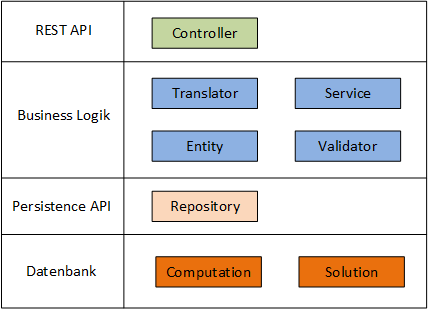
\includegraphics[scale=0.8]{images/visio/architektur_db.png}
\caption[Architekturaufbau des Systems]{Architekturaufbau des Systems \selfmade{}}
\label{fig:architektur}
\end{figure}
 
\FloatBarrier
\subsection{REST API}
Für die Schnittstelle wird ein \gls{rest} \gls{api} erstellt, welches die nötigen Funktionen bietet. Das \gls{api} funktioniert nach dem De-facto-Standard 
(siehe \cite{wiki_restful}). Falls Fehler auftreten, werden die \gls{http_statuscode} verwendet, um diese an den Aufrufer weiterzugeben.

\subsection{Business Logik}
Die Business Logik besteht aus Translator, Service, Entity und Validator von den jeweiligen Problemen. 
\paragraph{Translator}
Es gibt jeweils ein `ComputationTranslator' für die Umwandlung vom Nutzer hin zum Algorithmus und einen `SolutionTranslator' für die Umwandlung vom Algorithmus zurück in das System. In den 
Translators steckt die ganze Logik. Hier fliesst ein, wie der Algorithmus die Daten für die Verarbeitung benötigt und wie das Resultat zurück kommt. Es wäre zum Beispiel möglich, die Daten in 
Kombinationen für einen evolutionären Algorithmus umzuwandeln, so würde allenfalls ein generischer Algorithmus für alle Probleme ausreichen. Ebenfalls möglich wäre eine Umwandlung des 
Stundenplanproblems auf ein Knotenfärbungsproblem und somit könnte der gleiche Algorithmus angesprochen werden (vergleiche \cite{timetabling_abdullah}). Die Möglichkeiten mit dem 
Konzept der Translators ist sehr vielfälltig. Zusätzlich kann im Translator das Resultat mit zusätzlichen Informationen, zum Beispiel Statistiken, angereichert werden.
\paragraph{Service}
Der Service kann sehr generisch gehalten werden und benötigt keine problemspezifisches Methoden. 
\paragraph{Entity}
Die Entitäten sind von Problem zu Problem unterschiedlich. Es muss analysiert werden, wie die Parameter am besten eingegeben werden und wie diese dann vom Algorithmus 
gebraucht werden. 
\paragraph{Validator}
Der Validator entscheidet, ob eine Lösung gültig ist oder nicht. Wie bereits im \autoref{cat_theo_inf} erklärt, kann jedes NP-vollständige Problem in \glslink{polynomialzeit}{polynomialer} Zeit validiert werden.

\subsection{Persistance API}
Die Abstraktion der Datenbank wird mittels eines Persistance APIs, welches mit der Datenbank interagiert, realisiert. Dieses API ist für das Laden und Speichern der Daten 
verantwortlich und bietet die Möglichkeit, spezifische Abfragen auszuführen.

\subsection{Datenbank}
Jedes Problem hat seine eigene Ausprägung von Computation und Solution, welche abgespeichert werden müssen. Die Datenbank sollte, wenn möglich, eine ähnliche Flexibilität, wie 
das Programm selber, aufweisen. Die Vorgänge benötigen keine Transaktionen und sind zum grossen Teil nur Einfüge-Operationen, nur selten wird ein Eintrag geändert. Die Daten werden 
immer in der Nutzer-Sicht gespeichert.

\begin{landscape}
\subsection{Ablauf}
\thispagestyle{empty}
In \autoref{fig:workflow} wird der Ablauf des ganzen Vorganges und die Interaktion mit dem Nutzer und dem Verarbeitungssystem verdeutlicht. Die Translators, welche in dem 
Prototyp verwendet werden, sind nur eine Möglichkeit, welche dieses Konzept bietet. Generell baut dieses Konzept auf eine pre- und post-Aktion vor bzw. nach dem Starten des Algorithmus 
auf.

\begin{figure}[h]
\centering
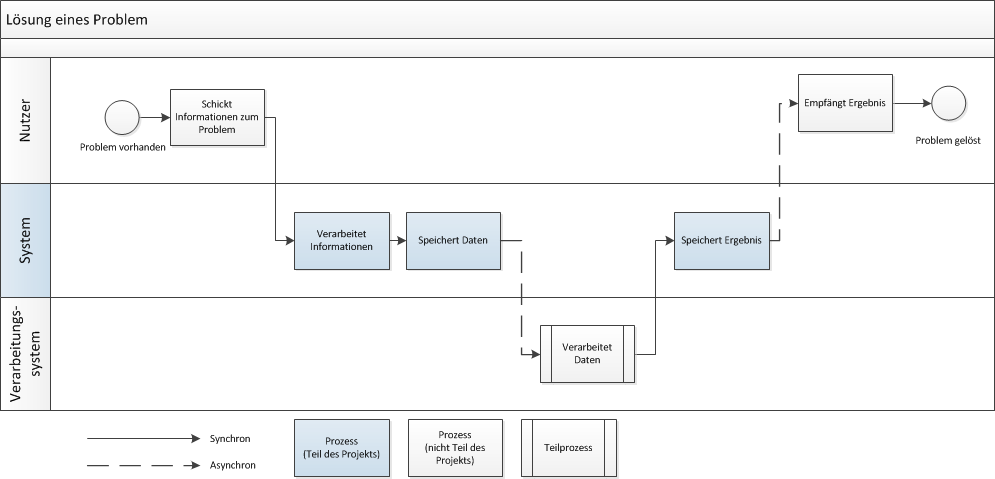
\includegraphics[scale=0.8]{images/visio/workflow.png}
\caption[Flussdiagramm des Arbeitsablaufs]{Flussdiagramm des Arbeitsablaufs \selfmade{}}
\label{fig:workflow}
\end{figure}

\end{landscape}

Die \autoref{fig:sequenz_diagramm_start} zeigt das Sequenzdiagramm für den Start eines beliebigen Problems, alle Komponenten mit '\{Problem\}' sind spezifische Problem-Komponenten, 
die anderen sind generische. Bei Speichern einer Berechnung wird der Status 'CREATED' gesetzt. Nach dem Speichern wird über die `Solver'-Komponente asynchron das Verarbeitungssystem 
gestartet und der Status auf 'STARTED' gesetzt. Das Verarbeitungssystem holt sich die benötigten Informationen. Der Controller lädt das Problem vom Service, dieser wiederum lädt es vom 
Repository und wandelt es für den Algorithmus um.

\begin{figure}[h]
\centering
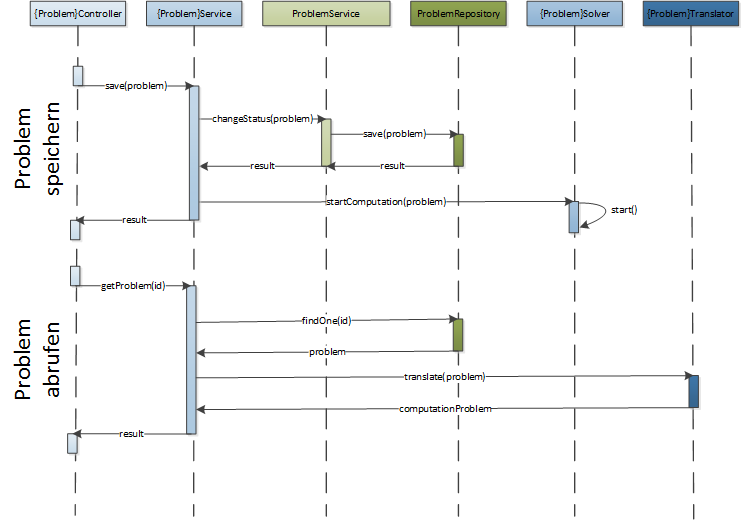
\includegraphics[scale=0.74]{images/visio/sequenz_diagramm_start.png}
\caption[Start eines beliebigen Problemes]{Start eines beliebigen Problemes \selfmade{}}
\label{fig:sequenz_diagramm_start}
\end{figure}

\newpage

Die \autoref{fig:sequenz_diagramm_result} zeigt das Sequenzdiagramm für das Abspeichern eines Resultates einer beliebigen Berechnung. Bei einem Speicheraufruf wird zuerst das Problem 
geladen, danach wird die Lösung vom Algorithmus mit Hilfe der Eingabeparameter transferiert und vom Validator validiert. Nun wird anhand des Resultattypes der Status der Berechnung 
abgeändert. Das Resultat wird mit dem Ergebnis der Validierung in die Datenbank gespeichert. Wenn der Nutzer den Status einer Berechnung abruft, fragt der Controller über den 
Service den Status ab. Der Service lädt das Problem, fragt die vorhandenen Resultate ab, fügt diese zu einem Status zusammen und schickt den Status an den Controller zurück.

\begin{figure}[h]
\centering
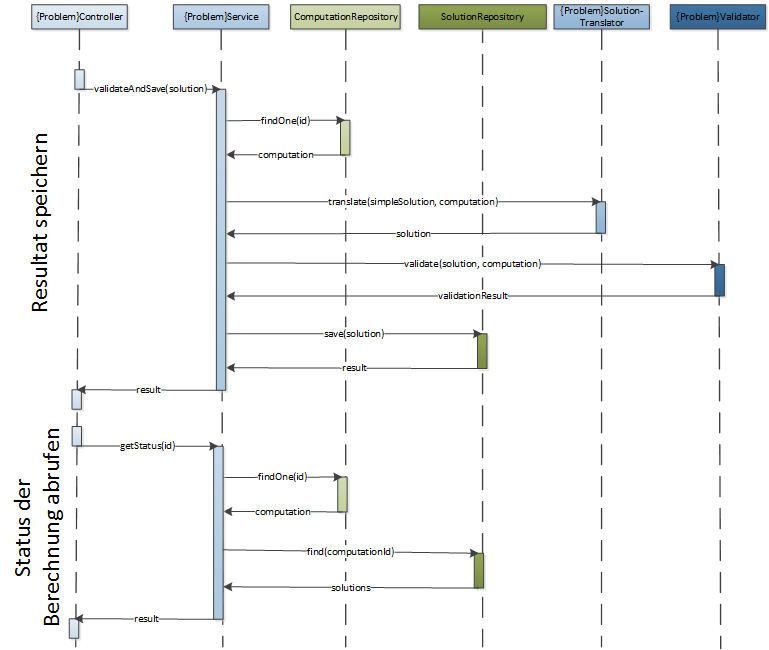
\includegraphics[scale=0.72]{images/visio/sequenz_diagramm_result.png}
\caption[Abspeichern des Resultates eines beliebigen Problemes]{Abspeichern des Resultates eines beliebigen Problemes \selfmade{}}
\label{fig:sequenz_diagramm_result}
\end{figure}

\section{Datenbank Varianten}\label{db_varianten}
Es gibt verschiedene Datenbanktypen und jede hat seine Vor- und Nachteile. In diesem Abschnitt werden vier verschiedenen Typen miteinander verglichen und der beste für diesen 
Anwendungszweck ausgewählt. Um die Eigenheiten der Datenbanken hervorzuheben, wird bei jeder Art das gleiche Beispiel mit der spezifischen Definitions-- und Abfragesprache gemacht.

\subsection{CAP-Theorem}\label{cap_theorem}
Das CAP-Theorem ist im Jahr 2000 aus einer Vermutung von Eric Brewer entstanden \cite{cap_brewer}. Das Theorem zeigt, dass die Werte Konsistenz (C), Verfügbarkeit (A) und Partitionstoleranz (P) ein 
Dreieck (siehe \autoref{fig:cap}) bilden und dass ein verteiltes System nur jeweils zwei dieser Eigenschaften gleichzeitig erfüllen kann.

\begin{figure}[h]
\centering
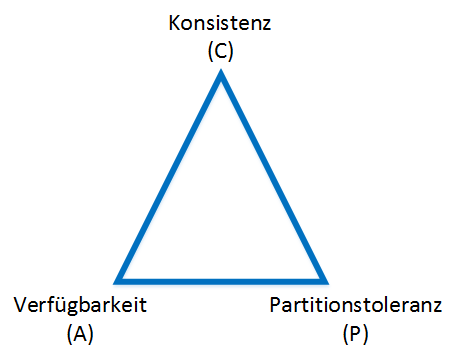
\includegraphics[scale=0.8]{images/visio/cap.png}
\caption[CAP-Theorem]{CAP-Theorem \selfmade{}}
\label{fig:cap}
\end{figure}

\subsubsection{Beispiele}

\begin{itemize}
	\item \textbf{AP}: Domain Name System (DNS), NoSQL Datenbanken
	\item \textbf{CA}: Relationalen Datenbanken
	\item \textbf{CP}: Banken Anwendungen
\end{itemize}

\subsection{Relationales Datenbanksystem}\label{rdbms}
Die Vorteile einer \gls{rdbms} sind die Transaktionen und das dazugehörige \gls{acid} Prinzip (vergleiche \cite{limited2010introduction}). 
\begin{itemize}
	\item \textbf{Atomicity}: Eine Reihe von Befehlen wird entweder ganz oder gar nicht ausgeführt.
	\item \textbf{Consistency}: Der Datenzustand ist nach jeder Veränderung wieder konsistent, wenn dies auch vorher der Fall war.
	\item \textbf{Isolation}: Unterschiedliche Befehlsketten beeinflussen sich nicht gegenseitig.
	\item \textbf{Durability}: Vollzogene Änderungen sind dauerhaft, auch bei einem Systemfehler.
\end{itemize}
Beziehungen zwischen Tabellen werden mit Fremdschlüssel definiert, welche auf einen Hauptschlüssel der zu referenzierenden Tabelle zeigt. \autoref{lst:table_definition_rdbms} zeigt die
Tabelle 'Person', welche eine Verbindung zur Tabelle 'Address' hat.

\begin{lstlisting}[language=SQL, caption=Tabellendefinition in relationalem Datenbanksystem, label=lst:table_definition_rdbms]  
    CREATE TABLE ADDRESS(
             ID       INTEGER(11),
             Street   VARCHAR(30),
             Zip      INTEGER(6),
             City     VARCHAR(12));

    CREATE TABLE PERSON(
               ID          INTEGER(11),
               Name        VARCHAR(50),
               FK_Address  INTEGER(11));
\end{lstlisting}

Die Abfrage der Strasse bei einer relationaler Datenbank mittels \gls{sql} ist in \autoref{lst:select_street_rdbms} dargestellt.

\begin{lstlisting}[language=SQL, caption=Abfrage in relationalem Datenbanksystem, label=lst:select_street_rdbms]  
    SELECT ADDRESS.Street
    FROM PERSON 
    JOIN ADDRESS on PERSON.FK_Address = ADDRESS.ID;
    WHERE PERSON.Name = 'Thomas';
\end{lstlisting}

\subsection{Objektrelationales Datenbanksystem}\label{ordbms}
\glslink{ordbms}{Objektrelationale Datenbankmanagementsysteme (ORDBMS)} wurden entwickelt um, das relationale System mit den Funktionen des objektorientierten Stiles zu erweitern.
Die folgenden Beschreibung der Eigenschaften sind aus \cite{limited2010introduction} abgeleitet. In objektrelationalen Datenbanksystemen werden 
komplexe Datentypen unterstützt, so können zusätzliche Typen definiert werden und diese können dann bei einer Tabellendefinition verwendet werden.  
In \autoref{lst:type_definition_ordbms} ist eine Typendefinition von 'AddressType' zu sehen, welche wiederum in \autoref{lst:use_type_definition_ordbms} 
in der Tabelle 'Person' verwendet wird.

\begin{lstlisting}[language=SQL, caption=Typendefinition in objektrelationalem Datenbanksystem, label=lst:type_definition_ordbms]  
    CREATE TYPE AddressType  AS
             (Street   VARCHAR(30),
              Zip      INTEGER(6),
              City     VARCHAR(12));
\end{lstlisting}

\begin{lstlisting}[language=SQL, caption=Verwendung von Typendefinition in objektrelationalem Datenbanksystem, label=lst:use_type_definition_ordbms]  
    CREATE TABLE PERSON(
               ID       VARCHAR(20),
               Name     VARCHAR(50),
               Address  AddressType);
\end{lstlisting}

Wenn nun die Strasse einer bestimmten Person abgefragt werden möchte, sieht dies in einer objektrelationaler Datenbank wie in \autoref{lst:select_street_ordbms} aus.

\begin{lstlisting}[language=SQL, caption=Abfrage in objektrelationalem Datenbanksystem, label=lst:select_street_ordbms]  
    SELECT Address.Street
    FROM PERSON;
    WHERE Name = 'Thomas';
\end{lstlisting}

Zusätzlich können auch Arrays von Typen definiert werden, in \autoref{lst:use_array_ordbms} ist die Definition der Tabelle 'Person' mit 
bis zu fünf E-Mail-Adressen gezeigt.

\begin{lstlisting}[language=SQL, caption=Verwendung von Array in objektrelationalem Datenbanksystem, label=lst:use_array_ordbms]  
    CREATE TABLE PERSON(
               ID       VARCHAR(20),
               Name     VARCHAR(50),
               Mail     VARCHAR(40) ARRAY[5]);
\end{lstlisting}

Weiter bieten die Systeme die Möglichkeiten, Methoden auf Typen und Tabellen und Vererbungshierarchien zu definieren. Der Anwendungsbereich 
liegt bei Applikationen, welche viele kurzlebige Transaktionen mit komplexen Objekten durchführen.

\subsection{Objekorientiertes Datenbanksystem}\label{object_db}
Das Ziel einer \gls{oodbms} ist eine bessere und nähere Zusammenarbeit mit objektorientierten Sprachen.
Die Informationen über \gls{oodbms} sind aus \cite{limited2010introduction} entnommen. Der grosse Unterschied zu anderen Datenbanksystemen
ist die Persistierung, bei \gls{oodbms} wird bereits beim Erstellen eines neuen persistenten Objekts im Code ein Pointer auf das Objekt in der Datenbank zurückgegeben. 
Weiter unterstützen die Systeme Versionierung von Objekten, die Datenbank kann somit mit verschiedenen Versionen der Objekte gleichzeitig umgehen. 
Dies kann bei einem geplanten Umstrukturierung sehr hilfreich sein, wenn die neue Version erst für Tests verwendet wird und die bestehenden Objekte erst nach dem 
Release migriert werden sollen. \autoref{lst:table_definition_oodbms} zeigt, wie das Objekt 'Person' in \gls{odl} definiert wird.

\begin{lstlisting}[language=C++, caption=Objektdefinition in objektorientierem Datenbanksystem, label=lst:table_definition_oodbms]  
    class PERSON
    {
          attribute string Id;
          attribute string Name;
          attribute struct Address
              { string Street,
                short Zip,
                string City} address;
    }
\end{lstlisting}

Für die Abfrage der Strasse einer Person wird ein Statement wie in \autoref{lst:select_street_oodbms} verwendet. Diese Abfragesprache nennt
sich \gls{oql}. Die Attribute der Objekte und Structs können mit einem Punkt separiert verkettet werden.

\begin{lstlisting}[language=SQL, caption=Abfrage in objektorientierem Datenbanksystem, label=lst:select_street_oodbms]  
    SELECT p.Address.Street
    FROM persons p
    WHERE p.Name = 'Thomas';
\end{lstlisting}

Die objektorientierten Datenbanksystemen bietet die aus den \gls{rdbms} bekannten Abfragefunktionen (Avg, Max, Min, Distinct). 
Zuätzlich können bei diesen Systemen Vererbungshierarchien und Methoden in Objekten definiert werden. Sie werden bei Applikationen verwendet,
welche oft und lange mit komplexen Objekten arbeiten.

\subsection{NoSQL Datenbanksystem}\label{no_sql_db}
NoSQL Datenbanksysteme folgen nicht dem \gls{acid} Prinzip, sie sind entwickelt worden, um den erforderlichen Geschwindigkeiten und Grössen von Anwendungen wie Google, 
Facebook, Yahoo und Twitter zu genügen. Die Systeme sind nicht relational aufgebaut und verwenden oft eine andere Abfragesprache als \gls{sql} (siehe \cite{vaish2013getting}). 
Die meisten NoSQL Datenbanksystem setzen auf das \gls{base}-Prinzip von Eric Brewer.

\begin{myQuote}{Gaurav Vaish \cite{vaish2013getting}}
"`\textbf{Basic availability}: Each request is guaranteed a response—successful or failed execution.\\
\textbf{Soft state}: The state of the system may change over time, at times without any input (for eventual consistency).\\
\textbf{Eventual consistency}: The database may be momentarily inconsistent but will be consistent eventually."'
\end{myQuote}

Nahe zu alle NoSQL Datenbanksysteme sind schemalos, dass heisst, die Tabellen müsse nicht im Vorherein definiert werden. Die Abfragen gestalten sich einfach, JOIN Befehle entfallen 
komplett. Durch den lockeren Aufbau kann eine höhere Performance erzielt werden, die Unterschiede bei der Geschwindigkeit werden bereits bei kleineren Datenmengen bemerkbar.

\subsubsection{NoSQL Datenbanktypen}\label{no_sql_db_subgroups}
NoSQL ist eine Übergruppe von unterschiedlichen Datenbanktypen. In diesem Abschnitt wird auf drei verschiedene NoSQL Datenbanktypen eingegangen, die Eigenschaften der jeweiligen
 Typen sind aus \cite{vaish2013getting} entnommen.

\paragraph{Document}
Bei dokumentorientierten Datenbanken werden \gls{semi_structured_data} abgespeichert, diese verwenden meistens die Dateiformate \gls{json}, 
\gls{xml} oder \gls{yaml}. Die meisten Datenbanksysteme dieser Art haben kein definiertes Schema für Einträge oder 
nur ein teilweise definiertes Schema. Es ist somit möglich ganz unterschiedliche Elemente in eine Tabelle bzw. Collection, so werden Tabellen in dieser Welt genannt, zu speichern. Diese Erklärung 
erinnert an \gls{blob} in relationalen Datenbanken, jedoch können hier Indexes auf bestimmte Attribute gesetzt und innerhalb der Elemente effizient gesucht 
werden.

In \autoref{lst:person_mongodb} wird ein Personen Element gezeigt, welches in der Collection 'Persons' gespeichert ist. Dieses Beispiel ist basierend auf einer MongoDB Instanz, die Definition 
für die Collection entfällt komplett.

\begin{lstlisting}[language=JSON, caption=Personen Element in JSON Format, label=lst:person_mongodb]  
    {
       _id: 1,
       name: "Thomas",
       address: {
                 street: "Bahnhofstrasse 45",
                 zip: 8315,
                 city: "Lindau"}
    }
\end{lstlisting}

\autoref{lst:select_mongodb} zeigt die Abfrage der Strasse bei MongoDB, welche das Resultat aus \autoref{lst:select_result_mongodb} liefert. Bei MongoDB wird bei einer Abfrage standardmässig 
immer das ganze Element zurückgegeben, falls nur gewiese Attribute abgefragt werden sollen, können diese in dem Projektionsabschnitt definiert werden. Die ID des Elements wird, so lang 
sie nicht explizit ausgeschlossen wird, immer mit selektiert.

\begin{lstlisting}[language=SQL, caption=Abfrage in MongoDB, label=lst:select_mongodb]  
    db.persons.find({name: "Thomas"}, {_id: 0, "address.street": 1})
\end{lstlisting}

\begin{lstlisting}[language=JSON, caption=Resultat der Abfrage in MongoDB, label=lst:select_result_mongodb]  
    {
       address: {
                 street: "Bahnhofstrasse 45"}
    }
\end{lstlisting}

\paragraph{Column-oriented}
Anders als bei relationalen Datenbanken, welche zeilenorientierte sind, werden die Daten spaltenorientiert gespeichert. Eine Lohndatenbank würde serialisiert beim zeilenorientierten Konzept
wie in \autoref{lst:ser_rowbased_db} und beim spaltenorientierten Ansatz wie in \autoref{lst:ser_columnbased_db} aussehen.

\begin{lstlisting}[language=SQL, caption=Serialisierung zeilenorientierte Datenbank, label=lst:ser_rowbased_db]  
    1,Thomas,100000
    2,Patrick,120000
    3,Andreas,200000
\end{lstlisting}

\begin{lstlisting}[language=SQL, caption=Serialisierung spaltenorientierte Datenbank, label=lst:ser_columnbased_db]  
    1,2,3
    Thomas,Patrick,Andreas
    100000,120000,200000
\end{lstlisting}

Die Definitions- und Abfragesprache ist gleich wie bei relationalen Datenbanken, deshalb wird hier auf Beispiele verzichtet. Der Vorteil 
einer spaltenorientierten Datenbank liegt in der Performance bei \glspl{aggregationsfunktion}. Weiter führt dieser Datenbanktyp Veränderungen, 
welche alle Werte einer Spalte betreffen, effizient durch. Dafür ist das Einfügen einer neu Zeile oder das Auslesen einer ganze Zeile aufwendiger als bei dem zeilenorientierten Ansatz.

\paragraph{Graph}
In Graphdatenbanken sind die abgespeicherten Objekte die Knoten und die Beziehung der Objekte bilden die Kanten. Die Kanten können zusätzlich mit Eigenschaften versehen werden. Dieser 
Datenbanktyp kann für komplexe Netzwerke verwendet werden. Der Vorteil liegt bei der Handhabung der Beziehungen. Das Herausfinden der kürzesten Route zwischen zwei Elementen über 
ihre definierten Beziehungen stellt für diesen Datenbanktyp keine Herausforderung dar.

Die Daten werden je nach Implementation auch in Dokumenten abgespeichert, somit entfällt auch hier eine Definition des Schemas. In \autoref{lst:select_neo4j} ist das Beispiel 
für das Abfragen der Strasse einer Person in Neo4j zu sehen.

\begin{lstlisting}[language=SQL, caption=Abfrage in Neo4j, label=lst:select_neo4j]  
       MATCH (person:Person)
       WHERE person.name = "Thomas"
       RETURN person.address.street;
\end{lstlisting}

\subsection{Vorselektierung}\label{preselection}
Um nicht alle sechs vorgestellten Datenbanksysteme in der Nutzwertanalyse miteinander vergleichen zu müssen, wurde eine Vorselektierung aufgrund der Ist-Analyse gemacht. Da 
objektrelationalen und objektorientierte Datenbanksystem eher akademischer Natur sind und keine detailierte Dokumentation darüber gefunden wurde, werden sie von der Nutzwertanalyse 
ausgeschlossen. Die Anforderungen lassen auf keinen Anwendungsfall für eine spaltenorientierte Datenbank schliessen. In den einzelnen Problemen spielen Beziehungen zwischen Objekten 
zwar oft eine Rolle, doch das würde eher in den Bereich des Algorithmus fallen, aus diesem Grund werden Graphdatenbanken ebenfalls ausgeschlossen. Somit bleiben noch die relationale 
Datenbank und die dokumentorientierten Datenbanken für die Nutzwertanalyse übrig.

Da es innerhalb der ausgewählten Datenbanksystemen sehr viele verschiedene Implementationen gibt, wurden von jedem Typ eine ausgewählt. Bei den relationalen Datenbanken fiel die 
Entscheidung auf MySQL, da diese Implementation kostenlos ist und bereits Erfahrung vorhanden war. Da MongoDB sehr verbreitet und eine gute Integration in die Java Frameworks hat, 
wurde diese Implementation unter den dokumentorientierten Datenbanken ausgewählt.

\newpage
\section{Nutzwertanalyse}\label{architektur_nutzwertanalyse}

\subsection{Bewertungskriterien}\label{architektur_bewertungspunkte}

In der Nutzwertanalyse werden folgende Punkte betrachtet und nach dem angegebenen Schema bewertet und dann gewichtet. 
Die Kriterien sind grösstenteils aus den \gls{cap_theorem} abgeleitet.

\paragraph{Aufwand}
\begin{itemize}
	\item \textbf{Beschreibung}: Wie gross ist der geschätzte Aufwand mit dieser Datenbanktyp?
	\item \textbf{Bewertung}: 1: sehr hoch, 10: sehr niedrig
	\item \textbf{Gewichtung}: 5 (Die Zeit für dieses Projekt ist beschränkt und die Entscheidung könnte zu einem Risiko werden.)
\end{itemize}

\paragraph{Änderbarkeit}
\begin{itemize}
	\item \textbf{Beschreibung}: Wie flexibel ist diese Variante in Bezug auf Erweiterungen/Vererbung?
	\item \textbf{Bewertung}: 1: sehr spezifisch, 10: sehr flexibel
	\item \textbf{Gewichtung}: 5 (Die Anforderungen geben vor, dass das System einfach zu erweitern sein sollte.)
\end{itemize}

\paragraph{Konsistenz}
\begin{itemize}
	\item \textbf{Beschreibung}: Wie gut ist die Datenbank in Bezug auf Konsistenz?
	\item \textbf{Bewertung}: 1: gar nicht 10: sehr gut
	\item \textbf{Gewichtung}: 2 (Die Daten haben untereinander so gut wie keine Abhängigkeiten, es werden fast nur Einfüge-Operationen benützt.)
\end{itemize}

\paragraph{Verfügbarkeit}
\begin{itemize}
	\item \textbf{Beschreibung}: Wie hoch ist die Verfügbarkeit der Datenbank Operationen?
	\item \textbf{Bewertung}: 1: niedrig, 10: sehr hoch
	\item \textbf{Gewichtung}: 4 (Die Schnittstelle wird für möglichst viele gleichzeitige Requests ausgelegt, eine Warteschlaufe von Operationen ist nicht gewünscht.)
\end{itemize}

\paragraph{Partitionstoleranz}
\begin{itemize}
	\item \textbf{Beschreibung}: Kann die Datenbank verteilt betrieben werden können?
	\item \textbf{Bewertung}: 1: nur eingeschränkt, 10: sehr einfach
	\item \textbf{Gewichtung}: 4 (Mit zunehmender Grösse wird die Datenbank sehr wahrscheinlich verteilt betrieben.)
\end{itemize}

\newpage
\subsection{Bewertung}\label{architektur_bewertung}
Anhand der zuvor definierten Kriterien wurde eine Bewertung vorgenommen. Diese Bewertung ist nicht generell gültig, sie bezieht sich nur auf dieses Projekt.

\begin{table}[ht]
\centering
  \begin{tabular}{>{\columncolor{darkgray}} l | p{5cm} | p{5cm}}
	\hline
	\rowcolor{darkgray}
	\textbf{Kriterium}		&	\textbf{Relationale Datenbank} 	&	\textbf{Dokumentorientierten Datenbank}	\\ \hline
	\rowcolor{gray}
	Aufwand		&	7 (35)		&	7 (35)		\\ \hline
	Begründung		&	MySQL ist bekannt und das Einrichten ist relativ schnell gemacht.			
				&	Dokumentorientierten Datenbank noch nie benutzt. Laut Informanten ziemlich simpel.	\\ \hline
	\rowcolor{gray}
	Änderbarkeit		&	3 (15)		&	10 (50)		\\ \hline
	Begründung		&	Jede Anpassung an den Entities Attributen erfordert auch eine Änderung des Schemas.
				&	Sehr flexibel, bei Änderungen der Entities oder neuen Probleme keine Anpassung nötig.\\ \hline
	\rowcolor{gray}
	Konsistenz		&	10 (20)	&	4 (8)		\\ \hline
	Begründung		&	Konsistenz ist einer der Hauptgründe für relationale Datenbanksysteme.			
				&	Die Stärke liegt nicht in der Konsistenz.\\ \hline
	\rowcolor{gray}
	Verfügbarkeit	&	6 (24)	&	9 (36)		\\ \hline
	Begründung		&	Bei Transaktionen sind oft Teile der Datenbank gesperrt und nicht verfügbar.					
				&	Keine Sperrzeiten von Einträgen, somit keine Verzögerungen von Aktionen.	\\ \hline
	\rowcolor{gray}
	Partitionstoleranz	&	7 (28)	&	9 (36)		\\ \hline
	Begründung		&	Benötigt aufwendige Konfiguration um die Datenbank verteilt zu betreiben.
				&	Kann gut und einfach verteilt betrieben werden.		\\ \hline \hline
	\rowcolor{gray}
	\textbf{Total (gewichtet)}	&	\textbf{33 (122)}	&	\textbf{39 (165)}	\\ \hline
  \end{tabular}
   \caption{Nutzwertanalyse - Datenbank Varianten}\label{table:bewertungskriterien}
\end{table}

\FloatBarrier
\subsection{Fazit}\label{architektur_fazit}
Das Resultat der Nutzwertanalyse hat ergeben, dass für dieses Projekt am besten eine dokumentorientierte Datenbank Lösung verwendet wird.
Die Schnittstelle benötigt keine Transaktionen und profitiert von einer hohen Verfügbarkeit und Partitionstoleranz. Die Flexibilität
von dokumentorientierten Datenbanksystemen ist ideal für dieses Projekt, da sie eine schnelle und unkomplizierte Erweiterung bzw. Anpassung ermöglicht. Zusätzlich werden 
auch die verschiedenen Ausprägungen der einzelnen Problemen gut unterstützt.

\section{Datendiagramm des Datenspeichers}\label{datendiagramm_datenspeicher}
Da sich bei der Nutzerwertanalyse ergeben hat, dass eine dokumentorientierte Datenbank verwendet wird, entfällt ein Datendiagramm der Tabellen, wie es von relationalen Datenbanken 
bekannt ist. Die Collections benutzen kein vordefiniertes Schema, jedoch legen die verwendeten Klassen, welchem in die Collections gespeichert werde, das Schema fest. Aus diesem Grund 
reicht ein Klassendiagramm, um zu wissen, wie die Daten abgespeichert werden.

In \autoref{fig:problems_diagramm} ist die Klassen Hierarchie der Probleme dargestellt und in \autoref{fig:solutions_diagramm} werden die verschiedenen 
Resultatklassen gezeigt.

\begin{landscape}

\begin{figure}[h]
\centering
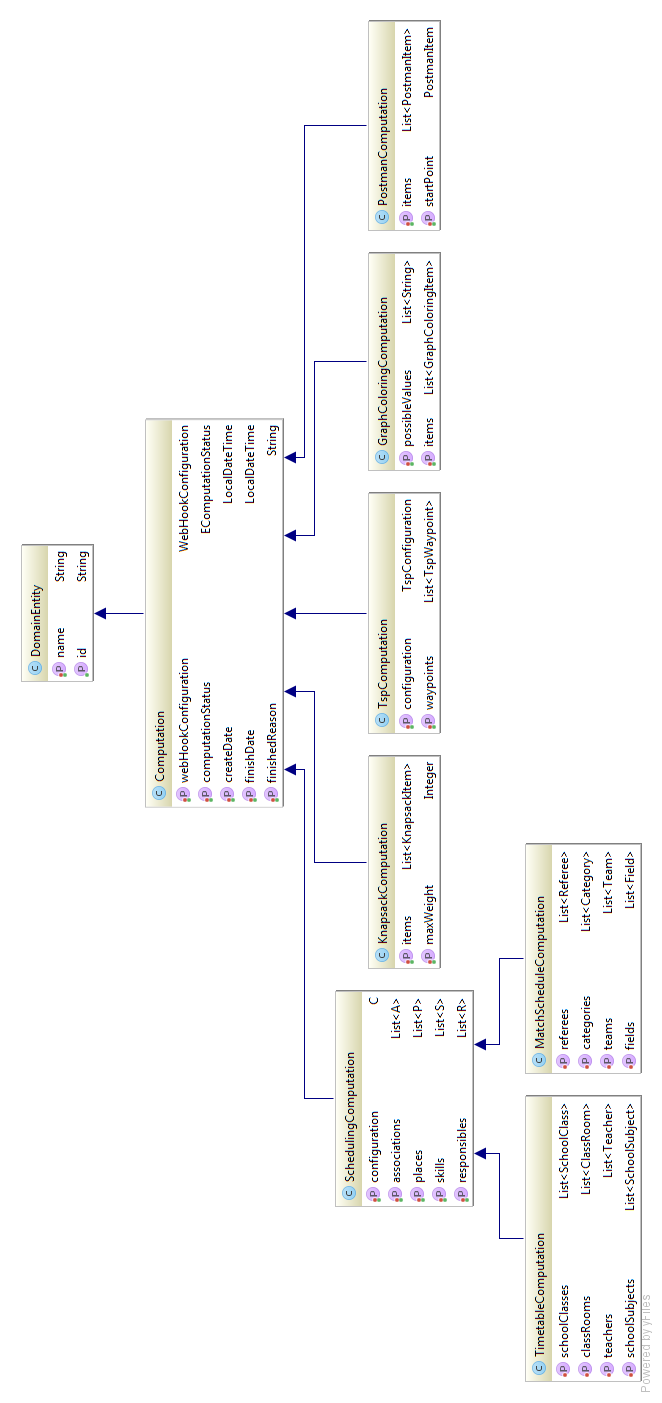
\includegraphics[scale=0.49]{images/computations_diagramm.png}
\caption[Klassendiagramm der verschiedenen Problemklassen]{Klassendiagramm der verschiedenen Problemklassen \selfmade{}}
\label{fig:problems_diagramm}
\end{figure}

\begin{figure}[h]
\centering
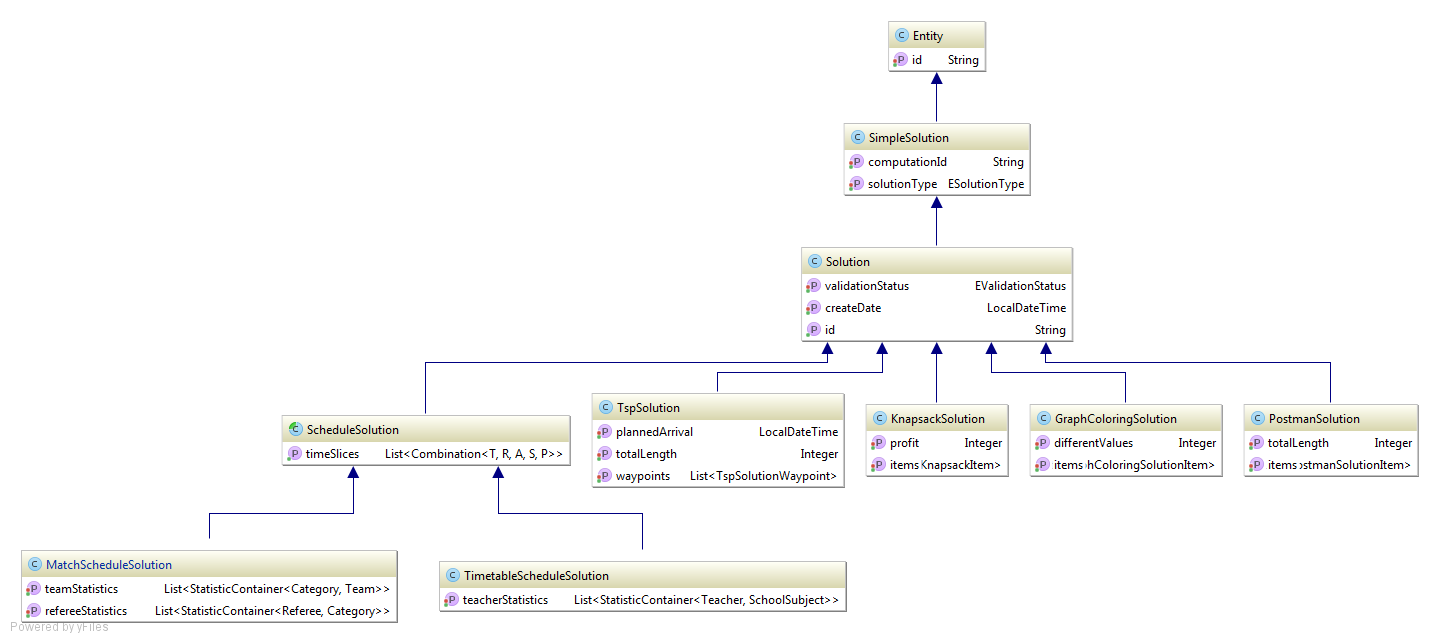
\includegraphics[scale=0.45]{images/solutions_diagramm.png}
\caption[Klassendiagramm der verschiedenen Resultatklassen]{Klassendiagramm der verschiedenen Resultatklassen \selfmade{}}
\label{fig:solutions_diagramm}
\end{figure}

\end{landscape}
 
%%%%%%%%%%%%%%%%%%%%%%%%%%%%%%%%%%%%%%%%%%%%%%%%%%%%%%%%%%%%%%%%%
%
% Project     : Bachelorarbeit
% Title       : Machbarkeitsanalyse für eine ressourcenorientierte Schnittstelle zur Verarbeitung grundlegender Probleme der Informatik
% File        : umsetzung.tex Rev. 01
% Date        : 01.03.2015
% Author      : Raffael Santschi
%
%%%%%%%%%%%%%%%%%%%%%%%%%%%%%%%%%%%%%%%%%%%%%%%%%%%%%%%%%%%%%%%%%

\chapter{Umsetzung des Prototyps \resultAssignment{[R5]}}\label{chap.umsetzung}
In diesem Kapitel wird kurz auf die Erkenntnisse aus dem \glslink{vertikaler_durchstich}{vertikalen Durchstich} eingegangen. Danach wird erklärt, wie die Umsetzung für die ausgewählten 
Problemtypen durchgeführt wurde. Zu guter Letzt wird noch die Entwicklungsumgebung für dieses Projekt beschrieben.

\section{Erster Durchstich}\label{entwicklungsumgebung}
Zum Start der Umsetzung wurde ein erster \gls{vertikaler_durchstich} anhand des Rucksack-Problems gemacht, um zu sehen, ob sich das Konzept bewährt. Während der 
Implementation wurde bereits überlegt, wie die Logik möglichst generisch gehalten werden kann.

\begin{figure}[h]
\centering
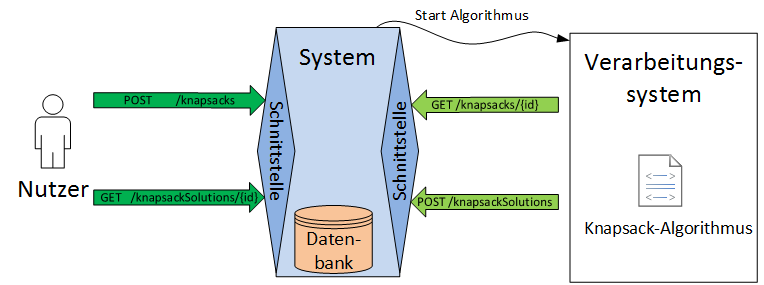
\includegraphics[scale=0.74]{images/visio/prototype_knapsack.png}
\caption[\Gls{vertikaler_durchstich} mit dem Rucksack-Problem]{Vertikaler Durchstich mit dem Rucksack-Problem \selfmade{}}
\label{fig:prototyp_knapsack}
\end{figure}

\subsection{Erkenntnisse nach dem ersten Durchstich}\label{learning_prototyp}
Die Kontaktschnittstelle nach aussen generisch zu halten, macht aus Gründen der Benutzerfreundlichkeit keinen Sinn. Für den Kunden ist es transparenter, wenn er eine Schnittstelle aufruft, 
welche zum Beispiel 'timetableComputations' heisst, statt einer generischen Schnittstelle namens 'computations'. Zudem ist es nicht möglich nur mithilfe der Daten herauszufinden, welches 
Problem gelöst werden möchte. Dazu würde es einen zusätzlichen Parameter benötigen. Weiter stellt es sich als schwierig heraus, mit Spring einen Endpunkt bereitzustellen, welcher 
verschiedene Ressourcentypen akzeptiert. Die Validierung der Eingabeparameter würde dadurch zusätzlich erschwert werden.

Das Konzept mit den beiden Translators bietet sehr viele Möglichkeiten und Flexibilität. Es entkoppelt die Nutzer-Schnittstelle komplett von der Schnittstelle für die Algorithmen. Um diese 
Flexibilität ausnutzen zu können, müssen jedoch oft verschiedene Entities für die Nutzer- und Algorithmus-Sicht erstellt werden.

In der Business Logik kann vieles generisch gehalten werden. Die Repositories, Services und die Interfaces können generisch programmiert werden und bleiben für alle Probleme gleich. Beim 
Controller kann die Logik in einer abstrakten Klasse definiert werden. Somit müssen nur noch die Namen der Schnittstellen in der spezifischen Implementation definiert werden. Es hat sich 
gezeigt, dass sich das Konzept bewährt und die weiteren Probleme dementsprechend gelöst werden konnten.

\subsection{Anpassung des Konzepts nach dem ersten Durchstich}\label{doings_prototyp}
Das Konzept wurde nach dem ersten \glslink{vertikaler_durchstich}{Durchstich} dahingegen geändert, dass die Schnittstellen auf der Nutzer-Seite umbenannt wurden und die 
Algorithmus-Seite einen anderen Namespace erhielt. Weiter verschwand die separate Schnittstelle für das Abfragen des Resultats, die Funktionalität wurde stattdessen in die Status-Abfrage 
integriert.

\section{Implementierung der Schnittstelle}\label{impl_interface}
In diesem Abschnitt wird über die Implementation der Schnittstelle im Allgemeinen geschrieben. Wie bereits erwähnt ist der Ablauf bei jedem Problem gleich, dementsprechend verhält sich die 
Schnittstelle im Allgemeinen gleich.

\subsection{Statusabfrage}
Damit der Nutzer möglichst wenig Schnittstellen ansprechen muss, erhält er bei einer Statusabfrage zugleich die vorhandenen Resultate. Der Nutzer erhält nur Resultate mit dem Status 'FINAL'. 
Resultate mit dem Status 'PARTIAL' werden zwar beim Status und der Zeit des zuletzt empfangenen Resultats berücksichtigt, aber nicht herausgegeben. Der Status besitzt neben den 
Resultaten eine ID und den Namen, weiter werden Startzeit, Endzeit und die Zeit des zuletzt empfangenen Resultats angegeben. Falls eine Berechnung beendet ist, wird eine 
Begründung der Beendigung angezeigt. Dies kann zum Beispiel ein aufgetretener Fehler während des Starts oder der Berechnung sein oder eine Bestätigung der erfolgreichen Berechnung.

\begin{lstlisting}[language=JSON, caption=Aufbau einer Antwort auf eine Statusabfrage, label=lst:status_response]  
{
  "id'': "<Berechnung ID>",
  "name": "<Berechnungsname>",
  "computationStatus": "<Status der Berechnung>",
  "createDate": <Erstelldatum>,
  "finishDate": <Enddatum>,
  "finishedReason": "<Begruendung der Beendigung>",
  "lastResultReceived": <Datum des zuletzt empfangenen Resultats>,
  "solutions": <Resultate>
}
\end{lstlisting}

\subsection{WebHook Möglichkeit}
Die Berechnungen können je nach Komplexität sehr lange dauern. Der Nutzer müsste immer wieder den Status abfragen, um zu sehen, ob ein Resultat vorhanden ist. \glspl{webhook} 
bieten Abhilfe für dieses Problem. Das Verfahren ist nicht standardisiert, es ist aber sehr simpel und hilfreich. Beim Start einer Berechnung kann eine URL mitgegeben werden, zu welcher 
bei jeder Statusänderung ein POST-Request gesendet wird. Um diese Schnittstelle möglichst generisch zu halten, wurde eine Möglichkeit geschaffen, eine beliebige Payload für den 
POST-Request anzugeben. Die Nachricht der Statusänderung kann nach belieben mit dem Platzhalter '\_\_MESSAGE\_\_' irgendwo in die Payload eingebunden werden. Das Attribut 'message' 
wird in der Nachricht gesetzt, wenn der Platzhalter nirgends verwendet wird. Eine Konfiguration für die Chat-Applikation 'Slack' würde wie in \autoref{lst:webhook_configuration} 
aussehen. Die Nachrichten bei Statusänderungen sähen dann wie in \autoref{fig:slack_chat} aus.

\begin{lstlisting}[language=JSON, caption=Beispiel einer WebHook Konfiguration für Slack, label=lst:webhook_configuration]
  ...  
  "webHookConfiguration": {
    "url": "https://hooks.slack.com/services/T0000/B0000/XXX",
    "payload": {
        "text": "__MESSAGE__",
        "channel": "#simplatyser",
        "username": "simplatyser",
        "icon_emoji": ":squirrel:"
    }
  }
 ...
\end{lstlisting}

\begin{figure}[h]
\centering
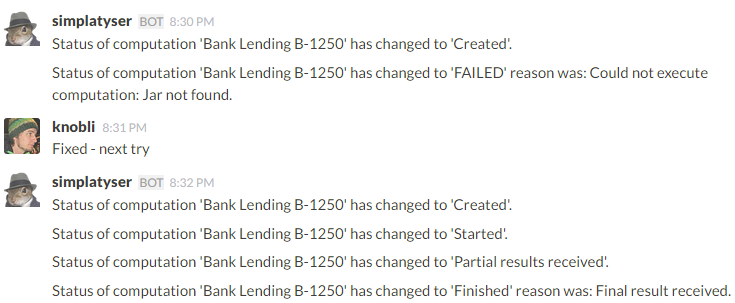
\includegraphics[scale=0.8]{images/slack_chat.png}
\caption[Nachrichten der Statusänderungen von Berechnungen]{Nachrichten der Statusänderungen von Berechnungen \selfmade{}}
\label{fig:slack_chat}
\end{figure}

\subsection{Technische Umsetzung und Probleme}
Das Fundament der Software war mit Spring Boot \cite{spring_boot} sehr schnell gebaut, die Anbindung an MongoDB wurde mit Spring Data \cite{spring_data} realisiert. Leider war 
oftmals die Dokumentation nicht ausreichend oder nur für die XML-Konfiguration von Spring ausgelegt. Weiter gab es fehlende Teile in Spring Data, welche gefunden werden mussten. 
So gibt es zum Beispiel zu diesem Zeitpunkt standardmässig keine Möglichkeit, ein 'LocalTime'-Objekt oder ein 'LocalDateTime'-Objekt von Java 8 zu persistieren. Dies führte zu einem 
Stackoverflow anstatt einer spezifischeren Exception, was wiederum die Suche nach dem Fehler erheblich erschwerte. Um diese Probleme zu beheben, musste ein eigener Converter 
geschrieben und dieser bei der MongoDB-Konfiguration angegeben werden.

Bei der Business Logik wurde geschaut, dass vieles mit \gls{generics} gelöst werden konnte. Vor allem bei den Services konnte viel Code für alle Probleme verwendet werden. Auch 
bei den beiden Scheduling-Problemen konnte viel Code-Duplizierung vermieden werden. Zusätzlich wurden häufig verwendete Funktionen, wie das Abbilden auf die Input-Objekte, in 
Helfer-Klassen ausgelagert, damit sie nur ein Mal implementiert werden mussten.

\section{Implementierung der Probleme}\label{impl_problems}
In diesem Unterkapitel wird für jedes Problem kurz erklärt, was beim Prototyp implementiert wurde, um die Möglichkeiten des Konzepts aufzuzeigen. Eine ausführliche 
Schnittstellen-Dokumentation ist in \autoref{api_doc} zu finden. Zusätzlich wurde noch eine elektronische Dokumentation der Schnittstelle mit Hilfe von Swagger UI erstellt. Diese stellt die 
angebotenen Schnittstellen, die Eingabeparameter und die Resultat sehr übersichtlich dar.

\begin{figure}[h]
\centering
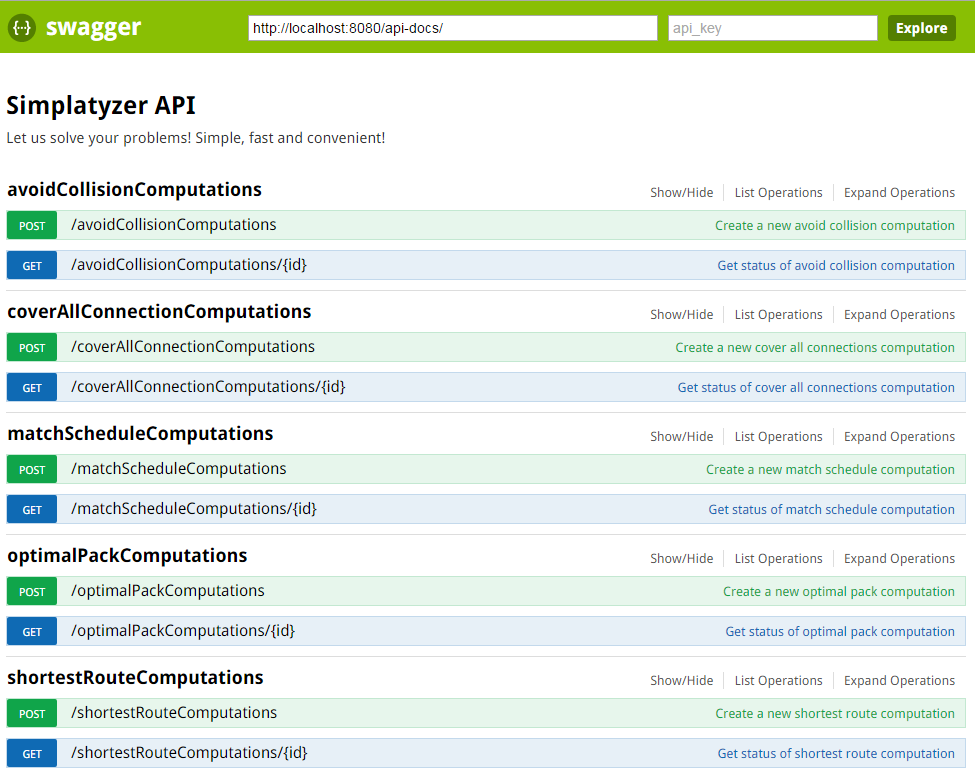
\includegraphics[scale=0.5]{images/swagger_api.png}
\caption[Nutzer-Schnittstellenbeschreibung von Swagger]{Nutzer-Schnittstellenbeschreibung von Swagger \selfmade{}}
\label{fig:swagger}
\end{figure}

\FloatBarrier

Beim Evaluieren des Stundenplan-Problems wurde bemerkt, dass es sehr viele verschiedene Planungsprobleme gibt. Deshalb wurde ein zusätzliches Planungsproblem gewählt, 
um zu schauen, wie sich die Schnittstelle bei sehr ähnlichen Problemen verhält.

%%%%%%%%%%%%%%%%%%%%%%%%%%%%%%%
%
%
%		Rucksack
%
%
%%%%%%%%%%%%%%%%%%%%%%%%%%%%%%%

\subsection{Rucksack}
Das Rucksack-Problem ist aus Sicht der Schnittstelle ein relativ einfaches Problem. Um die Benutzerfreundlichkeit zu verbessern, kann der Nutzer bei den Elementen eine Anzahl definieren und 
muss sie nicht doppelt angeben. Der Algorithmus hingegen bekommt eine Liste mit allen Elementen, es gibt nur noch einzelne Elemente und der Name wird nicht weitergegeben, da er vom 
Algorithmus nicht benötigt wird. Der Algorithmus liefert als Resultat eine Liste von booleschen Werten zurück, diese müssen zuerst wieder auf die ursprünglichen Elemente abgebildet werden. Bei 
der Validierung wird überprüft, ob die Gewichtsschranke nicht überschritten wurde und ob ein Element nicht zu oft verwendet wurde. Letzteres ist zwar beim getesteten Algorithmus nicht 
möglich, könnte jedoch bei einer anderen Implementation der Fall sein. Der Benutzer erhält als Resultat eine Liste mit allen Objekten, welche verwendet wurden. Wenn ein Objekt mehrmals 
verwendet wurde, wird die entsprechende Anzahl angegeben.

\begin{figure}[h]
\centering
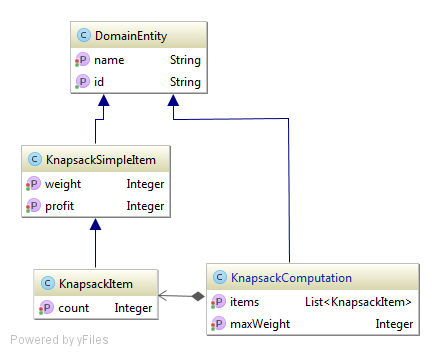
\includegraphics[scale=0.5]{images/probleme/knapsack.png}
\caption[Eingabeparameter für eine Rucksack-Berechnung]{Eingabeparameter für eine Rucksack-Berechnung \selfmade{}}
\label{fig:knapsack_input}
\end{figure}

\FloatBarrier

%%%%%%%%%%%%%%%%%%%%%%%%%%%%%%%
%
%
%		Knotenfärbung
%
%
%%%%%%%%%%%%%%%%%%%%%%%%%%%%%%%

\subsection{Knotenfärbung}
Bei der Knotenfärbung geht es darum, Kollisionen zu vermeiden. Dies wurde für den Nutzer möglichst transparent umgesetzt. Der Nutzer kann mögliche Werte (z.B. Farben oder 
Frequenzen) angeben, welche die Elemente zugeteilt bekommen sollen. Der Algorithmus erhält eine Liste mit allen Elementen und ihren Nachbarn. Die Namen der Elemente und die möglichen 
Werte werden nicht weitergegeben. Es wird davon ausgegangen, dass der Algorithmus eine Liste von Elementen mit den zugewiesenen Werten zurückgibt. Beim Übersetzen werden, falls 
vorhanden, die Werte vom Algorithmus mit den möglichen Werten aus der Benutzereingabe ausgetauscht. Bei der Validierung wird überprüft, dass kein Element den gleichen Wert wie einer 
seiner Nachbarn hat. Als Resultat erhält der Benutzer eine Liste mit allen Elementen und ihren zugewiesenen Werten.

\begin{figure}[h]
\centering
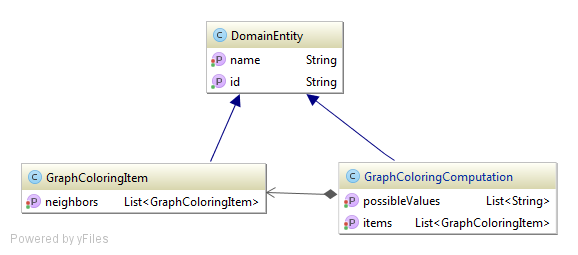
\includegraphics[scale=0.5]{images/probleme/graphcoloring.png}
\caption[Eingabeparameter für eine Knotenfärbung-Berechnung]{Eingabeparameter für eine Knotenfärbung-Berechnung \selfmade{}}
\label{fig:graphcoloring_input}
\end{figure}

%%%%%%%%%%%%%%%%%%%%%%%%%%%%%%%
%
%
%		Problem des Handlungsreisenden
%
%
%%%%%%%%%%%%%%%%%%%%%%%%%%%%%%%

\subsection{Problem des Handlungsreisenden}
Der Service bietet nicht nur die kürzeste Route für eine Liste von Wegpunkten an, es ist auch möglich, für jeden Wegpunkt eine gewünschte Ankunftszeit und Aufenthaltszeit anzugeben. Der 
Algorithmus erhält vom System eine Liste mit allen Wegpunkten, bei diesem Schritt wird nichts übersetzt. Es wäre jedoch theoretisch möglich, dass die Schnittstelle die Daten bereits für den 
Algorithmus aufbereitet, zum Beispiel indem sie die Distanzen zwischen den Wegpunkten berechnet. Es wird davon ausgegangen, dass der Algorithmus eine Liste der Wegpunkte in der 
berechneten Reihenfolge zurückgibt. Beim Übersetzen werden die geplanten Ankunftszeiten berechnet, welche dann während der Validierung mittels der maximal angegebenen Abweichung 
überprüft werden. Der Benutzer erhält als Resultat eine Liste von Wegpunkten mit gewünschter und geplanter Ankunftszeit in der berechneten Reihenfolge.

\begin{figure}[h]
\centering
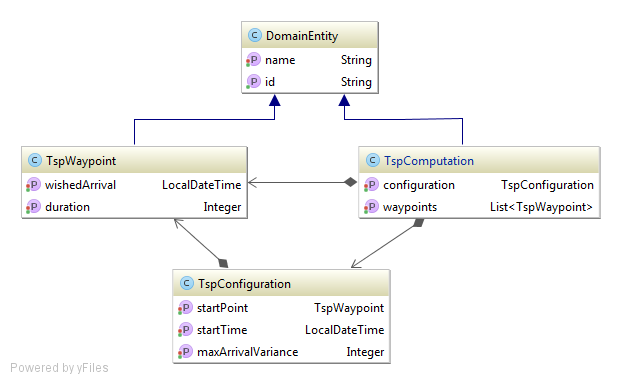
\includegraphics[scale=0.5]{images/probleme/tsp.png}
\caption[Eingabeparameter für eine Routen-Berechnung]{Eingabeparameter für eine Routen-Berechnung \selfmade{}}
\label{fig:tsp_input}
\end{figure}

%%%%%%%%%%%%%%%%%%%%%%%%%%%%%%%
%
%
%		Briefträgerproblem
%
%
%%%%%%%%%%%%%%%%%%%%%%%%%%%%%%%

\subsection{Briefträgerproblem}
Das Briefträgerproblem berechnet eine Route, welche alle bekannten Wege eines Graphen abfährt. Der Nutzer kann eine Liste von Wegpunkten mit den bekannten Verknüpfungen zu anderen 
Wegpunkten und ihrer Distanz angeben. Der Algorithmus erhält vom System eine Liste mit allen Wegpunkten, die Namen der Wegpunkte werden nicht weitergegeben. Es wird davon ausgegangen, 
dass der Algorithmus eine Liste der Wegpunkte in der berechneten Reihenfolge zurückgibt. Beim Übersetzen werden die Wegpunkte wieder auf die Eingabewerte abgebildet und die komplette 
Länge der Route berechnet. Die Validierung überprüft, ob der Weg möglich ist und ob jede Verbindung mindestens ein Mal benutzt wurde. Der Benutzer erhält als Resultat eine Liste mit der berechneten 
Reihenfolge der Wegpunkte und die totale Länge der Strecke.

\begin{figure}[h]
\centering
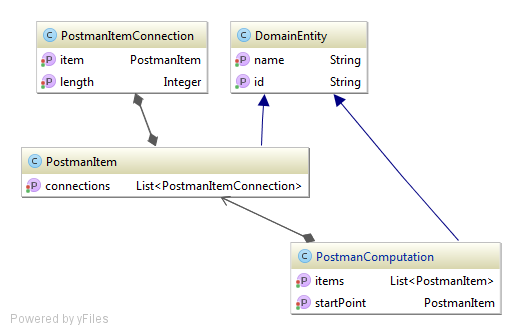
\includegraphics[scale=0.5]{images/probleme/postman.png}
\caption[Eingabeparameter für eine Briefträger-Routen-Berechnung]{Eingabeparameter für eine Briefträger-Routen-Berechnung \selfmade{}}
\label{fig:postman_input}
\end{figure}

\FloatBarrier
%%%%%%%%%%%%%%%%%%%%%%%%%%%%%%%
%
%
%		Stundenplan Erstellung
%
%
%%%%%%%%%%%%%%%%%%%%%%%%%%%%%%%

\subsection{Stundenplan Erstellung}
Das Erstellen eines Stundenplans ist ein Planungsproblem, welches sehr viele Möglichkeiten und Einschränkungen besitzt und somit sehr komplex ist. In dieser Implementation sind bei weitem 
nicht alle Spezialitäten abgedeckt. Es wurde geschaut, dass bereits einige Einschränkungen, wie zum Beispiel freie Tage von Lehrern und blockierte Schulzimmer, miteinbezogen werden. 
Der Nutzer gibt eine Liste von Klassen, Lehrern, Schulzimmern und Schulfächern an. Die Klassen haben eine bestimmte Grösse und definieren auch, welche Fächer sie besuchen müssen. Die 
Lehrer haben eine Liste mit Schulfächern, welche sie unterrichten können, eine List mit zugehörigen Klassen und eine Definition ihrer freien Tage. Die Klassenzimmer besitzen eine Liste mit 
möglichen Schulfächern und eine Sperrliste, in welcher definiert ist, wann der Raum nicht verfügbar ist. Die Schulfächer können definieren, ob sie eine Raum brauchen, welcher explizit dafür 
bestimmt ist, zum Beispiel Sport in der Turnhalle. Neben den zu verplanenden Elementen gibt es Randbedingungen wie die Pausenzeiten, die Lektionsdauer und die Definition, 
wann unterrichtet werden soll. Der Algorithmus erhält eine Liste mit allen Klassen, Lehrern, Schulzimmern und Schulfächern. Die Rahmenbedingungen werden in Zeitfenster umgewandelt, 
welche vom Algorithmus verplant werden können. Zusätzlich werden die Elemente generischer benannt, damit der Algorithmus nicht verschiedene Konfigurationen für verschiedene 
Planungsprobleme besitzen muss. In \autoref{lst:cat_input_timetableScheduling} ist ein Beispiel für eine Eingabe der Rahmenbedingungen gezeigt, welche durch den Translator in die Zahl 36 
umgewandelt wird. Die Zahl wird aus der Lektionsdauer, den Pausen und den einzelnen Zeitfenstern pro Tag berechnet, die \autoref{table:timeslice_calc} stellt dies visuell dar.

\begin{lstlisting}[language=JSON, caption=Ausschnitt einer Eingabe für das Stundenplanproblem für die Rahmenbedingungen, label=lst:cat_input_timetableScheduling]  
{
  ...
  "configuration": {
    "breakTimeSliceSize": [5, 20, 5, 90, 5, 20, 5],
    "dayTimeSlots": [
      {
        "monday": {"defaultTimes": true},
        "tuesday": {"defaultTimes": true},
        "wednesday": {"from": [8, 20, 0], "to": [12,0,0]},
        "thursday": {"defaultTimes": true},
        "friday": {"defaultTimes": true}
      }
    ],
    "lessonDuration": 45
  }
}
\end{lstlisting}

\begin{table}[ht]
\centering
  \begin{tabular}{ l | c | c | c | c | c }
	\hline
	\rowcolor{gray}
	\textbf{Uhrzeit} 	& \textbf{Mo}	& \textbf{Di} 	& \textbf{Mi}	&  \textbf{Do}	&  \textbf{Fr}\\ \hline
	0820-0905		& 1			& 9			& 17			& 21			& 29		\\ \hline
	0910-0955		& 2			& 10			& 18			& 22			& 30		\\ \hline
	1015-1100		& 3			& 11			& 19			& 23			& 31		\\ \hline
	1105-1150		& 4			& 12			& 20			& 24			& 32		\\ \hline \hline
	1320-1405		& 5			& 13			& -			& 25			& 33		\\ \hline
	1410-1455		& 6			& 14			& -			& 26			& 34		\\ \hline
	1515-1600		& 7			& 15			& -			& 27			& 35		\\ \hline
	1605-1650		& 8			& 16			& -			& 28			& 36		\\ \hline
  \end{tabular}
   \caption{Visuelle Darstellung der Zeitfenster-Berechnung}\label{table:timeslice_calc}
\end{table}

\begin{figure}[h]
\centering
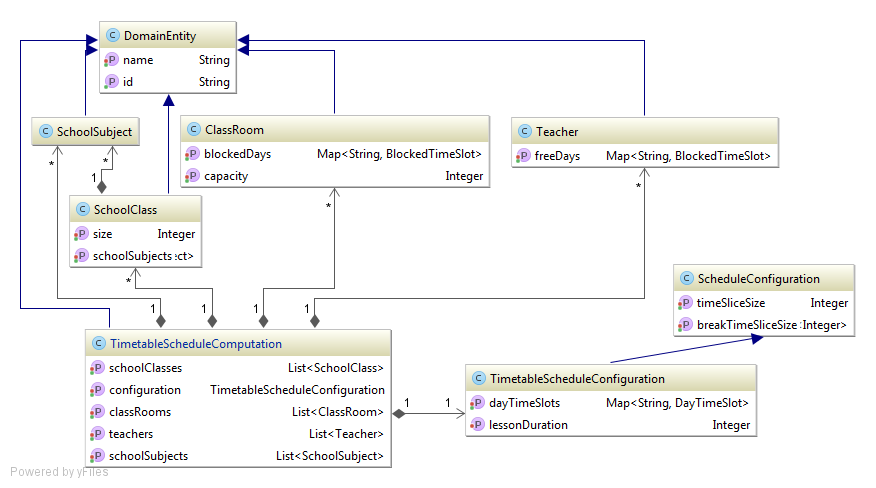
\includegraphics[scale=0.5]{images/probleme/timetableSchedule.png}
\caption[Eingabeparameter für eine Stundenplan-Berechnung]{Eingabeparameter für eine Stundenplan-Berechnung \selfmade{}}
\label{fig:timetableSchedule_input}
\end{figure}

\FloatBarrier

Es wird davon ausgegangen, dass der Algorithmus eine Liste von Planungskombinationen zurückgibt. Eine Kombination besteht aus einer Zeitfensternummer, einem Lehrer, einer Klasse, 
einem Schulfach und einem Klassenzimmer. Beim Übersetzen werden die IDs auf die ursprünglichen Elemente abgebildet, die Zeitfensternummern wieder werden in Uhrzeiten umgewandelt. 
Zusätzlich wird eine Statistik für die Lehrer geführt. Bei der Validierung wird geschaut, ob ein Element zu einer Zeit mehrfach verplant ist, ob der Lehrer die nötigen Fähigkeiten hat und ob ein 
Klassenzimmer für das Fach ausgelegt ist. Das umgewandelte Resultat enthält eine Liste mit den berechneten Kombination, sortiert nach Wochentag und Uhrzeit. Die Lehrerstatistik zeigt, wie 
oft ein Lehrer ein bestimmtes Fach und wie viele Stunden er insgesamt unterrichtet.

%%%%%%%%%%%%%%%%%%%%%%%%%%%%%%%
%
%
%		Spielplan Erstellung
%
%
%%%%%%%%%%%%%%%%%%%%%%%%%%%%%%%

\subsection{Spielplan Erstellung}
Eine weitere Ausprägung des Planungsproblems ist das Erstellen eines Spielplans. Der Nutzer gibt eine Liste von Teams, Schiedsrichtern, Spielfeldern und Kategorien an. Die Teams haben eine 
bestimmte Kategorie. Die Schiedsrichter haben eine Liste mit Kategorien, welche sie leiten können, und eine Liste von Teams, zu welchen sie gehören. Die Spielfelder besitzen eine Liste mit 
möglichen Kategorien. Neben den zu verplanenden Elementen gibt es Randbedingungen wie die Spieldauer, die Startzeit und die Pausenzeiten. Der Algorithmus erhält eine 
Liste mit allen Teams, Schiedsrichtern, Spielfeldern und Kategorien. Zusätzlich werden die Elemente generischer benannt, damit der Algorithmus nicht verschiedene Konfigurationen für 
verschiedene Planungsprobleme besitzen muss.

\begin{figure}[h]
\centering
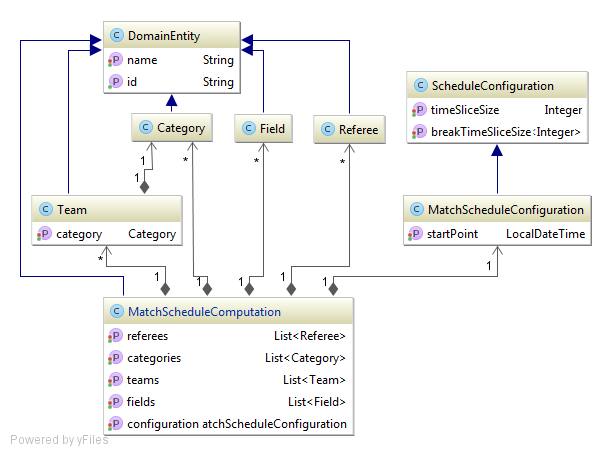
\includegraphics[scale=0.5]{images/probleme/matchSchedule.png}
\caption[Eingabeparameter für eine Spielplan-Berechnung]{Eingabeparameter für eine Spielplan-Berechnung \selfmade{}}
\label{fig:matchschedule_input}
\end{figure}

Es wird davon ausgegangen, dass der Algorithmus eine Liste von Planungskombinationen zurückgibt. Eine Kombination besteht aus einer Zeitfensternummer, einem Schiedsrichter, 
einer Kombination von zwei Teams und einem Spielfeld. Beim Übersetzen werden die IDs auf die ursprünglichen Elemente abgebildet, die Zeitfensternummern werden wieder in Uhrzeiten 
umgewandelt. Zusätzlich wird eine Statistik über die Einsätze der Schiedsrichter und der Teams geführt. Bei der Validierung wird geschaut, ob ein Element zu einer 
bestimmten Zeit mehrfach verplant ist, ob die Schiedsrichter die nötigen Fähigkeiten haben und ob ein Spielfeld für die Kategorie ausgelegt ist. Der Benutzer erhält als Resultat eine Liste 
mit den berechneten Kombination, sortiert nach Uhrzeit. Die Schiedsrichterstatistik zeigt, wie oft ein Schiedsrichter eine bestimmte Kategorie pfeift und für wie viele Spiele er insgesamt 
verantwortlich ist. Die Teamstatistik zeigt, wie viele Spiele eine Kategorie insgesamt hat und wie viele Spiele ein Team bestreitet. In \autoref{lst:cat_result_matchScheduling} wird ein 
Ausschnitt der Schiedsrichterstatistik dargestellt.

\begin{lstlisting}[language=JSON, caption=Ausschnitt eines Resultats einer Spielplan Erstellung, label=lst:cat_result_matchScheduling]  
{
  ...
  name: "Sabine Pfister"
  statisticMap: {
    Knaben: 1
    Damen Kat A: 3
    Damen Kat B: 2
    _TOTAL: 6
  }
  ...
}
\end{lstlisting}

\subsection{Übersicht der Schnittstellen}
Für den Nutzer wurde ein problem-agnostischer Name für die Schnittstelle gewählt. Die Namen unterscheiden sich somit zum Teil zwischen Nutzer- und Algorithmus-Sicht. Damit die 
Verknüpfung der beiden Schnittstellen nicht verloren geht, und um eine Übersicht über alle angebotenen Schnittstellen zu haben, wurden sie in der \autoref{table:overview_api_interfaces} 
zusammengetragen. Die Endpunkte für die Algorithmen sind unter dem Namespace '/algorithm', damit diese beiden sauber voneinander getrennt sind.

\begin{table}[ht]
\centering
  \begin{tabular}{ l | l }
	\hline
	\rowcolor{gray}
	\textbf{Nutzer}							& \textbf{Algorithmus}					\\ \hline
	/									& /algorithm/							\\ \hline
	\multicolumn{2}{|c|}{\textbf{Allgemein / Beschreibung}}\\ \hline
	 Berechnung starten				& Berechnungsinformationen abholen			\\ \hline
	Status bzw. Lösung	abholen & Lösung bekannt geben	\\ \hline
	\multicolumn{2}{|c|}{\textbf{Rucksack}}\\ \hline
	 POST /optimalPackComputations					& GET /knapsackComputations/\{ID\}			\\ \hline
	GET /optimalPackComputations/\{ID\}	& POST /knapsackComputations/\{ID\}/solutions	\\ \hline
	\multicolumn{2}{|c|}{\textbf{Knotenfärbung}}\\ \hline
	POST /avoidCollisionComputations				& GET /graphColoringComputations/\{ID\}		\\ \hline
	GET /avoidCollisionComputations/\{ID\}		& POST /graphColoringComputations/\{ID\}/solutions	\\ \hline
	\multicolumn{2}{|c|}{\textbf{Problem des Handlungsreisenden}}\\ \hline
	POST /shortestRouteComputations				& GET /tspComputations/\{ID\}				\\ \hline
	GET /shortestRouteComputations/\{ID\}		& POST /tspComputations/\{ID\}/solutions		\\ \hline
	\multicolumn{2}{|c|}{\textbf{Briefträgerproblem}}\\ \hline
	POST /coverAllConnectionComputations				& GET /postmanComputations/\{ID\}			\\ \hline
	GET /coverAllConnectionComputations/\{ID\} 	& POST /postmanComputations/\{ID\}/solutions	\\ \hline
	\multicolumn{2}{|c|}{\textbf{Stundenplan Erstellung}}\\ \hline
	POST /timetableComputations				& GET /timetableComputations/\{ID\}			\\ \hline
	GET /timetableComputations/\{ID\}	& POST /timetableComputations/\{ID\}/solutions	\\ \hline
	\multicolumn{2}{|c|}{\textbf{Spielplan Erstellung}}\\ \hline
	POST /matchesScheduleComputations				& GET /matchesScheduleComputations/\{ID\}			\\ \hline
	GET /matchesScheduleComputations/\{ID\}	& POST/matchesScheduleComputations/\{ID\}/solutions	\\ \hline
  \end{tabular}
   \caption{Übersicht der angebotenen Schnittstellen}\label{table:overview_api_interfaces}
\end{table}

\FloatBarrier

\subsection{Erstellung eines neuen Problems}
Das Ziel dieser Arbeit war die Erstellung einer Schnittstelle, welche einfach zu erweitern ist. Dieser Abschnitt soll zeigen, wie dies erreicht wurde und wie sie erweitert werden kann. Das 
Software-Projekt ist in Packages gegliedert. Auf der ersten Ebene befinden sich die generischen Klassen. Die spezifischen Implementierungen sind unter dem Package 'problem'  angesiedelt. 
Die Gliederung ist so gewählt, damit ein Problem nur an einem Ort im Projekt vorhanden ist und nicht an vielen verschiedenen Stellen gesucht werden muss. Es wäre auch möglich, 
die verschiedenen Problem-Implementationen in ein anderes Projekt auszulagern.

Um ein neues Problem in den Katalog aufzunehmen, muss ein neues Package mit dem Problemnamen erstellt werden. Darin sind weitere Packages zur besseren Übersicht definiert. Als 
erstes muss das Problem analysiert werden und dementsprechend die Entities für die Eingabe und das Resultat bereit gestellt werden.

Sind die Entities definiert, muss je ein Controller für den Algorithmus den Nutzer erstellt werden. Die Controller leiten von einer abstrakten Klasse ab und dienen lediglich zur Definition
der neuen Endpunkte. Die Dokumentation der Controller wird in die jeweiligen Klassen geschrieben, dies erweitert automatisch die elektronische Dokumentation von Swagger UI. 
Nun fehlen noch die beiden Translators für das Umwandeln der Nutzer-Sicht in die Algorithmus-Sicht, der Validator für das Problem und der Solver, welcher den Algorithmus 
startet. Alles andere ist generischer Code, welcher nur noch mit den jeweiligen Entity-Typen spezifiziert werden muss.

Zu guter Letzt wird noch ein Beispiel für eine Eingabe aus Nutzer-Sicht und ein Resultat aus Algorithmus-Sicht in JSON unter den Ressourcen abgelegt. Diese Beispiele können für Tests 
verwendet werden.

\newpage

\section{Entwicklungsumgebung}\label{entwicklungsumgebung}
Ein Softwareprojekt benötigt immer eine gewisse Entwicklungsumgebung. Bei der Entwicklung mit Spring Boot sind die Anforderungen minimal, da Spring Boot bereits einen eigenen Webserver 
mitbringt.

\subsection{IDE - Integrated Development Environment}
Als \gls{ide} wurde IntelliJ \cite{intellij} verwendet, IntelliJ bietet gute Refactoring-Methoden und Unterstützung beim Programmieren von Java-Code an. Die \gls{ide} 
bietet auch die Möglichkeit, Klassen-Diagramme zu erstellen und hat ein \gls{vim}-Plugin. Mit diesem Plugin können \gls{vim}-Befehle benutzt werden, was die 
Geschwindigkeit beim Programmieren enorm erhöht.

\begin{figure}[h]
\centering
\includegraphics[scale=0.7]{images/IntelliJ.png}
\caption[Darstellung der Package-Struktur in IntelliJ]{Darstellung der Package-Struktur in IntelliJ \selfmade{}}
\label{fig:IntelliJ}
\end{figure}

\newpage

\subsection{Versionierung}
Für die Versionierung der Software wurde git \cite{git} verwendet. Das Remote Repository wurde auf Github \cite{github_simplatyzer} erstellt. Es wurde darauf geachtet, dass 
der Code oft ins Repository geladen wurde, damit ein Backup existiert. Die Dokumentation wurde in Dropbox \cite{dropbox} gespeichert, damit auf verschiedenen Computern darauf 
zugegriffen werden konnte und immer ein Backup vorhanden war. Zu Korrekturzwecken wurde die Arbeit ebenfalls auf Github hochgeladen und die Änderungsvorschläge wurden mit Latexdiff 
\cite{latexdiff} verglichen.

\begin{figure}[h]
\centering
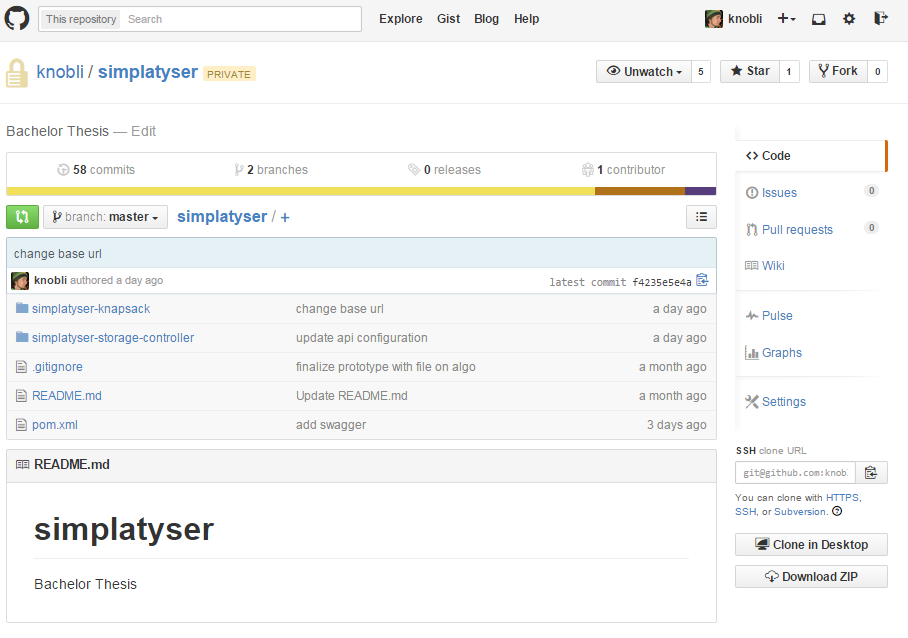
\includegraphics[scale=0.6]{images/github.png}
\caption[Github Repository des Simplatyser Projekts]{Github Repository des Simplatyser Projekts \selfmade{}}
\label{fig:github_repo}
\end{figure}

\FloatBarrier
\newpage

\subsection{Testen - Analysieren}
Über die Chrome App 'Advanced REST client' \cite{advanced_rest_client} (siehe Abbildung \ref{fig:advanced_rest_client})  wurde die Schnittstelle manuell getestet. Für die Regression-Tests 
wurde JUnit \cite{junit} und Mockito \cite{mockito} verwendet. Die statische Code Analyse wurde mit \gls{sonar} \cite{sonar} durchgeführt.

\begin{figure}[h]
\centering
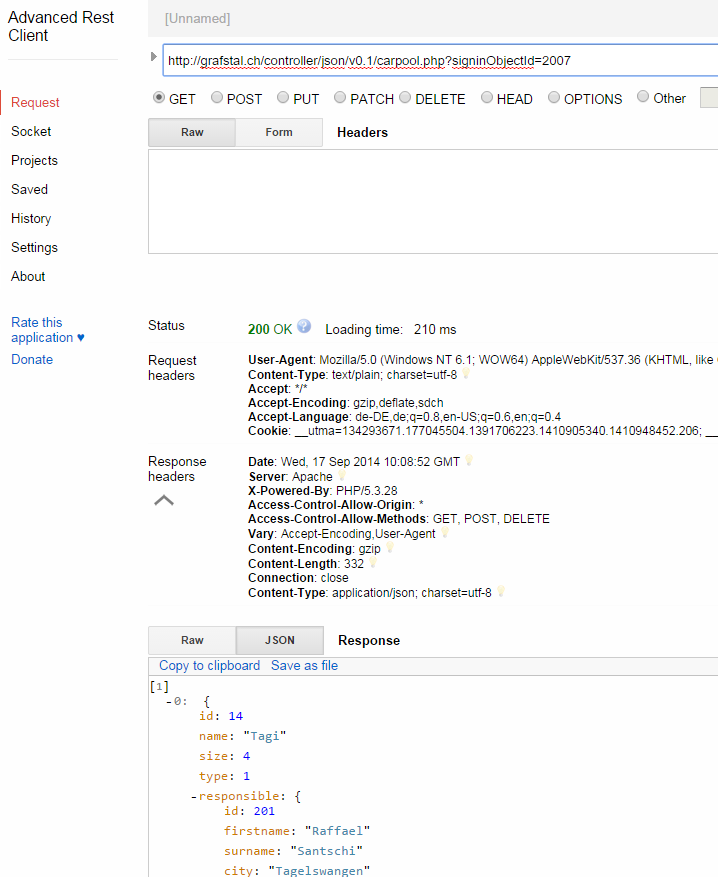
\includegraphics[scale=0.65]{images/advanced_rest_client.png}
\caption[Advanced REST client]{Advanced REST client \selfmade{}}
\label{fig:advanced_rest_client}
\end{figure}
%%%%%%%%%%%%%%%%%%%%%%%%%%%%%%%%%%%%%%%%%%%%%%%%%%%%%%%%%%%%%%%%%
%
% Project     : Bachelorarbeit
% Title       : Machbarkeitsanalyse für eine ressourcenorientierte Schnittstelle zur Verarbeitung grundlegender Probleme der Informatik
% File        : tests.tex Rev. 01
% Date        : 01.03.2015
% Author      : Raffael Santschi
%
%%%%%%%%%%%%%%%%%%%%%%%%%%%%%%%%%%%%%%%%%%%%%%%%%%%%%%%%%%%%%%%%%

\chapter{Tests \resultAssignment{[R6]}}\label{chap.tests} 
In diesem Kapitel wird auf das Testverfahren und die Tests für dieses Projekts eingegangen.

\section{Einführung}
In diesem Projekt wurden die sieben Grundsätze aus \cite{test_soft_book} als Leitlinie zum Testen verwendet:
\begin{enumerate}
\item \textbf{Testen zeigt die Anwesenheit von Fehlern}: Die Testabdeckung wurde mit Hilfe von IntelliJ ermittelt und anhand der Anforderungen überprüft.
\item \textbf{Vollständiges Testen ist nicht möglich}: Es wurde solange getestet bis alle Akzeptanzkriterien abgedeckt waren und die Testabdeckung gut genug war.
\item \textbf{Mit dem Testen frühzeitig beginnen}: Die Unit Tests für neue Funktionen wurden möglichst zeitnah oder zur gleichen Zeit geschrieben.
\item \textbf{Häufung von Fehlern}: Wenn Fehler in einer Komponente auftraten, dann wurde diese nach der Behebung nochmals intensiv getestet und zusätzliche Tests erfasst.
\item \textbf{Zunehmende Testresistenz (Pesticide paradox)}: Jede Änderungen am Code hatte auch eine Anpassung oder Erweiterung der Tests zur Folge.
\item \textbf{Testen ist abhängig vom Umfeld}: Der Prototyp ist nicht sicherheitskritisch, jedoch wurde Wert auf eine hohe Testabdeckung gelegt. Es wurden zusätzlich immer wieder 
	End-zu-End Tests mit den verschiedenen Problemen durchgeführt.
\item \textbf{Trugschluss: Keine Fehler bedeutet ein brauchbares System}: Die Schnittstelle wurde dem \gls{stakeholder} demonstriert und erklärt bevor das Projekt zu Ende war. So 
	konnten allfällige Missverständnise frühzeitig erkannt werden. Die hohe Testabdeckung trägt ebenfalls zur Aufdeckung von unbemerkten Fehlern bei.
\end{enumerate}

\section{Testing}
Komponententests und Integrationstests, bekannt aus \cite{test_soft_book}, wurden bei der Schnittstelle mit JUnit und Mockito durchgeführt. Bei den Integrationstests wurde eine 
Testdatenbank verwendet, welche bei jedem Testlauf neu initialisiert wird. Die Ausgangslage ist somit für jeden Durchlauf identisch. Für die Analyse der Testabdeckung wurde IntelliJ 
verwendet und die statische Code Analyse wurde mit \gls{sonar} ausgeführt. Neben den automatischen Tests wurden immer wieder manuelle Tests durchgeführt, um auch das Nutzererlebnis 
zu testen.

\section{Systemtest}
Als Abschluss des Projekts wurde ein Systemtest durchgeführt, für welcher ein Testprotokoll erstellt wurde. Das Protokoll zeigt dem Kunden die Testabfolge und das Ergebnis.

\subsection{Testprotokoll}
Das Testprotokoll basiert auf den Use Cases (siehe Abschnitt \ref{use_cases}) und den Anforderungen (Abschnitt \ref{anforderungen}). Akzeptanzkriterien mit UND- oder ODER-Verknüpfung 
wurden aufgesplittet, um sicher zu gehen, dass beide Bedingungen erfüllt sind.

%%\begin{longtable}{ l | p{7cm} | l | l }
\begin{longtable}{>{\raggedright}m{1cm}m{6cm}m{3.5cm}m{3cm}}

\caption[Testprotokoll]{\label{table:tests}Testprotokoll}\\ 
\toprule
\textbf{ID}&\textbf{Test}&\textbf{Herkunft}&\textbf{nicht / teilweise / erfüllt}\\ \midrule\addlinespace
\endfirsthead
\caption*{\textbf{Tabelle~\ref{table:tests} (Fortsetzung):} Testprotokoll}\\ \toprule
\textbf{ID}&\textbf{Test}&\textbf{Herkunft}&\textbf{nicht / teilweise / erfüllt}\\ \midrule\addlinespace
\endhead

\bottomrule\multicolumn{2}{>{\small\raggedleft\arraybackslash}r}{\slshape Fortsetzung auf der nächsten Seite}\\
\endfoot
\bottomrule
\endlastfoot	

	\addlinespace
	1	&	Der Nutzer kann eine Schnittstelle für die bereitgestellte Berechnungsfunktionen ansprechen.			
				&	\nameref{table:req_1} 	&	erfüllt\\ \addlinespace\hline \addlinespace
	2	&	Die Parameter sind persistent.			
				&	\nameref{table:req_3} 	&	erfüllt\\ \addlinespace\hline \addlinespace
	3a	&	Es gibt eine Fehlermeldung, falls bei der Speicherung etwas fehlschlägt			
				&	\nameref{table:req_3} 	&	erfüllt\\ \addlinespace\hline \addlinespace
	3b	&	oder die Eingabeparameter nicht gültig sind.			
				&	\nameref{table:req_3} 	&	erfüllt\\ \addlinespace\hline \addlinespace				
	4	&	Der Nutzer erhält nach dem Start einer Berechnung eine ID.
				&	\nameref{table:req_2} 	&	erfüllt\\ \addlinespace\hline \addlinespace
	5a	&	Der Befehl für den Start wird versendet		
				&	\nameref{table:req_4} 	&	erfüllt\\ \addlinespace\hline \addlinespace
	5b	&	und die ID dabei übergeben.		
				&	\nameref{table:req_4} 	&	erfüllt\\ \addlinespace\hline \addlinespace				
	6	&	Die Fehlermeldung bei einem Fehlversuch wird gespeichert.
				&	\nameref{table:req_4} 	&	erfüllt\\ \addlinespace\hline \addlinespace
	7	&	Das Verarbeitungssystem erhält die Eingabeparameter.
				&	\nameref{table:req_5} 	&	erfüllt\\ \addlinespace\hline \addlinespace
	8	&	Das Verarbeitungssystem erhält eine Fehlermeldung, falls keine Eingabeparameter vorhanden sind.
				&	\nameref{table:req_5} 	&	erfüllt\\ \addlinespace\hline \addlinespace
	9	&	Der Nutzer erhält einen Status seiner Berechnung.
				&	\nameref{table:req_6} 	&	erfüllt\\ \addlinespace\hline \addlinespace
	10	&	Der Nutzer wird über die Änderungen des Status auf dem eingetragen Dienst informiert.
				&	\nameref{table:req_7} 	&	erfüllt\\ \addlinespace\hline \addlinespace
	11	&	Das Verarbeitungssystem kann das Resultat abspeichern.
				&	\nameref{table:req_8} 	&	erfüllt\\ \addlinespace\hline \addlinespace
	12	&	Das Verarbeitungssystem erhält eine Fehlermeldung, falls das Speichern fehlgeschlagen ist.
				&	\nameref{table:req_8} 	&	erfüllt\\ \addlinespace\hline \addlinespace
	13	&	Der Nutzer erhält das Resultat der Berechnung.
				&	\nameref{table:req_9} 	&	erfüllt\\ \addlinespace\hline \addlinespace
	14	&	Der Nutzer erhält eine entsprechende Fehlermeldung, wenn beim Bereitstellen des Resultats ein Fehler aufgetreten ist.
				&	\nameref{table:req_9} 	&	erfüllt\\ \addlinespace\hline \addlinespace
	15	&	Das Interface kann verwendet werden, ohne dass das Verarbeitungssystem bekannt ist.
				&	\nameref{table:req_nf_1} 	&	erfüllt\\ \addlinespace\hline \addlinespace
	16	&	Unterschiedliche Ausprägungen eines Problems benutzen das gleiche API.
				&	\nameref{table:req_nf_2} 	&	teilweise erfüllt\\ \addlinespace\hline \addlinespace
	17	&	Unterschiedliche Probleme haben kein abweichendes Persistierungsschema.
				&	\nameref{table:req_nf_3} 	&	erfüllt\\ \addlinespace\hline \addlinespace
	18	&	Die Schnittstelle kann mit wenig Aufwand erweitert werden.
				&	\nameref{table:req_nf_4} 	&	erfüllt\\ \addlinespace\hline \addlinespace					

\end{longtable}
%%%%%%%%%%%%%%%%%%%%%%%%%%%%%%%%%%%%%%%%%%%%%%%%%%%%%%%%%%%%%%%%%
%
% Project     : Bachelorarbeit
% Title       : Machbarkeitsanalyse für eine ressourcenorientierte Schnittstelle zur Verarbeitung grundlegender Probleme der Informatik
% File        : fazit.tex Rev. 01
% Date        : 01.03.2015
% Author      : Raffael Santschi
%
%%%%%%%%%%%%%%%%%%%%%%%%%%%%%%%%%%%%%%%%%%%%%%%%%%%%%%%%%%%%%%%%%


\chapter{Schlussfolgerungen}\label{chap.Schlussfolgerungen}
In der Schlussfolgerung wird kurz auf die Verwendung des Produktes, das Fazit des Verfassers und den Ausblick eingegangen.

\section{Verwendung}\label{fazit_verwendung}
Während der Projektzeit konnte der Spielplan des Auffahrtsturniers des Turnvereins Grafstals validiert werden. Dieser Spielplan wird von Hand erstellt und immer wieder unterlaufen 
kleine Patzer, was bei einer Planung von etwa 110 Spielen und Schiedsrichtern, welche Coaches für bis zu drei Teams sind, nicht verwunderlich ist. Diese Aufgabe hat zum einen die Schnittstelle 
getestet, hat jedoch auch dem Verein geholfen, da auch dieses Jahr zwei kleine Fehler auftauchten. Der Turnverein hat sich bereits sehr für die vollautomatisierte Lösung interessiert.

\section{Fazit}\label{fazit}

Das Erstellen eines Konzept einer solchen Schnittstelle stellte sich als sehr spannend heraus. Die Recherche und die Analyse der Probleme mit hoher Laufzeitkomplexität war sehr fesselnd und es 
bestand die Gefahr sich darin zu verlieren. Das Gebiet der theoretischen Informatik ist extrem weitreichend und die Probleme können beliebig komplex werden. Es war schnell klar, dass es schwierig 
sein wird, eine generische Lösung für die Probleme zu finden. Das Konzept mit dem pre- und post-Aktionen ist eine elegante Lösung und bietet sehr viel Flexibilität. Der Ablauf einer Berechnung 
konnte generisch gehalten werden und somit ist die Machbarkeitsstudie als erfolgreich zu betrachten.

Die Auswahl der Probleme hat sich als facettenreich herausgestellt und das Auswahlverfahren hat sich bewährt. Es ist spannend, dass die beiden Probleme aus dem Bereich `Netzwerk Design' 
viele Ähnlichkeiten aufzeigen, jedoch mit komplett anderen Algorithmen gelöst werden. Die beiden Planungsprobleme sind sich sehr ähnlich und könnten ziemlich sicher mit einem generischen 
Algorithmus gelöst werden. Der grösste Unterschied liegt darin, dass bei einem Spielplan zwei Mannschaften gleichzeitig auf einem Platz sind und bei einem 
Stundenplan jeweils nur eine Klasse. Der Code der Schnittstelle konnte für die beiden Planungsprobleme auch viel generischer gehalten werden als für diejenigen aus dem Bereich 
`Netzwerk Design'.

Der Entscheid, eine dokumentorientierte Datenbank zu verwenden, war ideal. Die Flexibilität der Datenbank kam dem Projekt sehr zugute und es wurde keine Funktion vermisst. Spring Boot ist für 
einen Prototyp ideal, da es schon sehr viel mitbringt. Dies kann jedoch auch zu Problemen führen, da die Versionen von den Libraries nicht selber verwaltet werden können. 

Ich bin mit dem Konzept und dem entstanden Prototypen sehr zufrieden und freue mich nun auf die Planung der nächsten Schritte. Mit Spannung erwarte ich die ersten realen Kunden, welche diese 
Schnittstelle verwenden und bin gespannt, wohin sich diese entwickeln wird. Ich bin mir bewusst, dass die Schnittstelle noch keine Produktionsreife hat. Es benötigt jedoch nicht mehr viel, bis die ersten 
Turnierpläne vollautomatisch erstellt werden können.

\section{Ausblick}\label{fazit_ausblick}

Das Konzept ist nun ausgearbeitet, jetzt wird eine automatisierte Lösung angestrebt. Als nächstes wird die Integration von zwei Teilprojekten, welche sich um die Entwicklung eines 
Verarbeitungssystem mit einer Cloud Lösung und um die Ansteuerung eines generischen Planungsalgorithmus handeln, geplant. Danach wird es weiteren Entwicklungsaufwand geben, da ein 
Webseite für die Eingabe für Kleinkunden angedacht ist. Da die Endlösung schliesslich dem Nutzer eine ungefähre Berechnungszeit angeben möchte, wird eine Berechnungskomponente 
benötigt. Diese Komponente wird wahrscheinlich mittels Heuristiken und alten Resultaten eine Zeitextrapolation erstellen. Die Grundsteine für diese Berechnung sind mit dem vorgestellten Konzept 
bereits gelegt. Die Zwischenresultate und Endresultate enthalten einen Zeitstempel. Dadurch kann berechnet werden, wie lange die Berechnung zu einem gewissen Resultat gedauert hat. In 
\autoref{fig:ausblick} ist das Konzept des übergeordneten Projekts dargestellt, von welchem Teile des User API und der Data Controller in diesem Projekt behandelt wurden.

\begin{figure}[h]
\centering
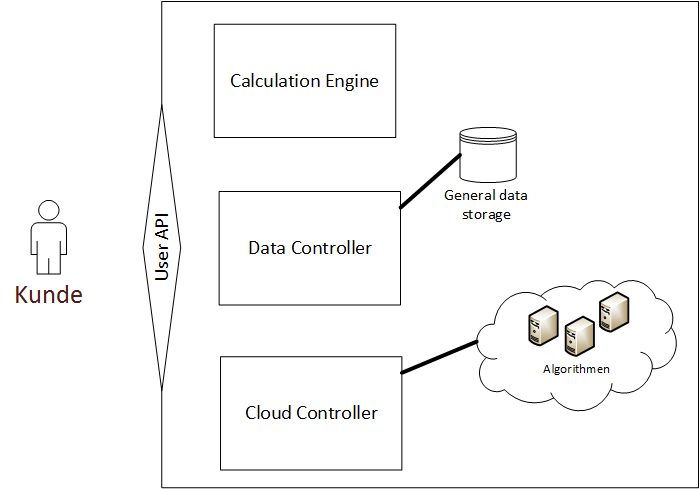
\includegraphics[scale=0.8]{images/visio/ausblick.png}
\caption[Konzept des übergeordneten Projekts]{Konzept des übergeordneten Projekts \selfmade{}}
\label{fig:ausblick}
\end{figure}

\pagenumbering{Roman}

\appendix
\chapter{Anhang}\label{chap.anhang}
%\section{Abnahmeprotokoll}\label{anhang_abnahmeprotokoll}
%\includepdf{images/word/Abnahmeprotokoll.pdf}

\clearpage
 %%%%%%%%%%%%%%%%%%%%%%%%%%%%%%%%%%%%%%%%%%%%%%%%%%%%%%%%%%%%%%%%%
%
% Project     : Bachelorarbeit
% Title       : Machbarkeitsanalyse für eine ressourcenorientierte Schnittstelle zur Verarbeitung grundlegender Probleme der Informatik
% File        : glossar.tex Rev. 01
% Date        : 01.03.2015
% Author      : Raffael Santschi
%
%%%%%%%%%%%%%%%%%%%%%%%%%%%%%%%%%%%%%%%%%%%%%%%%%%%%%%%%%%%%%%%%%

\chapter*{Glossar}\label{glossar}
 \addcontentsline{toc}{chapter}{Glossar}

In diesem Abschnitt werden Abkürzungen und Begriffe kurz erklärt.

\begin{longtable}{>{\raggedright}m{3cm}m{11cm}}

\caption[Glossar]{\label{app_tbl:Abbr}Glossar}\\ 
\toprule
\textbf{Begriff}&\textbf{Bedeutung}\\ \midrule\addlinespace
\endfirsthead
\caption*{\textbf{Tabelle~\ref{app_tbl:Abbr} (Fortsetzung):} Glossar}\\ \toprule
\textbf{Abkürzung}&\textbf{Bedeutung}\\ \midrule\addlinespace
\endhead

\bottomrule\multicolumn{2}{>{\small\raggedleft\arraybackslash}r}{\slshape Fortsetzung auf der nächsten Seite}\\
\endfoot
\bottomrule
\endlastfoot		

	\textbf{API}&
	(siehe \glossarmark{Application Programming Interface})\\ \addlinespace

	\textbf{Application Programming Interface}&
	Application Programming Interace (\glossarmark{API}) ist eine Schnittstelle, über welche anderen Applikationen Leistungen beziehen kann. In diesem Projekt zum Beispiel die Informationen und Funktionen, welche vom Backend zur Verfügung gestellt werden.\\ \addlinespace

	\textbf{Basisfaktor}&
	Basisfaktoren (unterbewusste Anforderungen) muss das System in jedem Fall vollständig erfüllen, sonst stellt sich beim \glossarmark{Stakeholder} massive Unzufriedenheit ein. \cite{req_eng_book}\\ \addlinespace	

	\textbf{Begeisterungsfaktor}&
	Begeisterungsfaktoren (unbewusste Anforderungen) sind Merkmale eines Systems, deren Wert ein \glossarmark{Stakeholder} erst erkennt, wenn er sie selbst ausprobieren kann oder sie vom Requirements Engineer vorgeschlagen werden.\cite{req_eng_book}\\ \addlinespace	

	\textbf{Entity}&
	Entity (auch Entität) ist ein eindeutig zu bestimmendes Daten-Objekt \\ \addlinespace	

	\textbf{Integrated Development Environment}&
	Eine integrierte Entwicklerumgebung (englisch Integrated Development Environment) beinhalten einen Texteditor, Compiler (falls dieser benötigt wird), Debugger, Formatierungsfunktionen und in dem Kontext der App Entwicklung die Möglichkeit der Erstellung von grafischen Benutzeroberflächen.\\ \addlinespace

	\textbf{IDE}&
	(siehe \glossarmark{Integrated Development Environment})\\ \addlinespace

	\textbf{Object-relational mapping}&
	Objektrelationale Abbildung (englisch object-relational mapping, \glossarmark{ORM}) ist eine Technik der Softwareentwicklung, mit der ein in einer objektorientierten Programmiersprache geschriebenes Anwendungsprogramm seine Objekte in einer relationalen Datenbank ablegen kann. Dem Programm erscheint die Datenbank dann als objektorientierte Datenbank, was die Programmierung erleichtert. \cite{wiki_orm}\\ \addlinespace	

	\textbf{Object Query Language}&
	Object Query Language (\glossarmark{OQL}) ist stark an SQL angelehnt, wobei man nicht mit den Spalten der Tabelle, sondern mit den Attributen des Objekts Abfragen erstellt.\\ \addlinespace	

	\textbf{OQL}&
	(siehe \glossarmark{Object Query Language})\\ \addlinespace

	\textbf{ORM}&
	(siehe \glossarmark{Object-relational mapping})\\ \addlinespace

	\textbf{Projektstrukturplan}&
	Ein Synonym für Work Breakdown Structure (WBS): Eine in der Regel an den Liefergegenständen orientierte Anordnung von Projektelementen, die den Gesamtinhalt und -umfang des Projekts strukturiert und definiert.\cite{proj_mgmt_book}\\ \addlinespace	

	\textbf{Refactoring}&
	Eine Veränderung der internen Struktur der Software, welche sie verständlicher und wartbarer macht, jedoch ohne eine Änderung des ursprünglichen Verhaltens zu bewirken.\cite{feathers2004working}\\ \addlinespace		

	\textbf{Representational State Transfer}&
	Representational State Transfer (\glossarmark{REST}) ist ein mögliche Kommunikationsschnittstelle für Webanwendungen und wird vorallem für System-System-Kommunikation verwendet. Nach \glossarmark{REST} liefert eine Web-Seite genau einen Seiteninhalt zurück und das auch bei mehrmaligen Aufrufen.\\ \addlinespace

	\textbf{REST}&
	(siehe \glossarmark{Representational State Transfer})\\ \addlinespace

	\textbf{RESTful}&
	(siehe \glossarmark{Representational State Transfer})\\ \addlinespace

	\textbf{Stakeholder}&
	 Stakeholder sind für den Requirement Engineer wichtige Quellen zur Identifikation möglicher Anforderungen des Systems.\cite{req_eng_book} Ein Stakeholder ist eine Person, die in irgendeiner Weise vom Projekt betroffen ist, jedoch nicht notwendigerweise direkt Einfluss auf den Projektverlauf haben muss.\\ \addlinespace			

\end{longtable}

\todo{AddWebHooks, asynchron, Poll/Push-Prinzip, Eulerischenkreis, Aussagenlogik}


\clearpage
 \bibliography{bibtex/literatur}
 \addcontentsline{toc}{chapter}{Literaturverzeichnis}

\clearpage
 \listoffigures
 \addcontentsline{toc}{chapter}{Abbildungsverzeichnis}

\clearpage
 \listoftables
 \addcontentsline{toc}{chapter}{Tabellenverzeichnis}


\end{document}
